%% The Project Gutenberg EBook of The Consolation of Philosophy, by Boethius
%% 
%% This eBook is for the use of anyone anywhere at no cost and with
%% almost no restrictions whatsoever.  You may copy it, give it away or
%% re-use it under the terms of the Project Gutenberg License included
%% with this eBook or online at www.gutenberg.net
%% 
%% 
%% Title: The Consolation of Philosophy
%% 
%% Author: Boethius
%% 
%% Release Date: December 11, 2004 [EBook #14328]
%% 
%% Language: English
%% 
%% 
%% *** START OF THIS PROJECT GUTENBERG EBOOK THE CONSOLATION OF PHILOSOPHY ***

\documentclass[11pt]{book}

\usepackage{fontspec}
\setmainfont[Numbers=OldStyle]{TeX Gyre Schola}

\usepackage{fancyhdr}
\usepackage{hyperref}
\usepackage[showcrop,showframe,papersize={5.5in,8.5in}]{geometry}

\usepackage[all]{nowidow}

\usepackage[stable]{footmisc}
\usepackage{graphicx}
\usepackage{poetry}

\poemlinenumsfalse
\setlength{\poemindent}{1em}
\addtolength{\poemmaxlinewd}{-2em}
\setlength{\poemhangindent}{2em}
\newenvironment{ipoem}[1]%
  {%
    \centerpoemon{Yet ’gainst their brothers’ lives men point the murderous}
    \setcounter{poemindentevery}{#1}\begin{poem}\footnotesize%
  }%
  {%
    \end{poem}\setcounter{poemindentevery}{0}%
    \centerpoemoff
  }
\newenvironment{vpoem}[1]%
  {%
    \centerpoemon{Down their cheeks unfeigned the tear drops}
    \def\poemvsindentlines{#1}\begin{poem}\footnotesize%
  }%
  {%
    \end{poem}\def\poemvsindentlines{\relax}%
    \centerpoemoff
  }
\centerpoemon{Yet ’gainst their brothers’ lives men point the murderous steel;}

\renewcommand{\chaptername}{Book}
\renewcommand{\thechapter}{\Roman{chapter}}
\renewcommand{\thesection}{\Roman{section}}

\renewcommand{\chaptermark}[1]{\markboth{#1}{}}
\renewcommand{\sectionmark}[1]{\markright{#1}}

% \makeatletter
% \def\@makechapterhead#1{%
%   \vspace*{50\p@}%
%   {\parindent \z@ \raggedright \normalfont
%     \ifnum \c@secnumdepth >\m@ne
%       \if@mainmatter
%         \huge\bfseries \@chapapp\space \thechapter
%         \par\nobreak
%         \vskip 20\p@
%       \fi
%     \fi
%     \interlinepenalty\@M
%     \Huge \bfseries #1\par\nobreak
%     \vskip 40\p@
%   }}
% \makeatother

\newenvironment{abstract}%
  {\noindent \textbf{\scshape Summary} \\ \rightskip1in\itshape\small}%
  {\bigskip}

\newcommand{\simpletitle}{The \\ Consolation of Philosophy \\ of \\ Boethius}

\title{\simpletitle \\[1em] {\small Translated into English Prose and Verse}}

\author{Boethius \\[2em] Translated by H.R. James \\ {\small M.A., CH. CH. Oxford} \\[2em] 1897}

\date{}

\begin{document}

\setlength{\baselineskip}{1.2\baselineskip}

\frontmatter

\thispagestyle{empty}
\hspace{0pt}
\vfill
\begin{center}
  \Large
  \simpletitle
\end{center}
\vfill
\pagebreak

\thispagestyle{empty}
\hspace{0pt}
\vfill

\noindent Produced by Jonathan Ingram, Karina Aleksandrova and the PG Online Distributed Proofreading Team for Project Gutenberg.

\noindent Typeset by Tommy M. McGuire using \LaTeX $2_\epsilon$.

\noindent The font is \TeX\ Gyre Schola.

\pagebreak

\thispagestyle{empty}
\hspace{0pt}
\vfill

% ὄμως δὲ και ἐν τούτοις διαλάμπει τὸ καλὸν,
% ἐπειδὰν φέρῃ τις εὐκόλως πολλὰς καὶ μεγάλας
% ἀτυχίας, μη δι᾿ ἀναλγησίαν, ἀλλὰ γεννάδας
% ὤν καὶ μεγαλόψυχος

\noindent \emph{homôs de kai en toutois dialampei to kalon, epeidan pherê tis eukolôs pollas kai megalas atychias, mê di analgêsian, alla gennadas ôn kai \mbox{megalopsychos.}}

Aristotle's Ethics, I., xi. 12.

\vfill

\pagebreak
\thispagestyle{empty}
\hspace{0pt}
\vfill

\begin{figure}[ht!]
\centering
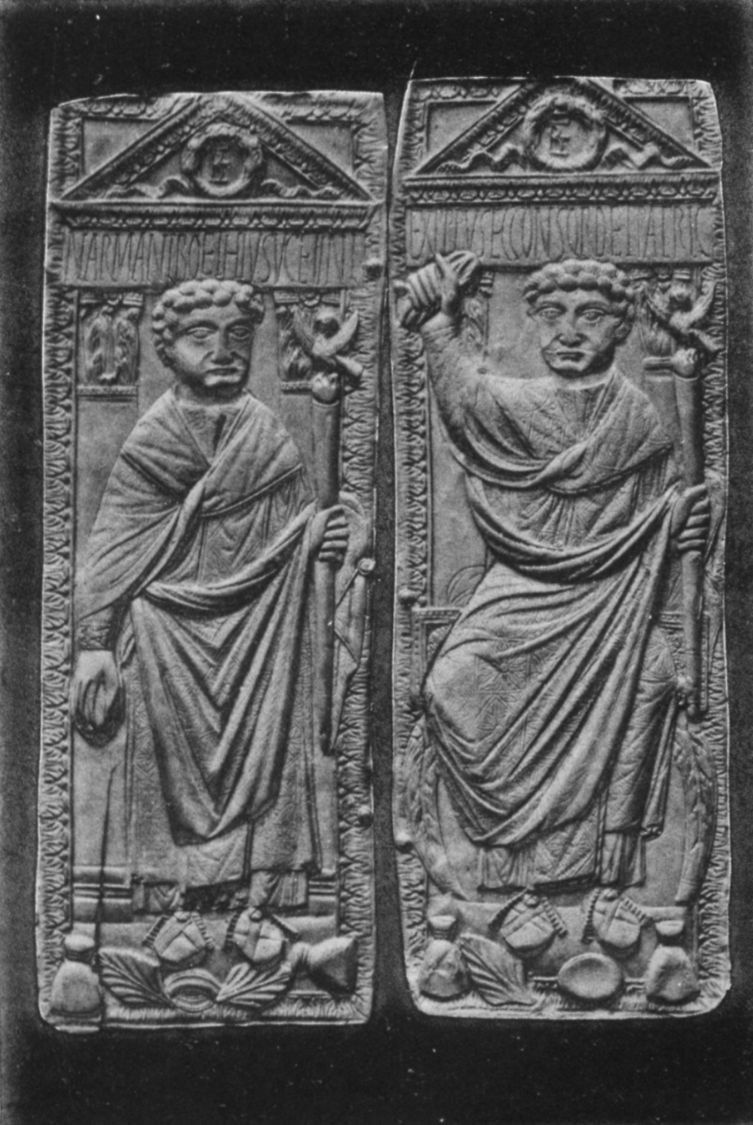
\includegraphics[width=70mm]{image01.jpg}
\caption{Diptych representing Narius Manlius Boethius, father of
Anicius Manlius Severinus Boethius. The inscription in full would run
thus: \textsc{NARivs MANLivs BOETHIVS Vir Clarissimvs ET INLvstris
EXPraefectvs Praetorio Praefectvs VrbiS Et Comes Consvl ORDinarivs ET
PARTICivs} (For description vid. Preface, p.~\pageref{diptych})}
\end{figure}


\vfill

\maketitle

\hspace{0pt}
\vfill

Quantumlibet igitur sæviant mali, sapienti tamen corona non
decidet, non arescet.

Melioribus animum conformaveris, nihil opus est judice præmium      
deferente, tu te ipse excellentioribus addidisti; studium ad pejora     
deflexeris, extra ne quæsieris ultorem, tu te ipse in deteriora        
trusisti.                                                               

\vfill
\pagebreak


\chapter{Preface}

The book called `The Consolation of Philosophy' was \linebreak throughout the
Middle Ages, and down to the beginnings of the modern epoch in the
sixteenth century, the scholar's familiar companion. Few books have
exercised a wider influence in their time. It has been translated into
every European tongue, and into English nearly a dozen times, from King
Alfred's paraphrase to the translations of Lord Preston, Causton,
Ridpath, and Duncan, in the eighteenth century. The belief that what
once pleased so widely must still have some charm is my excuse for
attempting the present translation. The great work of Boethius, with its
alternate prose and verse, skilfully fitted together like dialogue and
chorus in a Greek play, is unique in literature, and has a pathetic
interest from the time and circumstances of its composition. It ought
not to be forgotten. Those who can go to the original will find their
reward. There may be room also for a new translation in English after an
interval of close on a hundred years.

\label{diptych}
Some of the editions contain a reproduction of a bust purporting to
represent Boethius. Lord Preston's translation, for example, has such a
portrait, which it refers to an original in marble at Rome. This I have
been unable to trace, and suspect that it is apocryphal. The Hope
Collection at Oxford contains a completely different portrait in a
print, which gives no authority. I have ventured to use as a
frontispiece a reproduction from a plaster-cast in the Ashmolean Museum,
taken from an ivory diptych preserved in the Bibliotheca Quiriniana at
Brescia, which represents Narius Manlius Boethius, the father of the
philosopher. Portraiture of this period is so rare that it seemed that,
failing a likeness of the author himself, this authentic representation
of his father might have interest, as giving the consular dress and
insignia of the time, and also as illustrating the decadence of
contemporary art. The consul wears a richly-embroidered cloak; his right
hand holds a staff surmounted by the Roman eagle, his left the \emph{mappa
circensis,} or napkin used for starting the races in the circus; at his
feet are palms and bags of money---prizes for the victors in the games.
For permission to use this cast my thanks are due to the authorities of
the Ashmolean Museum, as also to Mr. T.W. Jackson, Curator of the Hope
Collection, who first called my attention to its existence.

I have to thank my brother, Mr. L. James, of Radley College, for much
valuable help and for correcting the proof-sheets of the translation.
The text used is that of Peiper, Leipsic, 1874.

\hspace{0pt}
\vfill

\noindent {\small Take the footnotes with caution; they are probably all wrong. I tried. \emph{TMM}}

\chapter{Proem}

Anicus Manlius Severinus Boethius lived in the last quarter of the fifth
century A.D., and the first quarter of the sixth. He was growing to
manhood, when Theodoric, the famous Ostrogoth, crossed the Alps and made
himself master of Italy. Boethius belonged to an ancient family, which
boasted a connection with the legendary glories of the Republic, and was
still among the foremost in wealth and dignity in the days of Rome's
abasement. His parents dying early, he was brought up by Symmachus, whom
the age agreed to regard as of almost saintly character, and afterwards
became his son-in-law. His varied gifts, aided by an excellent
education, won for him the reputation of the most accomplished man of
his time. He was orator, poet, musician, philosopher. It is his peculiar
distinction to have handed on to the Middle Ages the tradition of Greek
philosophy by his Latin translations of the works of Aristotle. Called
early to a public career, the highest honours of the State came to him
unsought. He was sole Consul in 510 A.D., and was ultimately raised by
Theodoric to the dignity of Magister Officiorum, or head of the whole
civil administration. He was no less happy in his domestic life, in the
virtues of his wife, Rusticiana, and the fair promise of his two sons,
Symmachus and Boethius; happy also in the society of a refined circle of
friends. Noble, wealthy, accomplished, universally esteemed for his
virtues, high in the favour of the Gothic King, he appeared to all men a
signal example of the union of merit and good fortune. His felicity
seemed to culminate in the year 522 A.D., when, by special and
extraordinary favour, his two sons, young as they were for so exalted an
honour, were created joint Consuls and rode to the senate-house
attended by a throng of senators, and the acclamations of the multitude.
Boethius himself, amid the general applause, delivered the public speech
in the King's honour usual on such occasions. Within a year he was a
solitary prisoner at Pavia, stripped of honours, wealth, and friends,
with death hanging over him, and a terror worse than death, in the fear
lest those dearest to him should be involved in the worst results of his
downfall. It is in this situation that the opening of the `Consolation
of Philosophy' brings Boethius before us. He represents himself as
seated in his prison distraught with grief, indignant at the injustice
of his misfortunes, and seeking relief for his melancholy in writing
verses descriptive of his condition. Suddenly there appears to him the
Divine figure of Philosophy, in the guise of a woman of superhuman
dignity and beauty, who by a succession of discourses convinces him of
the vanity of regret for the lost gifts of fortune, raises his mind once
more to the contemplation of the true good, and makes clear to him the
mystery of the world's moral government.

\tableofcontents

%%% INDEX
%%% 
%%% OF
%%% 
%%% VERSE INTERLUDES.
%%% 
%%% 
%%% BOOK I.
%%% THE SORROWS OF BOETHIUS.
%%% 
%%% SONG                                          PAGE
%%%   I. BOETHIUS' COMPLAINT                         3
%%%  II. HIS DESPONDENCY                             9
%%% III. THE MISTS DISPELLED                        12
%%%  IV. NOTHING CAN SUBDUE VIRTUE                  16
%%%   V. BOETHIUS' PRAYER                           27
%%%  VI. ALL THINGS HAVE THEIR NEEDFUL ORDER        33
%%% VII. THE PERTURBATIONS OF PASSION               38
%%% 
%%% 
%%% BOOK II.
%%% THE VANITY OF FORTUNE'S GIFTS.
%%% 
%%%    I. FORTUNE'S MALICE                           47
%%%   II. MAN'S COVETOUSNESS                         51
%%%  III. ALL PASSES                                 55
%%%   IV. THE GOLDEN MEAN                            62
%%%    V. THE FORMER AGE                             70
%%%   VI. NERO'S INFAMY                              76
%%%  VII. GLORY MAY NOT LAST                         82
%%% VIII. LOVE IS LORD OF ALL                        85
%%% 
%%% 
%%% BOOK III.
%%% TRUE HAPPINESS AND FALSE.
%%% 
%%%    I. THE THORNS OF ERROR                        93
%%%   II. THE BENT OF NATURE                         99
%%%  III. THE INSATIABLENESS OK AVARICE             105
%%%   IV. DISGRACE OF HONOURS CONFERRED BY A TYRANT 109
%%%    V. SELF-MASTERY                              113
%%%   VI. TRUE NOBILITY                             116
%%%  VII. PLEASURE'S STING                          118
%%% VIII. HUMAN FOLLY                               121
%%%   IX. INVOCATION                                130
%%%    X. THE TRUE LIGHT                            141
%%%   XI. REMINISCENCE                              150
%%%  XII. ORPHEUS AND EURYDICE                      158
%%% 
%%% 
%%% BOOK IV.
%%% GOOD AND ILL FORTUNE.
%%% 
%%%   I. THE SOUL'S FLIGHT                          166
%%%  II. THE BONDAGE OF PASSION                     177
%%% III. CIRCE'S CUP                                182
%%%  IV. THE UNREASONABLENESS OF HATRED             194
%%%   V. WONDER AND IGNORANCE                       197
%%%  VI. THE UNIVERSAL AIM                          212
%%% VII. THE HERO'S PATH                            219
%%% 
%%% 
%%% BOOK V.
%%% FREE WILL AND GOD'S FOREKNOWLEDGE.
%%% 
%%%   I. CHANCE                                     229
%%%  II. THE TRUE SUN                               233
%%% III. TRUTH'S PARADOXES                          241
%%%  IV. A PSYCHOLOGICAL FALLACY                    250
%%%  V. THE UPWARD LOOK                             255
%%% 

\mainmatter

\chapter{The Sorrows of Boethius}

\begin{abstract}
     Boethius' complaint (Song I.).---CH. I. Philosophy appears to
     Boethius, drives away the Muses of Poetry, and herself laments
     (Song II.) the disordered condition of his mind.---CH. II. \linebreak Boethius
     is speechless with amazement. Philosophy wipes away the tears that
     have clouded his eyesight.---CH. III. Boethius recognises his
     mistress Philosophy. To his wondering inquiries she explains her
     presence, and recalls to his mind the persecutions to which
     Philosophy has oftentimes from of old been subjected by an ignorant
     world. CH. IV. Philosophy bids Boethius declare his griefs. He
     relates the story of his unjust accusation and ruin. He concludes
     with a prayer (Song V.) that the moral disorder in human affairs
     may be set right.---CH. V. Philosophy admits the justice of
     Boethius' self-vindication, but grieves rather for the unhappy
     change in his mind. She will first tranquillize his spirit by
     soothing remedies.---CH. VI. Philosophy tests Boethius' mental
     state by certain questions, and discovers three chief causes of his
     soul's sickness: (1) He has forgotten his own true nature; (2) he
     knows not the end towards which the whole universe tends; (3) he
     knows not the means by which the world is governed.
\end{abstract}

\section{Boethius' complaint}

\begin{ipoem}{2}
    Who wrought my studious numbers \\
      Smoothly once in happier days, \\
    Now perforce in tears and sadness \\
      Learn a mournful strain to raise. \\
    Lo, the Muses, grief-dishevelled, \\
      Guide my pen and voice my woe; \\
    Down their cheeks unfeigned the tear drops \\
      To my sad complainings flow! \\
    These alone in danger's hour \\
      Faithful found, have dared attend \\
    On the footsteps of the exile \\
      To his lonely journey's end. \\
    These that were the pride and pleasure \\
      Of my youth and high estate \\
    Still remain the only solace \\
      Of the old man's mournful fate. \\
    Old? Ah yes; swift, ere I knew it, \\
      By these sorrows on me pressed \\
    Age hath come; lo, Grief hath bid me \\
      Wear the garb that fits her best. \\
    O'er my head untimely sprinkled \\
      These white hairs my woes proclaim, \\
    And the skin hangs loose and shrivelled \\
      On this sorrow-shrunken frame. \\
    Blest is death that intervenes not \\
      In the sweet, sweet years of peace, \\
    But unto the broken-hearted, \\
      When they call him, brings release! \\
    Yet Death passes by the wretched, \\
      Shuts his ear and slumbers deep; \\
    Will not heed the cry of anguish, \\
      Will not close the eyes that weep. \\
    For, while yet inconstant Fortune \\
      Poured her gifts and all was bright, \\
    Death's dark hour had all but whelmed me \\
      In the gloom of endless night. \\
    Now, because misfortune's shadow \\
      Hath o'erclouded that false face, \\
    Cruel Life still halts and lingers, \\
      Though I loathe his weary race. \\
    Friends, why did ye once so lightly \\
      Vaunt me happy among men? \\
    Surely he who so hath fallen \\
      Was not firmly founded then. \\-
\end{ipoem}

While I was thus mutely pondering within myself, and recording       
my sorrowful complainings with my pen, it seemed to me that there       
appeared above my head a \linebreak woman of a countenance exceeding venerable.    
Her eyes were bright as fire, and of a more than human keenness; her    
complexion was lively, her vigour showed no trace of enfeeblement; and  
yet her years were right full, and she plainly seemed not of our age    
and time. Her stature was difficult to judge. At one moment it exceeded 
not the common height, at another her forehead seemed to strike the     
sky; and whenever she raised her head higher, she began to pierce       
within the very heavens, and to baffle the eyes of them that looked     
upon her. Her garments were of an imperishable fabric, wrought with     
the finest threads and of the most delicate workmanship; and these,     
as her own lips afterwards assured me, she had herself woven with her   
own hands. The beauty of this vesture had been somewhat tarnished by    
age and neglect, and wore that dingy look which marble contracts from   
exposure. On the lower-most edge was inwoven the Greek letter $\Pi$,    
on the topmost the letter $\Theta$,\footnote{$\Pi$ stands for the       
Political life, the life of action; $\Theta$ for the Theoretical life,  
the life of thought.} and between the two were to be seen steps, like   
a staircase, from the lower to the upper letter. This robe, moreover,   
had been torn by the hands of violent persons, who had each snatched    
away what he could clutch.\footnote{The Stoic, Epicurean, and other     
philosophical sects, which Boethius regards as heterodox. See also      
below, ch.~\ref{otherPhilosophies}, p.~\pageref{otherPhilosophies}.}    
Her right hand held a note-book; in her left she bore a staff. And      
when she saw the Muses of Poesie standing by my bedside, dictating the  
words of my lamentations, she was moved awhile to wrath, and her eyes   
flashed sternly. `Who,' said she, `has allowed yon play-acting wantons  
to approach this sick man---these who, so far from giving medicine to    
heal his malady, even feed it with sweet poison? These it is who kill   
the rich crop of reason with the barren thorns of passion, who accustom 
men's minds to disease, instead of setting them free. Now, were it some 
common man whom your allurements were seducing, as is usually your way, 
I should be less indignant. On such a one I should not have spent my    
pains for naught. But this is one nurtured in the Eleatic and Academic  
philosophies. Nay, get ye gone, ye sirens, whose sweetness lasteth not; 
leave him for my muses to tend and heal!' At these words of upbraiding, 
the whole band, in deepened sadness, with downcast eyes, and blushes    
that confessed their shame, dolefully left the chamber.                 

But I, because my sight was dimmed with much weeping, and I could not
tell who was this woman of authority so commanding---I was dumfoundered,
and, with my gaze fastened on the earth, continued silently to await
what she might do next. Then she drew near me and sat on the edge of my
couch, and, looking into my face all heavy with grief and fixed in
sadness on the ground, she bewailed in these words the disorder of my
mind:



\section{His despondency}

\begin{vpoem}{24}
    Alas! in what abyss his mind \\
      Is plunged, how wildly tossed! \\
    Still, still towards the outer night \\
      She sinks, her true light lost, \\
    As oft as, lashed tumultuously \\
    By earth-born blasts, care's waves rise high. \\!

    Yet once he ranged the open heavens, \\
      The sun's bright pathway tracked; \\
    Watched how the cold moon waxed and waned; \\
      Nor rested, till there lacked \\
    To his wide ken no star that steers \\
    Amid the maze of circling spheres. \\!

    The causes why the blusterous winds \\
      Vex ocean's tranquil face, \\
    Whose hand doth turn the stable globe, \\
      Or why his even race \\
    From out the ruddy east the sun \\
    Unto the western waves doth run: \\!

    What is it tempers cunningly \\
      The placid hours of spring, \\
    So that it blossoms with the rose \\
      For earth's engarlanding: \\
    Who loads the year's maturer prime \\
    With clustered grapes in autumn time: \\!

    All this he knew---thus ever strove \\
      Deep Nature's lore to guess. \\
    Now, reft of reason's light, he lies, \\
      And bonds his neck oppress; \\
    While by the heavy load constrained, \\
    His eyes to this dull earth are chained. \\-
\end{vpoem}

`But the time,' said she, `calls rather for healing than for
lamentation.' Then, with her eyes bent full upon me, `Art thou that
man,' she cries, `who, erstwhile fed with the milk and reared upon the
nourishment which is mine to give, had grown up to the full vigour of a
manly spirit? And yet I had bestowed such armour on thee as would have
proved an invincible defence, hadst thou not first cast it away. Dost
thou know me? Why art thou silent? Is it shame or amazement that hath
struck thee dumb? Would it were shame; but, as I see, a stupor hath
seized upon thee.' Then, when she saw me not only answering nothing, but
mute and utterly incapable of speech, she gently touched my breast with
her hand, and said: `There is no danger; these are the symptoms of
lethargy, the usual sickness of deluded minds. For awhile he has
forgotten himself; he will easily recover his memory, if only he first
recognises me. And that he may do so, let me now wipe his eyes that are
clouded with a mist of mortal things.' Thereat, with a fold of her robe,
she dried my eyes all swimming with tears.



\section{The mists dispelled}

\begin{ipoem}{2}
    Then the gloom of night was scattered, \\
      Sight returned unto mine eyes. \\
    So, when haply rainy Caurus \\
      Rolls the storm-clouds through the skies, \\
    Hidden is the sun; all heaven \\
      Is obscured in starless night. \\
    But if, in wild onset sweeping, \\
      Boreas frees day's prisoned light, \\
    All suddenly the radiant god outstreams, \\
    And strikes our dazzled eyesight with his beams. \\-
\end{ipoem}


Even so the clouds of my melancholy were broken up. I saw the clear sky,
and regained the power to recognise the face of my physician.
Accordingly, when I had lifted my eyes and fixed my gaze upon her, I
beheld my nurse, Philosophy, whose halls I had frequented from my youth
up.

`Ah! why,' I cried, `mistress of all excellence, hast thou come down
from on high, and entered the solitude of this my exile? Is it that
thou, too, even as I, mayst be persecuted with false accusations?'

`Could I desert thee, child,' said she, `and not lighten the burden  
which thou hast taken upon thee through the hatred of my name, by       
sharing this trouble? Even forgetting that it were not lawful for       
Philosophy to leave companionless the way of the innocent, should I,    
thinkest thou, fear to incur reproach, or shrink from it, as though     
some strange new thing had befallen? Thinkest thou that now, for        
the first time in an evil age, Wisdom hath been assailed by peril?      
Did I not often in days of old, before my servant Plato lived, wage     
stern warfare with the rashness of folly? In his lifetime, too,         
Socrates, his master, won with my aid the victory of an unjust death.   
\label{otherPhilosophies}And when, one after the other, the Epicurean   
herd, the Stoic, and the rest, each of them as far as in them lay,      
went about to seize the heritage he left, and were dragging me off      
protesting and resisting, as their booty, they tore in pieces the       
garment which I had woven with my own hands, and, clutching the torn    
pieces, went off, believing that the whole of me had passed into        
their possession. And some of them, because some traces of my vesture   
were seen upon them, were destroyed through the mistake of the lewd     
multitude, who falsely deemed them to be my disciples. It may be thou   
knowest not of the banishment of Anaxagoras, of the poison draught of   
Socrates, nor of Zeno's torturing, because these things happened in a   
distant country; yet mightest thou have learnt the fate of Arrius, of   
Seneca, of Soranus, whose stories are neither old nor unknown to fame.  
These men were brought to destruction for no other reason than that,    
settled as they were in my principles, their lives were a manifest      
contrast to the ways of the wicked. So there is nothing thou shouldst   
wonder at, if on the seas of this life we are tossed by storm-blasts,   
seeing that we have made it our chiefest aim to refuse compliance       
with evil-doers. And though, maybe, the host of the wicked is many in   
number, yet is it contemptible, since it is under no leadership, but    
is hurried hither and thither at the blind driving of mad error. And    
if at times and seasons they set in array against us, and fall on in    
overwhelming strength, our leader draws off her forces into the citadel 
while they are busy plundering the useless baggage. But we from our     
vantage ground, safe from all this wild work, laugh to see them making  
prize of the most valueless of things, protected by a bulwark which     
aggressive folly may not aspire to reach.'                              



\section{Nothing can subdue virtue}

\begin{ipoem}{0}
    Whoso calm, serene, sedate, \\
    Sets his foot on haughty fate; \\
    Firm and steadfast, come what will, \\
    Keeps his mien unconquered still; \\
    Him the rage of furious seas, \\
    Tossing high wild menaces, \\
    Nor the flames from smoky forges \\
    That Vesuvius disgorges, \\
    Nor the bolt that from the sky \\
    Smites the tower, can terrify. \\
    Why, then, shouldst thou feel affright \\
    At the tyrant's weakling might? \\
    Dread him not, nor fear no harm, \\
    And thou shall his rage disarm; \\
    But who to hope or fear gives way--- \\
    Lost his bosom's rightful sway--- \\
    He hath cast away his shield, \\
    Like a coward fled the field; \\
    He hath forged all unaware \\
    Fetters his own neck must bear! \\-
\end{ipoem}


`Dost thou understand?' she asks. Do my words sink into thy mind? Or art
thou dull ``as the ass to the sound of the lyre''?\footnote{‘Iliad,’ I. 363.} Why dost thou weep? Why
do tears stream from thy eyes?

\begin{quote}
  ```Speak out, hide it not in thy heart''.\footnote{Plato, ‘Republic,’ V. 473, D; Jowett, vol. iii., pp. 170, 171 (3rd edit.).}
\end{quote}

If thou lookest for the physician's help, thou must needs disclose thy
wound.'

Then I, gathering together what strength I could, began: `Is there still
need of telling? Is not the cruelty of fortune against me plain enough?
Doth not the very aspect of this place move thee? Is this the library,
the room which thou hadst chosen as thy constant resort in my home, the
place where we so often sat together and held discourse of all things in
heaven and earth? Was my garb and mien like this when I explored with
thee nature's hid secrets, and thou didst trace for me with thy wand
the courses of the stars, moulding the while my character and the whole
conduct of my life after the pattern of the celestial order? Is this the
recompense of my obedience? Yet thou hast enjoined by Plato's mouth the
maxim, ``that states would be happy, either if philosophers ruled them,
or if it should so befall that their rulers would turn philosophers.''\footnote{Plato, ‘Republic,’ I. 347, C; Jowett, III., p. 25.} By
his mouth likewise thou didst point out this imperative reason why
philosophers should enter public life, to wit, lest, if the reins of
government be left to unprincipled and profligate citizens, trouble and
destruction should come upon the good. Following these precepts, I have
tried to apply in the business of public administration the principles
which I learnt from thee in leisured seclusion. Thou art my witness and
that divinity who hath implanted thee in the hearts of the wise, that I
brought to my duties no aim but zeal for the public good. For this cause
I have become involved in bitter and irreconcilable feuds, and, as
happens inevitably, if a man holds fast to the independence of
conscience, I have had to think nothing of giving offence to the
powerful in the cause of justice. How often have I encountered and
balked Conigastus in his assaults on the fortunes of the weak? How often
have I thwarted Trigguilla, steward of the king's household, even when
his villainous schemes were as good as accomplished? How often have I
risked my position and influence to protect poor wretches from the false
charges innumerable with which they were for ever being harassed by the
greed and license of the barbarians? No one has ever drawn me aside from
justice to oppression. When ruin was overtaking the fortunes of the
provincials through the combined pressure of private rapine and public
taxation, I grieved no less than the sufferers. When at a season of
grievous scarcity a forced sale, disastrous as it was unjustifiable, was
proclaimed, and threatened to overwhelm Campania with starvation, I
embarked on a struggle with the prætorian prefect in the public
interest, I fought the case at the king's judgment-seat, and succeeded
in preventing the enforcement of the sale. I rescued the consular
Paulinus from the gaping jaws of the court bloodhounds, who in their
covetous hopes had already made short work of his wealth. To save
Albinus, who was of the same exalted rank, from the penalties of a
prejudged charge, I exposed myself to the hatred of Cyprian, the
informer.

`Thinkest thou I had laid up for myself store of enmities enough? Well,
with the rest of my countrymen, at any rate, my safety should have been
assured, since my love of justice had left me no hope of security at
court. Yet who was it brought the charges by which I have been struck
down? Why, one of my accusers is Basil, who, after being dismissed from
the king's household, was driven by his debts to lodge an information
against my name. There is Opilio, there is Gaudentius, men who for many
and various offences the king's sentence had condemned to banishment;
and when they declined to obey, and sought to save themselves by taking
sanctuary, the king, as soon as he heard of it, decreed that, if they
did not depart from the city of Ravenna within a prescribed time, they
should be branded on the forehead and expelled. What would exceed the
rigour of this severity? And yet on that same day these very men lodged
an information against me, and the information was admitted. Just
Heaven! had I deserved this by my way of life? Did it make them fit
accusers that my condemnation was a foregone conclusion? Has fortune no
shame---if not at the accusation of the innocent, at least for the
vileness of the accusers? Perhaps thou wonderest what is the sum of the
charges laid against me? I wished, they say, to save the senate. But
how? I am accused of hindering an informer from producing evidence to
prove the senate guilty of treason. Tell me, then, what is thy counsel,
O my mistress. Shall I deny the charge, lest I bring shame on thee? But
I did wish it, and I shall never cease to wish it. Shall I admit it?
Then the work of thwarting the informer will come to an end. Shall I
call the wish for the preservation of that illustrious house a crime?
Of a truth the senate, by its decrees concerning me, has made it such!
But blind folly, though it deceive itself with false names, cannot alter
the true merits of things, and, mindful of the precept of Socrates, I do
not think it right either to keep the truth concealed or allow falsehood
to pass. But this, however it may be, I leave to thy judgment and to the
verdict of the discerning. Moreover, lest the course of events and the
true facts should be hidden from posterity, I have myself committed to
writing an account of the transaction.

`What need to speak of the forged letters by which an attempt is     
made to prove that I hoped for the freedom of Rome? Their falsity       
would have been manifest, if I had been allowed to use the confession   
of the informers themselves, evidence which has in all matters the      
most convincing force. Why, what hope of freedom is left to us? Would   
there were any! I should have answered with the epigram of Canius when  
Caligula declared him to have been cognisant of a conspiracy against    
him. ``If I had known,'' said he, ``thou shouldst never have known.''       
Grief hath not so blunted my perceptions in this matter that I should   
complain because impious wretches contrive their villainies against     
the virtuous, but at their achievement of their hopes I do exceedingly  
marvel. For evil purposes are, perchance, due to the imperfection       
of human nature; that it should be possible for scoundrels to carry     
out their worst schemes against the innocent, while God beholdeth,      
is verily monstrous. For this cause, not without reason, one of thy     
disciples asked, ``If God exists, whence comes evil? Yet whence comes    
good, if He exists not?'' However, it might well be that wretches who    
seek the blood of all honest men and of the whole senate should wish    
to destroy me also, whom they saw to be a bulwark of the senate and     
all honest men. But did I deserve such a fate from the Fathers also?    
Thou rememberest, methinks---since thou didst ever stand by my side      
to direct what I should do or say---thou rememberest, I say, how at      
Verona, when the king, eager for the general destruction, was bent on   
implicating the whole senatorial order in the charge of treason brought 
against Albinus, with what indifference to my own peril I maintained    
the innocence of its members, one and all. Thou knowest that what I     
say is the truth, and that I have never boasted of my good deeds in     
a spirit of self-praise. For whenever a man by proclaiming his good     
deeds receives the recompense of fame, he diminishes in a measure the   
secret reward of a good conscience. What issues have overtaken my       
innocency thou seest. Instead of reaping the rewards of true virtue,    
I undergo the penalties of a guilt falsely laid to my charge---nay,      
more than this; never did an open confession of guilt cause such        
unanimous severity among the assessors, but that some consideration,    
either of the mere frailty of human nature, or of fortune's universal   
instability, availed to soft\-en the verdict of some few. Had I been      
accused of a design to fire the temples, to slaughter the priests with  
impious sword, of plotting the massacre of all honest men, I should yet 
have been produced in court, and only punished on due confession or     
conviction. Now for my too great zeal towards the senate I have been    
condemned to outlawry and death, unheard and undefended, at a distance  
of near five hundred miles away.\footnote{The distance from Rome to     
Pavia, the place of Boethius' imprisonment, is 455 Roman miles.} Oh, my 
judges, well do ye deserve that no one should hereafter be convicted of 
a fault like mine!                                                      

`Yet even my very accusers saw how honourable was the charge they
brought against me, and, in order to overlay it with some shadow of
guilt, they falsely asserted that in the pursuit of my ambition I had
stained my conscience with sacrilegious acts. And yet thy spirit,
indwelling in me, had driven from the chamber of my soul all lust of
earthly success, and with thine eye ever upon me, there could be no
place left for sacrilege. For thou didst daily repeat in my ear and
instil into my mind the Pythagorean maxim, ``Follow after God.'' It was
not likely, then, that I should covet the assistance of the vilest
spirits, when thou wert moulding me to such an excellence as should
conform me to the likeness of God. Again, the innocency of the inner
sanctuary of my home, the company of friends of the highest probity, a
father-in-law revered at once for his pure character and his active
beneficence, shield me from the very suspicion of sacrilege.
Yet---atrocious as it is---they even draw credence for this charge from
\emph{thee}; I am like to be thought implicated in wickedness on this very
account, that I am imbued with \emph{thy} teachings and stablished in \emph{thy}
ways. So it is not enough that my devotion to thee should profit me
nothing, but thou also must be assailed by reason of the odium which I
have incurred. Verily this is the very crown of my misfortunes, that
men's opinions for the most part look not to real merit, but to the
event; and only recognise foresight where Fortune has crowned the issue
with her approval. Whereby it comes to pass that reputation is the first
of all things to abandon the unfortunate. I remember with chagrin how
perverse is popular report, how various and discordant men's judgments.
This only will I say, that the most crushing of misfortune's burdens is,
that as soon as a charge is fastened upon the unhappy, they are believed
to have deserved their sufferings. I, for my part, who have been
banished from all life's blessings, stripped of my honours, stained in
repute, am punished for well-doing.

`And now methinks I see the villainous dens of the wicked surging with
joy and gladness, all the most recklessly unscrupulous threatening a new
crop of lying informations, the good prostrate with terror at my danger,
every ruffian incited by impunity to new daring and to success by the
profits of audacity, the guiltless not only robbed of their peace of
mind, but even of all means of defence. Wherefore I would fain cry out:


\section{Boethius' prayer}

\begin{vpoem}{24568}
    `Builder of yon starry dome, \\
      Thou that whirlest, throned eternal, \\
    Heaven's swift globe, and, as they roam, \\
      Guid'st the stars by laws supernal: \\
        So in full-sphered splendour dight \\
        Cynthia dims the lamps of night, \\
      But unto the orb fraternal \\
        Closer drawn,\footnote{The moon is regarded as farthest from the sun at the full, and, as she wanes, approaching gradually nearer.} doth lose her light. \\!

    `Who at fall of eventide, \\
      Hesper, his cold radiance showeth, \\
    Lucifer his beams doth hide, \\
      Paling as the sun's light groweth, \\
        Brief, while winter's frost holds sway, \\
        By thy will the space of day; \\
      Swift, when summer's fervour gloweth, \\
        Speed the hours of night away. \\!

    `Thou dost rule the changing year: \\
      When rude Boreas oppresses, \\
    Fall the leaves; they reappear, \\
      Wooed by Zephyr's soft caresses. \\
        Fields that Sirius burns deep grown \\
        By Arcturus' watch were sown: \\
      Each the reign of law confesses, \\
        Keeps the place that is his own. \\!

    `Sovereign Ruler, Lord of all! \\
      Can it be that Thou disdainest \\
    Only man? 'Gainst him, poor thrall, \\
      Wanton Fortune plays her vainest. \\
        Guilt's deserved punishment \\
        Falleth on the innocent; \\
      High uplifted, the profanest \\
        On the just their malice vent. \\!

    `Virtue cowers in dark retreats, \\
      Crime's foul stain the righteous beareth, \\
    Perjury and false deceits \\
      Hurt not him the wrong who dareth; \\
        But whene'er the wicked trust \\
        In ill strength to work their lust, \\
      Kings, whom nations' awe declareth \\
        Mighty, grovel in the dust. \\!
 
    `Look, oh look upon this earth, \\
      Thou who on law's sure foundation \\
    Framedst all! Have we no worth, \\
      We poor men, of all creation? \\
        Sore we toss on fortune's tide; \\
        Master, bid the waves subside! \\
      And earth's ways with consummation \\
        Of Thy heaven's order guide!' \\-
\end{vpoem}


When I had poured out my griefs in this long and unbroken strain of
lamentation, she, with calm countenance, and in no wise disturbed at my
complainings, thus spake:

`When I saw thee sorrowful, in tears, I straightway knew thee wretched
and an exile. But how far distant that exile I should not know, had not
thine own speech revealed it. Yet how far indeed from thy country hast
thou, not been banished, but rather hast strayed; or, if thou wilt have
it banishment, hast banished thyself! For no one else could ever
lawfully have had this power over thee. Now, if thou wilt call to mind
from what country thou art sprung, it is not ruled, as once was the
Athenian polity, by the sovereignty of the multitude, but ``one is its
Ruler, one its King,''\footnote{‘Iliad,’ II., 204, 205.} who takes delight in the number of His citizens,
not in their banishment; to submit to whose governance and to obey
whose ordinances is perfect freedom. Art thou ignorant of that most
ancient law of this thy country, whereby it is decreed that no one
whatsoever, who hath chosen to fix there his dwelling, may be sent into
exile? For truly there is no fear that one who is encompassed by its
ramparts and defences should deserve to be exiled. But he who has ceased
to wish to dwell therein, he likewise ceases to deserve to do so. And so
it is not so much the aspect of this place which moves me, as thy
aspect; not so much the library walls set off with glass and ivory which
I miss, as the chamber of thy mind, wherein I once placed, not books,
but that which gives books their value, the doctrines which my books
contain. Now, what thou hast said of thy services to the commonweal is
true, only too little compared with the greatness of thy deservings. The
things laid to thy charge whereof thou hast spoken, whether such as
redound to thy credit, or mere false accusations, are publicly known. As
for the crimes and deceits of the informers, thou hast rightly deemed
it fitting to pass them over lightly, because the popular voice hath
better and more fully pronounced upon them. Thou hast bitterly
complained of the injustice of the senate. Thou hast grieved over my
calumniation, and likewise hast lamented the damage to my good name.
Finally, thine indignation blazed forth against fortune; thou hast
complained of the unfairness with which thy merits have been
recompensed. Last of all thy frantic muse framed a prayer that the peace
which reigns in heaven might rule earth also. But since a throng of
tumultuous passions hath assailed thy soul, since thou art distraught
with anger, pain, and grief, strong remedies are not proper for thee in
this thy pres\-ent mood. And so for a time I will use milder methods, that
the tumours which have grown hard through the influx of disturbing
passion may be softened by gentle treatment, till they can bear the
force of sharper remedies.'


\section{All things have their needful order}

\begin{vpoem}{24}
    He who to th' unwilling furrows \\
      Gives the generous grain, \\
    When the Crab with baleful fervours \\
      Scorches all the plain; \\
    He shall find his garner bare, \\
    Acorns for his scanty fare. \\!

    Go not forth to cull sweet violets \\
      From the purpled steep, \\
    While the furious blasts of winter \\
      Through the valleys sweep; \\
    Nor the grape o'erhasty bring \\
    To the press in days of spring. \\!

    For to each thing God hath given \\
      Its appointed time; \\
    No perplexing change permits He \\
      In His plan sublime. \\
    So who quits the order due \\
    Shall a luckless issue rue. \\-
\end{vpoem}


`First, then, wilt thou suffer me by a few questions to make some
attempt to test the state of thy mind, that I may learn in what way to
set about thy cure?'

`Ask what thou wilt,' said I, `for I will answer whatever questions thou
choosest to put.'

Then said she: `This world of ours---thinkest thou it is governed
haphazard and fortuitously, or believest thou that there is in it any
rational guidance?'

`Nay,' said I, `in no wise may I deem that such fixed motions can be
determined by random hazard, but I know that God, the Creator, presideth
over His work, nor will the day ever come that shall drive me from
holding fast the truth of this belief.'

`Yes,' said she; `thou didst even but now affirm it in song, lamenting
that men alone had no portion in the divine care. As to the rest, thou
wert unshaken in the belief that they were ruled by reason. Yet I
marvel exceedingly how, in spite of thy firm hold on this opinion, thou
art fallen into sickness. But let us probe more deeply: something or
other is missing, I think. Now, tell me, since thou doubtest not that
God governs the world, dost thou perceive by what means He rules it?'

`I scarcely understand what thou meanest,' I said, `much less can I
answer thy question.'

`Did I not say truly that something is missing, where\-by, as through a
breach in the ramparts, disease hath crept in to disturb thy mind? But,
tell me, dost thou remember the universal end towards which the aim of
all nature is directed?'

`I once heard,' said I, `but sorrow hath dulled my recollection.'

`And yet thou knowest whence all things have proceeded.'

`Yes, that I know,' said I, `and have answered that it is from God.'

`Yet how is it possible that thou knowest not what is the end of
existence, when thou dost understand its source and origin? However,
these disturbances of mind have force to shake a man's position, but
cannot pluck him up and root him altogether out of himself. But answer
this also, I pray thee: rememberest thou that thou art a man?'

`How should I not?' said I.

`Then, canst thou say what man is?'

`Is this thy question: Whether I know myself for a being endowed with
reason and subject to death? Surely I do acknowledge myself such.'

Then she: `Dost know nothing else that thou art?'

`Nothing.'

`Now,' said she, `I know another cause of thy disease, one, too, of
grave moment. Thou hast ceased to know thy own nature. So, then, I have
made full discovery both of the causes of thy sickness and the means of
restoring thy health. It is because forgetfulness of thyself hath
bewildered thy mind that thou hast bewailed thee as an exile, as one
stripped of the blessings that were his; it is because thou knowest not
the end of existence that thou deemest abominable and wicked men to be
happy and powerful; while, because thou hast forgotten by what means the
earth is governed, thou deemest that fortune's changes ebb and flow
without the restraint of a guiding hand. These are serious enough to
cause not sickness only, but even death; but, thanks be to the Author of
our health, the light of nature hath not yet left thee utterly. In thy
true judgment concerning the world's government, in that thou believest
it subject, not to the random drift of chance, but to divine reason, we
have the divine spark from which thy recovery may be hoped. Have, then,
no fear; from these weak embers the vital heat shall once more be
kindled within thee. But seeing that it is not yet time for strong
remedies, and that the mind is manifestly so constituted that when it
casts off true opinions it straightway puts on false, wherefrom arises a
cloud of confusion that disturbs its true vision, I will now try and
disperse these mists by mild and soothing application, that so the
darkness of misleading passion may be scattered, and thou mayst come to
discern the splendour of the true light.'


\section{The perturbations of passion}

\begin{vpoem}{2356}
    Stars shed no light \\
      Through the black night, \\
        When the clouds hide; \\
    And the lashed wave, \\
      If the winds rave \\
        O'er ocean's tide,--- \\!

    Though once serene \\
      As day's fair sheen,--- \\
        Soon fouled and spoiled \\
    By the storm's spite, \\
      Shows to the sight \\
        Turbid and soiled. \\!

    Oft the fair rill, \\
      Down the steep hill \\
        Seaward that strays, \\
    Some tumbled block \\
      Of fallen rock \\
        Hinders and stays. \\!

    Then art thou fain \\
      Clear and most plain \\
        Truth to discern, \\
    In the right way \\
      Firmly to stay, \\
        Nor from it turn? \\!

    Joy, hope and fear \\
      Suffer not near, \\
        Drive grief away: \\
    Shackled and blind \\
      And lost is the mind \\
        Where these have sway. \\-
\end{vpoem}

\chapter{The Vanity of Fortune's Gifts}

\begin{abstract}
     CH. I. Philosophy reproves Boethius for the foolishness of his
     complaints against Fortune. Her very nature is caprice.---CH. II.
     Philosophy in Fortune's name replies to Boethius' reproaches, and
     proves that the gifts of Fortune are hers to give and to take
     away.---CH. III. Boethius falls back upon his pres\-ent sense of
     misery. Philosophy reminds him of the brilliancy of his former
     fortunes.---CH. IV. Boethius objects that the memory of past
     happiness is the bitterest portion of the lot of the unhappy.
     Philosophy shows that much is still left for which he may be
     thankful. None enjoy perfect satisfaction with their lot. But
     happiness depends not on anything which Fortune can give. It is to
     be sought within.---CH. V. All the gifts of Fortune are external;
     they can never truly be our own. Man cannot find his good in
     worldly possessions. Riches bring anxiety and trouble.---CH. VI.
     High place without virtue is an evil, not a good. Power is an empty
     name.---CH. VII. Fame is a thing of little account when compared
     with the immensity of the Universe and the endlessness of
     Time.---CH. VIII. One service only can Fortune do, when she reveals
     her own nature and distinguishes true friends from false.
\end{abstract}





Thereafter for awhile she remained silent; and when she had restored my
flagging attention by a moderate pause in her discourse, she thus began:
`If I have thoroughly ascertained the character and causes of thy
sickness, thou art pining with regretful longing for thy former fortune.
It is the change, as thou deemest, of this fortune that hath so wrought
upon thy mind. Well do I understand that Siren's manifold wiles, the
fatal charm of the friendship she pretends for her victims, so long as
she is scheming to entrap them---how she unexpectedly abandons them and
leaves them overwhelmed with insupportable grief. Bethink thee of her
nature, character, and deserts, and thou wilt soon acknowledge that in
her thou hast neither possessed, nor hast thou lost, aught of any worth.
Methinks I need not spend much pains in bringing this to thy mind,
since, even when she was still with thee, even while she was caressing
thee, thou usedst to assail her in manly terms, to rebuke her, with
maxims drawn from my holy treasure-house. But all sudden changes of
circumstances bring inevitably a certain commotion of spirit. Thus it
hath come to pass that thou also for awhile hast been parted from thy
mind's tranquillity. But it is time for thee to take and drain a
draught, soft and pleasant to the taste, which, as it penetrates within,
may prepare the way for stronger potions. Wherefore I call to my aid the
sweet persuasiveness of Rhetoric, who then only walketh in the right way
when she forsakes not my instructions, and Music, my handmaid, I bid to
join with her singing, now in lighter, now in graver strain.

`What is it, then, poor mortal, that hath cast thee into lamentation and
mourning? Some strange, un\-wont\-ed sight, methinks, have thine eyes seen.
Thou deemest Fortune to have changed towards thee; thou mistakest. Such
ever were her ways, ever such her nature. Rather in her very mutability
hath she preserved towards thee her true constancy. Such was she when
she loaded thee with caresses, when she deluded thee with the
allurements of a false happiness. Thou hast found out how changeful is
the face of the blind goddess. She who still veils herself from others
hath fully discovered to thee her whole character. If thou likest her,
take her as she is, and do not complain. If thou abhorrest her perfidy,
turn from her in disdain, renounce her, for baneful are her delusions.
The very thing which is now the cause of thy great grief ought to have
brought thee tranquillity. Thou hast been forsaken by one of whom no one
can be sure that she will not forsake him. Or dost thou indeed set value
on a happiness that is certain to depart? Again I ask, Is Fortune's
presence dear to thee if she cannot be trusted to stay, and though she
will bring sorrow when she is gone? Why, if she cannot be kept at
pleasure, and if her flight overwhelms with calamity, what is this
fleeting visitant but a token of coming trouble? Truly it is not enough
to look only at what lies before the eyes; wisdom gauges the issues of
things, and this same mutability, with its two aspects, makes the
threats of Fortune void of terror, and her caresses little to be
desired. Finally, thou oughtest to bear with whatever takes place within
the boundaries of Fortune's demesne, when thou hast placed thy head
beneath her yoke. But if thou wishest to impose a law of staying and
departing on her whom thou hast of thine own accord chosen for thy
mistress, art thou not acting wrongfully, art thou not embittering by
impatience a lot which thou canst not alter? Didst thou commit thy sails
to the winds, thou wouldst voyage not whither thy intention was to go,
but whither the winds drave thee; didst thou entrust thy seed to the
fields, thou wouldst set off the fruitful years against the barren. Thou
hast resigned thyself to the sway of Fortune; thou must submit to thy
mistress's caprices. What! art thou verily striving to stay the swing
of the revolving wheel? Oh, stupidest of mortals, if it takes to
standing still, it ceases to be the wheel of Fortune.'


\section{Fortune's malice}


\begin{ipoem}{0}
    Mad Fortune sweeps along in wanton pride, \\
    Uncertain as Euripus' surging tide; \\
    Now tramples mighty kings beneath her feet; \\
    Now sets the conquered in the victor's seat. \\
    She heedeth not the wail of hapless woe, \\
    But mocks the griefs that from her mischief flow. \\
    Such is her sport; so proveth she her power; \\
    And great the marvel, when in one brief hour \\
    She shows her darling lifted high in bliss, \\
    Then headlong plunged in misery's abyss. \\-
\end{ipoem}



`Now I would fain also reason with thee a little in Fortune's own words.
Do thou observe whether her contentions be just. ``Man,'' she might say,
``why dost thou pursue me with thy daily complainings? What wrong have I
done thee? What goods of thine have I taken from thee? Choose an thou
wilt a judge, and let us dispute before him concerning the rightful
ownership of wealth and rank. If thou succeedest in showing that any one
of these things is the true property of mortal man, I freely grant those
things to be thine which thou claimest. When nature brought thee forth
out of thy mother's womb, I took thee, naked and destitute as thou wast,
I cherished thee with my substance, and, in the partiality of my favour
for thee, I brought thee up somewhat too indulgently, and this it is
which now makes thee rebellious against me. I surrounded thee with a
royal abundance of all those things that are in my power. Now it is my
pleasure to draw back my hand. Thou hast reason to thank me for the use
of what was not thine own; thou hast no right to complain, as if thou
hadst lost what was wholly thine. Why, then, dost bemoan thyself? I have
done thee no violence. Wealth, honour, and all such things are placed
under my control. My handmaidens know their mistress; with me they come,
and at my going they depart. I might boldly affirm that if those things
the loss of which thou lamentest had been thine, thou couldst never have
lost them. Am I alone to be forbidden to do what I will with my own?
Unrebuked, the skies now reveal the brightness of day, now shroud the
daylight in the darkness of night; the year may now engarland the face
of the earth with flowers and fruits, now disfigure it with storms and
cold. The sea is permitted to invite with smooth and tranquil surface
to-day, to-morrow to roughen with wave and storm. Shall man's insatiate
greed bind \emph{me} to a constancy foreign to my character? This is my art,
this the game I never cease to play. I turn the wheel that spins. I
delight to see the high come down and the low ascend. Mount up, if thou
wilt, but only on condition that thou wilt not think it a hardship to
come down when the rules of my game require it. Wert thou ignorant of my
character? Didst not know how Croesus, King of the Lydians, erstwhile
the dreaded rival of Cyrus, was afterwards pitiably consigned to the
flame of the pyre, and only saved by a shower sent from heaven? Has it
'scaped thee how Paullus paid a meed of pious tears to the misfortunes
of King Perseus, his prisoner? What else do tragedies make such woeful
outcry over save the overthrow of kingdoms by the indiscriminate strokes
of Fortune? Didst thou not learn in thy childhood how there stand at the
threshold of Zeus ``two jars,''\footnote{‘Iliad.’ XXIV. 527, 528.}
``the one full of blessings, the other of
calamities''? How if thou hast drawn over-liberally from the good jar?
What if not even now have I departed wholly from thee? What if this very
mutability of mine is a just ground for hoping better things? But listen
now, and cease to let thy heart consume away with fretfulness, nor
expect to live on thine own terms in a realm that is common to all.'



%SONG II.

\section{Man's covetousness}

\begin{ipoem}{2}
    What though Plenty pour her gifts \\
      With a lavish hand, \\
    Numberless as are the stars, \\
      Countless as the sand, \\
    Will the race of man, content, \\
    Cease to murmur and lament? \\!
 
    Nay, though God, all-bounteous, give \\
      Gold at man's desire--- \\
    Honours, rank, and fame---content \\
      Not a whit is nigher; \\
    But an all-devouring greed \\
    Yawns with ever-widening need. \\!

    Then what bounds can e'er restrain \\
      This wild lust of having, \\
    When with each new bounty fed \\
      Grows the frantic craving? \\
    He is never rich whose fear \\
    Sees grim Want forever near. \\-
\end{ipoem}


`If Fortune should plead thus against thee, assuredly thou wouldst not
have one word to offer in reply; or, if thou canst find any
justification of thy complainings, thou must show what it is. I will
give thee space to speak.'

Then said I: `Verily, thy pleas are plausible---yea, \linebreak steeped in the
honeyed sweetness of music and rhetoric. But their charm lasts only
while they are sounding in the ear; the sense of his misfortunes lies
deeper in the heart of the wretched. So, when the sound ceases to
vibrate upon the air, the heart's indwelling sorrow is felt with renewed
bitterness.'

Then said she: `It is indeed as thou sayest, for we have not yet come to
the curing of thy sickness; as yet these are but lenitives conducing to
the treatment of a malady hitherto obstinate. The remedies which go deep
I will apply in due season. Nevertheless, to deprecate thy
determination to be thought wretched, I ask thee, Hast thou forgotten
the extent and bounds of thy felicity? I say nothing of how, when
orphaned and desolate, thou wast taken into the care of illustrious men;
how thou wast chosen for alliance with the highest in the state---and
even before thou wert bound to their house by marriage, wert already
dear to their love---which is the most precious of all ties. Did not all
pronounce thee most happy in the virtues of thy wife, the splendid
honours of her father, and the blessing of male issue? I pass over---for
I care not to speak of blessings in which others also have shared---the
distinctions often denied to age which thou enjoyedst in thy youth. I
choose rather to come to the unparalleled culmination of thy good
fortune. If the fruition of any earthly success has weight in the scale
of happiness, can the memory of that splendour be swept away by any
rising flood of troubles? That day when thou didst see thy two sons ride
forth from home joint consuls, followed by a train of senators, and
welcomed by the good-will of the people; when these two sat in curule
chairs in the Senate-house, and thou by thy panegyric on the king didst
earn the fame of eloquence and ability; when in the Circus, seated
between the two consuls, thou didst glut the multitude thronging around
with the triumphal largesses for which they looked---methinks thou didst
cozen Fortune while she caressed thee, and made thee her darling. Thou
didst bear off a boon which she had never before granted to any private
person. Art thou, then, minded to cast up a reckoning with Fortune? Now
for the first time she has turned a jealous glance upon thee. If thou
compare the extent and bounds of thy blessings and misfortunes, thou
canst not deny that thou art still fortunate. Or if thou esteem not
thyself favoured by Fortune in that thy then seeming prosperity hath
departed, deem not thyself wretched, since what thou now believest to be
calamitous passeth also. What! art thou but now come suddenly and a
stranger to the scene of this life? Thinkest thou there is any stability
in human affairs, when man himself vanishes away in the swift course of
time? It is true that there is little trust that the gifts of chance
will abide; yet the last day of life is in a manner the death of all
remaining Fortune. What difference, then, thinkest thou, is there,
whether thou leavest her by dying, or she leave thee by fleeing away?'



%SONG III.

\section{All passes}

\begin{ipoem}{0}
    When, in rosy chariot drawn, \\
    Phoebus 'gins to light the dawn, \\
    By his flaming beams assailed, \\
    Every glimmering star is paled. \\
    When the grove, by Zephyrs fed, \\
    With rose-blossom blushes red;--- \\
    Doth rude Auster breathe thereon, \\
    Bare it stands, its glory gone. \\
    Smooth and tranquil lies the deep \\
    While the winds are hushed in sleep. \\
    Soon, when angry tempests lash, \\
    Wild and high the billows dash. \\
    Thus if Nature's changing face \\
    Holds not still a moment's space, \\
    Fleeting deem man's fortunes; deem \\
    Bliss as transient as a dream. \\
    One law only standeth fast: \\
    Things created may not last. \\-
\end{ipoem}

Then said I: `True are thine admonishings, thou nurse of all excellence;
nor can I deny the wonder of my fortune's swift career. Yet it is this
which chafes me the more cruelly in the recalling. For truly in adverse
fortune the worst sting of misery is to \emph{have been} happy.'

`Well,' said she, `if thou art paying the penalty of a mistaken belief,
thou canst not rightly impute the fault to circumstances. If it is the
felicity which Fortune gives that moves thee---mere name though it
be---come reckon up with me how rich thou art in the number and
weightiness of thy blessings. Then if, by the blessing of Providence,
thou hast still preserved unto thee safe and inviolate that which,
howsoever thou mightest reckon thy fortune, thou wouldst have thought
thy most precious possession, what right hast thou to talk of
ill-fortune whilst keeping all Fortune's better gifts? Yet Symmachus,
thy wife's father---a man whose splendid character does honour to the
human race---is safe and unharmed; and while he bewails thy wrongs, this
rare nature, in whom wisdom and virtue are so nobly blended, is himself
out of danger---a boon thou wouldst have been quick to purchase at the
price of life itself. Thy wife yet lives, with her gentle disposition,
her peerless modesty and virtue---this the epitome of all her graces,
that she is the true daughter of her sire---she lives, I say, and for thy
sake only preserves the breath of life, though she loathes it, and pines
away in grief and tears for thy absence, where\-in, if in naught else, I
would allow some marring of thy felicity. What shall I say of thy sons
and their consular dignity---how in them, so far as may be in youths of
their age, the example of their father's and grandfather's character
shines out? Since, then, the chief care of mortal man is to preserve his
life, how happy art thou, couldst thou but recognise thy blessings, who
possessest even now what no one doubts to be dearer than life!
Wherefore, now dry thy tears. Fortune's hate hath not involved all thy
dear ones; the stress of the storm that has assailed thee is not beyond
measure intolerable, since there are anchors still holding firm which
suffer thee not to lack either consolation in the present or hope for
the future.'

`I pray that they still may hold. For while they still remain, however
things may go, I shall ride out the storm. Yet thou seest how much is
shorn of the splendour of my fortunes.'

`We are gaining a little ground,' said she, `if there is something in
thy lot wherewith thou art not yet altogether discontented. But I cannot
stomach thy daintiness when thou complainest with such violence of grief
and anxiety because thy happiness falls short of completeness. Why, who
enjoys such settled felicity as not to have some quarrel with the
circumstances of his lot? A troublous matter are the conditions of human
bliss; either they are never realized in full, or never stay
permanently. One has abundant riches, but is shamed by his ignoble
birth. Another is conspicuous for his nobility, but through the
embarrassments of poverty would prefer to be obscure. A third, richly
endowed with both, laments the loneliness of an unwedded life. Another,
though happily married, is doomed to childlessness, and nurses his
wealth for a stranger to inherit. Yet another, blest with children,
mournfully bewails the misdeeds of son or daughter. Wherefore, it is not
easy for anyone to be at perfect peace with the circumstances of his
lot. There lurks in each several portion something which they who
experience it not know nothing of, but which makes the sufferer wince.
Besides, the more favoured a man is by Fortune, the more fastidiously
sensitive is he; and, unless all things answer to his whim, he is
overwhelmed by the most trifling misfortunes, because utterly unschooled
in adversity. So petty are the trifles which rob the most fortunate of
perfect happiness! How many are there, dost thou imagine, who would
think themselves nigh heaven, if but a small portion from the wreck of
thy fortune should fall to them? This very place which thou callest
exile is to them that dwell therein their native land. So true is it
that nothing is wretched, but thinking makes it so, and conversely every
lot is happy if borne with equanimity. Who is so blest by Fortune as not
to wish to change his state, if once he gives rein to a rebellious
spirit? With how many bitternesses is the sweetness of human felicity
blent! And even if that sweetness seem to him to bring delight in the
enjoying, yet he cannot keep it from departing when it will. How
manifestly wretched, then, is the bliss of earthly fortune, which lasts
not for ever with those whose temper is equable, and can give no perfect
satisfaction to the anxious-minded!

`Why, then, ye children of mortality, seek ye from without that
happiness whose seat is only within us? Error and ignorance bewilder
you. I will show thee, in brief, the hinge on which perfect happiness
turns. Is there anything more precious to thee than thyself? Nothing,
thou wilt say. If, then, thou art master of thyself, thou wilt possess
that which thou wilt never be willing to lose, and which Fortune cannot
take from thee. And that thou mayst see that happiness cannot possibly
consist in these things which are the sport of chance, reflect that, if
happiness is the highest good of a creature living in accordance with
reason, and if a thing which can in any wise be reft away is not the
highest good, since that which cannot be taken away is better than it,
it is plain that Fortune cannot aspire to bestow happiness by reason of
its instability. And, besides, a man borne along by this transitory
felicity must either know or not know its unstability. If he knows not,
how poor is a happiness which depends on the blindness of ignorance! If
he knows it, he needs must fear to lose a happiness whose loss he
believes to be possible. Wherefore, a never-ceasing fear suffers him not
to be happy. Or does he count the possibility of this loss a trifling
matter? Insignificant, then, must be the good whose loss can be borne so
equably. And, further, I know thee to be one settled in the belief that
the souls of men certainly die not with them, and convinced thereof by
numerous proofs; it is clear also that the felicity which Fortune
bestows is brought to an end with the death of the body: therefore, it
cannot be doubted but that, if happiness is conferred in this way, the
whole human race sinks into misery when death brings the close of all.
But if we know that many have sought the joy of happiness not through
death only, but also through pain and suffering, how can life make men
happy by its presence when it makes them not wretched by its loss?'



%SONG IV.

\section{The golden mean}

\begin{ipoem}{0}
    Who founded firm and sure \\
    Would ever live secure, \\
    In spite of storm and blast \\
    Immovable and fast; \\
    Whoso would fain deride \\
    The ocean's threatening tide;--- \\
    His dwelling should not seek \\
    On sands or mountain-peak. \\
    Upon the mountain's height \\
    The storm-winds wreak their spite: \\
    The shifting sands disdain \\
    Their burden to sustain. \\
    Do thou these perils flee, \\
    Fair though the prospect be, \\
    And fix thy resting-place \\
    On some low rock's sure base. \\
    Then, though the tempests roar, \\
    Seas thunder on the shore, \\
    Thou in thy stronghold blest \\
    And undisturbed shalt rest; \\
    Live all thy days serene, \\
    And mock the heavens' spleen. \\-
\end{ipoem}


`But since my reasonings begin to work a soothing effect within thy
mind, methinks I may resort to remedies somewhat stronger. Come,
suppose, now, the gifts of Fortune were not fleeting and transitory,
what is there in them capable of ever becoming truly thine, or which
does not lose value when looked at steadily and fairly weighed in the
balance? Are riches, I pray thee, precious either through thy nature or
in their own? What are they but mere gold and heaps of money? Yet these
fine things show their quality better in the spending than in the
hoarding; for I suppose 'tis plain that greed Alva's makes men hateful,
while liberality brings fame. But that which is transferred to another
cannot remain in one's own possession; and if that be so, then money is
only precious when it is given away, and, by being transferred to
others, ceases to be one's own. Again, if all the money in the world
were heaped up in one man's possession, all others would be made poor.
Sound fills the ears of many at the same time without being broken into
parts, but your riches cannot pass to many without being lessened in the
process. And when this happens, they must needs impoverish those whom
they leave. How poor and cramped a thing, then, is riches, which more
than one cannot possess as an unbroken whole, which falls not to any one
man's lot without the impoverishment of everyone else! Or is it the
glitter of gems that allures the eye? Yet, how rarely excellent soever
may be their splendour, remember the flashing light is in the jewels,
not in the man. Indeed, I greatly marvel at men's admiration of them;
for what can rightly seem beautiful to a being endowed with life and
reason, if it lack the movement and structure of life? And although such
things do in the end take on them more beauty from their Maker's care
and their own brilliancy, still they in no wise merit your admiration
since their excellence is set at a lower grade than your own.

`Does the beauty of the fields delight you? Surely, yes; it is a
beautiful part of a right beautiful whole. Fitly indeed do we at times
enjoy the serene calm of the sea, admire the sky, the stars, the moon,
the sun. Yet is any of these thy concern? Dost thou venture to boast
thyself of the beauty of any one of them? Art \emph{thou} decked with
spring's flowers? is it \emph{thy} fertility that swelleth in the fruits of
autumn? Why art thou moved with empty transports? why embracest thou an
alien excellence as thine own? Never will fortune make thine that which
the nature of things has excluded from thy ownership. Doubtless the
fruits of the earth are given for the sustenance of living creatures.
But if thou art content to supply thy wants so far as suffices nature,
there is no need to resort to fortune's bounty. Nature is content with
few things, and with a very little of these. If thou art minded to force
superfluities upon her when she is satisfied, that which thou addest
will prove either unpleasant or harmful. But, now, thou thinkest it
fine to shine in raiment of divers colours; yet---if, indeed, there is
any pleasure in the sight of such things---it is the texture or the
artist's skill which I shall admire.

`Or perhaps it is a long train of servants that makes thee happy? Why,
if they behave viciously, they are a ruinous burden to thy house, and
exceeding dangerous to their own master; while if they are honest, how
canst thou count other men's virtue in the sum of thy possessions? From
all which 'tis plainly proved that not one of these things which thou
reckonest in the number of thy possessions is really thine. And if there
is in them no beauty to be desired, why shouldst thou either grieve for
their loss or find joy in their continued possession? While if they are
beautiful in their own nature, what is that to thee? They would have
been not less pleasing in themselves, though never included among thy
possessions. For they derive not their preciousness from being counted
in thy riches, but rather thou hast chosen to count them in thy riches
because they seemed to thee precious.

`Then, what seek ye by all this noisy outcry about fortune? To chase
away poverty, I ween, by means of abundance. And yet ye find the result
just contrary. Why, this varied array of precious furniture needs more
accessories for its protection; it is a true saying that they want most
who possess most, and, conversely, they want very little who measure
their abundance by nature's requirements, not by the superfluity of vain
display. Have ye no good of your own implanted within you, that ye seek
your good in things external and separate? Is the nature of things so
reversed that a creature divine by right of reason can in no other way
be splendid in his own eyes save by the possession of lifeless chattels?
Yet, while other things are content with their own, ye who in your
intellect are God-like seek from the lowest of things adornment for a
nature of supreme excellence, and perceive not how great a wrong ye do
your Maker. His will was that mankind should excel all things on earth.
Ye thrust down your worth beneath the lowest of things. For if that in
which each thing finds its good is plainly more precious than that whose
good it is, by your own estimation ye put yourselves below the vilest of
things, when ye deem these vile things to be your good: nor does this
fall out undeservedly. Indeed, man is so constituted that he then only
excels other things when he knows himself; but he is brought lower than
the beasts if he lose this self-knowledge. For that other creatures
should be ignorant of themselves is natural; in man it shows as a
defect. How extravagant, then, is this error of yours, in thinking that
anything can be embellished by adornments not its own. It cannot be. For
if such accessories add any lustre, it is the accessories that get the
praise, while that which they veil and cover remains in its pristine
ugliness. And again I say, That is no \emph{good}, which injures its
possessor. Is this untrue? No, quite true, thou sayest. And yet riches
have often hurt those that possessed them, since the worst of men, who
are all the more covetous by reason of their wickedness, think none but
themselves worthy to possess all the gold and gems the world contains.
So thou, who now dreadest pike and sword, mightest have trolled a carol
``in the robber's face,'' hadst thou entered the road of life with empty
pockets. Oh, wondrous blessedness of perishable wealth, whose
acquisition robs thee of security!'



%SONG V.

\section{The former age}

\begin{vpoem}{24}
    Too blest the former age, their life \\
      Who in the fields contented led, \\
    And still, by luxury unspoiled, \\
      On frugal acorns sparely fed. \\!

    No skill was theirs the luscious grape \\
      With honey's sweetness to confuse; \\
    Nor China's soft and sheeny silks \\
      T' empurple with brave Tyrian hues. \\!

    The grass their wholesome couch, their drink \\
      The stream, their roof the pine's tall shade; \\
    Not theirs to cleave the deep, nor seek \\
      In strange far lands the spoils of trade. \\!

    The trump of war was heard not yet, \\
      Nor soiled the fields by bloodshed's stain; \\
    For why should war's fierce madness arm \\
      When strife brought wound, but brought not gain? \\!

    Ah! would our hearts might still return \\
      To following in those ancient ways. \\
    Alas! the greed of getting glows \\
      More fierce than Etna's fiery blaze. \\!

    Woe, woe for him, whoe'er it was, \\
      Who first gold's hidden store revealed, \\
    And---perilous treasure-trove---dug out \\
      The gems that fain would be concealed! \\-
\end{vpoem}


`What now shall I say of rank and power, whereby, because ye know not
true power and dignity, ye hope to reach the sky? Yet, when rank and
power have fallen to the worst of men, did ever an Etna, belching forth
flame and fiery deluge, work such mischief? Verily, as I think, thou
dost remember how thine ancestors sought to abolish the consular power,
which had been the foundation of their liberties, on account of the
overweening pride of the consuls, and how for that self-same pride they
had already abolished the kingly title! And if, as happens but rarely,
these prerogatives are conferred on virtuous men, it is only the virtue
of those who exercise them that pleases. So it appears that honour
cometh not to virtue from rank, but to rank from virtue. Look, too, at
the nature of that power which ye find so attractive and glorious! Do ye
never consider, ye creatures of earth, what ye are, and over whom ye
exercise your fancied lordship? Suppose, now, that in the mouse tribe
there should rise up one claiming rights and powers for himself above
the rest, would ye not laugh consumedly? Yet if thou lookest to his body
alone, what creature canst thou find more feeble than man, who
oftentimes is killed by the bite of a fly, or by some insect creeping
into the inner passage of his system! Yet what rights can one exercise
over another, save only as regards the body, and that which is lower
than the body---I mean fortune? What! wilt thou bind with thy mandates
the free spirit? Canst thou force from its due tranquillity the mind
that is firmly composed by reason? A tyrant thought to drive a man of
free birth to reveal his accomplices in a conspiracy, but the prisoner
bit off his tongue and threw it into the furious tyrant's face; thus,
the tortures which the tyrant thought the instrument of his cruelty the
sage made an opportunity for heroism. Moreover, what is there that one
man can do to another which he himself may not have to undergo in his
turn? We are told that Busiris, who used to kill his guests, was himself
slain by his guest, Hercules. Regulus had thrown into bonds many of the
Carthaginians whom he had taken in war; soon after he himself submitted
his hands to the chains of the vanquished. Then, thinkest thou that man
hath any power who cannot prevent another's being able to do to him what
he himself can do to others?

`Besides, if there were any element of natural and proper good in rank
and power, they would never come to the utterly bad, since opposites are
not wont to be associated. Nature brooks not the union of contraries.
So, seeing there is no doubt that wicked wretches are oftentimes set in
high places, it is also clear that things which suffer association with
the worst of men cannot be good in their own nature. Indeed, this
judgment may with some reason be passed concerning all the gifts of
fortune which fall so plentifully to all the most wicked. This ought
also to be considered here, I think: No one doubts a man to be brave in
whom he has observed a brave spirit residing. It is plain that one who
is endowed with speed is swift-footed. So also music makes men musical,
the healing art physicians, rhetoric public speakers. For each of these
has naturally its own proper working; there is no confusion with the
effects of contrary things---nay, even of itself it rejects what is
incompatible. And yet wealth cannot extinguish insatiable greed, nor has
power ever made him master of himself whom vicious lusts kept bound in
indissoluble fetters; dignity conferred on the wicked not only fails to
make them worthy, but contrarily reveals and displays their
unworthiness. Why does it so happen? Because ye take pleasure in calling
by false names things whose nature is quite incongruous thereto---by
names which are easily proved false by the very effects of the things
themselves; even so it is; these riches, that power, this dignity, are
none of them rightly so called. Finally, we may draw the same conclusion
concerning the whole sphere of Fortune, within which there is plainly
nothing to be truly desired, nothing of intrinsic excellence; for she
neither always joins herself to the good, nor does she make good men of
those to whom she is united.'



%SONG VI.

\section{Nero's infamy}

\begin{vpoem}{24}
    We know what mischief dire he wrought--- \\
      Rome fired, the Fathers slain--- \\
    Whose hand with brother's slaughter wet \\
      A mother's blood did stain. \\!

    No pitying tear his cheek bedewed, \\
      As on the corse he gazed; \\
    That mother's beauty, once so fair, \\
      A critic's voice appraised. \\!

    Yet far and wide, from East to West, \\
      His sway the nations own; \\
    And scorching South and icy North \\
      Obey his will alone. \\!

    Did, then, high power a curb impose \\
      On Nero's phrenzied will? \\
    Ah, woe when to the evil heart \\
      Is joined the sword to kill! \\-
\end{vpoem}


Then said I: `Thou knowest thyself that ambition for worldly success
hath but little swayed me. Yet I have desired opportunity for action,
lest virtue, in default of exercise, should languish away.'

Then she: `This is that ``last infirmity'' which is able to allure minds
which, though of noble quality, have not yet been moulded to any
exquisite refinement by the perfecting of the virtues---I mean, the love
of glory---and fame for high services rendered to the commonweal. And yet
consider with me how poor and unsubstantial a thing this glory is! The
whole of this earth's globe, as thou hast learnt from the demonstration
of astronomy, compared with the expanse of heaven, is found no bigger
than a point; that is to say, if measured by the vastness of heaven's
sphere, it is held to occupy absolutely no space at all. Now, of this so
insignificant portion of the universe, it is about a fourth part, as
Ptolemy's proofs have taught us, which is inhabited by living creatures
known to us. If from this fourth part you take away in thought all that
is usurped by seas and marshes, or lies a vast waste of waterless
desert, barely is an exceeding narrow area left for human habitation.
You, then, who are shut in and prisoned in this merest fraction of a
point's space, do ye take thought for the blazoning of your fame, for
the spreading abroad of your renown? Why, what amplitude or magnificence
has glory when confined to such narrow and petty limits?

`Besides, the straitened bounds of this scant dwelling-place are
inhabited by many nations differing widely in speech, in usages, in mode
of life; to many of these, from the difficulty of travel, from
diversities of speech, from want of commercial intercourse, the fame not
only of individual men, but even of cities, is unable to reach. Why, in
Cicero's days, as he himself somewhere points out, the fame of the Roman
Republic had not yet crossed the Caucasus, and yet by that time her
name had grown formidable to the Parthians and other nations of those
parts. Seest thou, then, how narrow, how confined, is the glory ye take
pains to spread abroad and extend! Can the fame of a single Roman
penetrate where the glory of the Roman name fails to pass? Moreover, the
customs and institutions of different races agree not together, so that
what is deemed praise worthy in one country is thought punishable in
another. Wherefore, if any love the applause of fame, it shall not
profit him to publish his name among many peoples. Then, each must be
content to have the range of his glory limited to his own people; the
splendid immortality of fame must be confined within the bounds of a
single race.

`Once more, how many of high renown in their own times have been lost in
oblivion for want of a record! Indeed, of what avail are written records
even, which, with their authors, are overtaken by the dimness of age
after a somewhat longer time? But ye, when ye think on future fame,
fancy it an immortality that ye are begetting for yourselves. Why, if
thou scannest the infinite spaces of eternity, what room hast thou left
for rejoicing in the durability of thy name? Verily, if a single
moment's space be compared with ten thousand years, it has a certain
relative duration, however little, since each period is definite. But
this same number of years---ay, and a number many times as great---cannot
even be compared with endless duration; for, indeed, finite periods may
in a sort be compared one with another, but a finite and an infinite
never. So it comes to pass that fame, though it extend to ever so wide a
space of years, if it be compared to never-lessening eternity, seems not
short-lived merely, but altogether nothing. But as for you, ye know not
how to act aright, unless it be to court the popular breeze, and win the
empty applause of the multitude---nay, ye abandon the superlative worth
of conscience and virtue, and ask a recompense from the poor words of
others. Let me tell thee how wittily one did mock the shallowness of
this sort of arrogance. A certain man assailed one who had put on the
name of philosopher as a cloak to pride and vain-glory, not for the
practice of real virtue, and added: ``Now shall I know if thou art a
philosopher if thou bearest reproaches calmly and patiently.'' The other
for awhile affected to be patient, and, having endured to be abused,
cried out derisively: ``\emph{Now}, do you see that I am a philosopher?'' The
other, with biting sarcasm, retorted: ``I should have hadst thou held thy
peace.'' Moreover, what concern have choice spirits---for it is of such
men we speak, men who seek glory by virtue---what concern, I say, have
these with fame after the dissolution of the body in death's last hour?
For if men die wholly---which our reasonings forbid us to believe---there
is no such thing as glory at all, since he to whom the glory is said to
belong is altogether non-existent. But if the mind, conscious of its own
rectitude, is released from its earthly prison, and seeks heaven in free
flight, doth it not despise all earthly things when it rejoices in its
deliverance from earthly bonds, and enters upon the joys of heaven?'



%SONG VII.

\section{Glory may not last}

\begin{vpoem}{24}
    Oh, let him, who pants for glory's guerdon, \\
      Deeming glory all in all, \\
    Look and see how wide the heaven expandeth, \\
      Earth's enclosing bounds how small! \\!

    Shame it is, if your proud-swelling glory \\
      May not fill this narrow room! \\
    Why, then, strive so vainly, oh, ye proud ones! \\
      To escape your mortal doom? \\!

    Though your name, to distant regions bruited, \\
      O'er the earth be widely spread, \\
    Though full many a lofty-sounding title \\
      On your house its lustre shed, \\!

    Death at all this pomp and glory spurneth \\
      When his hour draweth nigh, \\
    Shrouds alike th' exalted and the humble, \\
      Levels lowest and most high. \\!

    Where are now the bones of stanch Fabricius? \\
      Brutus, Cato---where are they? \\
    Lingering fame, with a few graven letters, \\
      Doth their empty name display. \\!

    But to know the great dead is not given \\
      From a gilded name alone; \\
    Nay, ye all alike must lie forgotten, \\
      'Tis not \emph{you} that fame makes known. \\!

    Fondly do ye deem life's little hour \\
      Lengthened by fame's mortal breath; \\
    There but waits you---when this, too, is taken--- \\
      At the last a second death. \\-
\end{vpoem}


`But that thou mayst not think that I wage implacable warfare against
Fortune, I own there is a time when the deceitful goddess serves men
well---I mean when she reveals herself, uncovers her face, and confesses
her true character. Perhaps thou dost not yet grasp my meaning. Strange
is the thing I am trying to express, and for this cause I can scarce
find words to make clear my thought. For truly I believe that Ill
Fortune is of more use to men than Good Fortune. For Good Fortune, when
she wears the guise of happiness, and most seems to caress, is always
lying; Ill Fortune is always truthful, since, in changing, she shows her
inconstancy. The one deceives, the other teaches; the one enchains the
minds of those who enjoy her favour by the semblance of delusive good,
the other delivers them by the knowledge of the frail nature of
happiness. Accordingly, thou mayst see the one fickle, shifting as the
breeze, and ever self-deceived; the other sober-minded, alert, and wary,
by reason of the very discipline of adversity. Finally, Good Fortune, by
her allurements, draws men far from the true good; Ill Fortune ofttimes
draws men back to true good with grappling-irons. Again, should it be
esteemed a trifling boon, thinkest thou, that this cruel, this odious
Fortune hath discovered to thee the hearts of thy faithful friends---that
other hid from thee alike the faces of the true friends and of the
false, but in departing she hath taken away \emph{her} friends, and left thee
\emph{thine}? What price wouldst thou not have given for this service in the
fulness of thy prosperity when thou seemedst to thyself fortunate?
Cease, then, to seek the wealth thou hast lost, since in true friends
thou hast found the most precious of all riches.'



%SONG VIII.

\section{Love is lord of all}

\begin{ipoem}{0}
    Why are Nature's changes bound \\
    To a fixed and ordered round? \\
    What to leaguèd peace hath bent \\
    Every warring element? \\
    Wherefore doth the rosy morn \\
    Rise on Phoebus' car upborne? \\
    Why should Phoebe rule the night, \\
    Led by Hesper's guiding light? \\
    What the power that doth restrain \\
    In his place the restless main, \\
    That within fixed bounds he keeps, \\
    Nor o'er earth in deluge sweeps? \\
    Love it is that holds the chains, \\
    Love o'er sea and earth that reigns; \\
    Love---whom else but sovereign Love?--- \\
    Love, high lord in heaven above! \\
    Yet should he his care remit, \\
    All that now so close is knit \\
    In sweet love and holy peace, \\
    Would no more from conflict cease, \\
    But with strife's rude shock and jar \\
    All the world's fair fabric mar. \\!

    Tribes and nations Love unites \\
    By just treaty's sacred rites; \\
    Wedlock's bonds he sanctifies \\
    By affection's softest ties. \\
    Love appointeth, as is due, \\
    Faithful laws to comrades true--- \\
    Love, all-sovereign Love!---oh, then, \\
    Ye are blest, ye sons of men, \\
    If the love that rules the sky \\
    In your hearts is throned on high! \\-
\end{ipoem}



\chapter{True Happiness and False}

\begin{abstract}
     CH. I. Boethius beseeches Philosophy to continue. She promises to
     lead him to true happiness.---CH. II. Happiness is the one end which
     all created beings seek. They aim variously at (\emph{a}) wealth, or
     (\emph{b}) rank, or (\emph{c}) sovereignty, or (\emph{d}) glory, or (\emph{e})
     pleasure, because they think thereby to attain either (\emph{a})
     contentment, (\emph{b}) reverence, (\emph{c}) power, (\emph{d}) renown, or (\emph{e})
     gladness of heart, in one or other of which they severally imagine
     happiness to consist.---CH. III. Philosophy proceeds to consider
     whether happiness can really be secured in any of these ways, (\emph{a})
     So far from bringing contentment, riches only add to men's
     wants.---CH. IV. (\emph{b}) High position cannot of itself win respect.
     Titles command no reverence in distant and barbarous lands. They
     even fall into contempt through lapse of time.---CH. V. (\emph{c})
     Sovereignty cannot even bestow safety. History tells of the
     downfall of kings and their ministers. Tyrants go in fear of their
     lives. ---CH. VI. (\emph{d}) Fame conferred on the unworthy is but
     disgrace. The splendour of noble birth is not a man's own, but his
     ancestors'.---CH. VII. (\emph{e}) Pleasure begins in the restlessness of
     desire, and ends in repentance. Even the pure pleasures of home may
     turn to gall and bitterness.---CH. VIII. All fail, then, to give
     what they promise. There is, moreover, some accompanying evil
     involved in each of these aims. Beauty and bodily strength are
     likewise of little worth. In strength man is surpassed by the
     brutes; beauty is but outward show.---CH. IX. The source of men's
     error in following these phantoms of good is that \emph{they break up and separate that which is in its nature one and indivisible}.
     Contentment, power, reverence, renown, and joy are essentially
     bound up one with the other, and, if they are to be attained at
     all, must be attained \emph{together}. True happiness, if it can be
     found, will include them all. But it cannot be found among the
     perishable things hitherto considered.---CH. X. Such a happiness
     necessarily exists. Its seat is in God. Nay, God is very happiness,
     and in a manner, therefore, the happy man partakes also of the
     Divine nature. All other ends are relative to this good, since they
     are all pursued only for the sake of good; it is \emph{good} which is
     the sole ultimate end. And since the sole end is also happiness, it
     is plain that this good and happiness are in essence the same.---CH.
     XI. Unity is another aspect of goodness. Now, all things subsist so
     long only as they preserve the unity of their being; when they lose
     this unity, they perish. But the bent of nature forces all things
     (plants and inanimate things, as well as animals) to strive to
     continue in life. Therefore, all things desire unity, for unity is
     essential to life. But unity and goodness were shown to be the
     same. Therefore, good is proved to be the end towards which the
     whole universe tends.\footnote{This solves the second of the points left in doubt at the end of bk. I., ch. VI.}---CH. XII. Boethius acknowledges that he is
     but recollecting truths he once knew. Philosophy goes on to show
     that it is goodness also by which the whole world is governed.\footnote{This solves the third. No distinct account is given of the first, but an answer may be gathered from the general argument of bks. II., III., and IV.}
     Boethius professes compunction for his former folly. But the
     paradox of evil is introduced, and he is once more perplexed.
\end{abstract}

She ceased, but I stood fixed by the sweetness of the song in wonderment
and eager expectation, my ears still strained to listen. And then after
a little I said: `Thou sovereign solace of the stricken soul, what
refreshment hast thou brought me, no less by the sweetness of thy
singing than by the weightiness of thy discourse! Verily, I think not
that I shall hereafter be unequal to the blows of Fortune. Wherefore, I
no longer dread the remedies which thou saidst were something too severe
for my \linebreak strength; nay, rather, I am eager to hear of them and call for
them with all vehemence.'

Then said she: `I marked thee fastening upon my words silently and
intently, and I expected, or---to speak more truly---I myself brought
about in thee, this state of mind. What now remains is of such sort that
to the taste indeed it is biting, but when received within it turns to
sweetness. But whereas thou dost profess thyself desirous of hearing,
with what ardour wouldst thou not burn didst thou but perceive whither
it is my task to lead thee!'

`Whither?' said I.

`To true felicity,' said she, `which even now thy spirit sees in dreams,
but cannot behold in very truth, while thine eyes are engrossed with
semblances.'

Then said I: `I beseech thee, do thou show to me her true shape without
a moment's loss.'

`Gladly will I, for thy sake,' said she. `But first I will try to sketch
in words, and describe a cause which is more familiar to thee, that,
when thou hast viewed this carefully, thou mayst turn thy eyes the other
way, and recognise the beauty of true happiness.'



%SONG I.

\section{The thorns of error}

\begin{vpoem}{24}
    Who fain would sow the fallow field, \\
      And see the growing corn, \\
    Must first remove the useless weeds, \\
      The bramble and the thorn. \\!

    After ill savour, honey's taste \\
      Is to the mouth more sweet; \\
    After the storm, the twinkling stars \\
      The eyes more cheerly greet. \\!

    When night hath past, the bright dawn comes \\
      In car of rosy hue; \\
    So drive the false bliss from thy mind, \\
      And thou shall see the true. \\-
\end{vpoem}


For a little space she remained in a fixed gaze, withdrawn, as it were,
into the august chamber of her mind; then she thus began:

`All mortal creatures in those anxious aims which find employment in so
many varied pursuits, though they take many paths, yet strive to reach
one goal---the goal of happiness. Now, \emph{the good} is that which, when a
man hath got, he can lack nothing further. This it is which is the
supreme good of all, containing within itself all particular good; so
that if anything is still wanting thereto, this cannot be the supreme
good, since something would be left outside which might be desired. 'Tis
clear, then, that happiness is a state perfected by the assembling
together of all good things. To this state, as we have said, all men try
to attain, but by different paths. For the desire of the true good is
naturally implanted in the minds of men; only error leads them aside out
of the way in pursuit of the false. Some, deeming it the highest good to
want for nothing, spare no pains to attain affluence; others, judging
the good to be that to which respect is most worthily paid, strive to
win the reverence of their fellow-citizens by the attainment of official
dignity. Some there are who fix the chief good in supreme power; these
either wish themselves to enjoy sovereignty, or try to attach themselves
to those who have it. Those, again, who think renown to be something of
supreme excellence are in haste to spread abroad the glory of their name
either through the arts of war or of peace. A great many measure the
attainment of good by joy and gladness of heart; these think it the
height of happiness to give themselves over to pleasure. Others there
are, again, who interchange the ends and means one with the other in
their aims; for instance, some want riches for the sake of pleasure and
power, some covet power either for the sake of money or in order to
bring renown to their name. So it is on these ends, then, that the aim
of human acts and wishes is centred, and on others like to these---for
instance, noble birth and popularity, which seem to compass a certain
renown; wife and children, which are sought for the sweetness of their
possession; while as for friendship, the most sacred kind indeed is
counted in the category of virtue, not of fortune; but other kinds are
entered upon for the sake of power or of enjoyment. And as for bodily
excellences, it is obvious that they are to be ranged with the above.
For strength and stature surely manifest power; beauty and fleetness of
foot bring celebrity; health brings pleasure. It is plain, then, that
the only object sought for in all these ways is \emph{happiness}. For that
which each seeks in preference to all else, that is in his judgment the
supreme good. And we have defined the supreme good to be happiness.
Therefore, that state which each wishes in preference to all others is
in his judgment happy.

`Thou hast, then, set before thine eyes something like a scheme of human
happiness---wealth, rank, power, glory, pleasure. Now Epicurus, from a
sole regard to these considerations, with some consistency concluded the
highest good to be pleasure, because all the other objects seem to bring
some delight to the soul. But to return to human pursuits and aims:
man's mind seeks to recover its proper good, in spite of the mistiness
of its recollection, but, like a drunken man, knows not by what path to
return home. Think you they are wrong who strive to escape want? Nay,
truly there is nothing which can so well complete happiness as a state
abounding in all good things, needing nothing from outside, but wholly
self-sufficing. Do they fall into error who deem that which is best to
be also best deserving to receive the homage of reverence? Not at all.
That cannot possibly be vile and contemptible, to attain which the
endeavours of nearly all mankind are directed. Then, is power not to be
reckoned in the category of good? Why, can that which is plainly more
efficacious than anything else be esteemed a thing feeble and void of
strength? Or is renown to be thought of no account? Nay, it cannot be
ignored that the highest renown is constantly associated with the
highest excellence. And what need is there to say that happiness is not
haunted by care and gloom, nor exposed to trouble and vexation, since
that is a condition we ask of the very least of things, from the
possession and enjoyment of which we expect delight? So, then, these are
the blessings men wish to win; they want riches, rank, sovereignty,
glory, pleasure, because they believe that by these means they will
secure independence, reverence, power, renown, and joy of heart.
Therefore, it is \emph{the good} which men seek by such divers courses; and
herein is easily shown the might of Nature's power, since, although
opinions are so various and discordant, yet they agree in cherishing
\emph{good} as the end.'



%SONG II.

\section{The bent of nature}

\begin{ipoem}{0}
    How the might of Nature sways \\
    All the world in ordered ways, \\
    How resistless laws control \\
    Each least portion of the whole--- \\
    Fain would I in sounding verse \\
    On my pliant strings rehearse. \\!

    Lo, the lion captive ta'en \\
    Meekly wears his gilded chain; \\
    Yet though he by hand be fed, \\
    Though a master's whip he dread, \\
    If but once the taste of gore \\
    Whet his cruel lips once more, \\
    Straight his slumbering fierceness wakes, \\
    With one roar his bonds he breaks, \\
    And first wreaks his vengeful force \\
    On his trainer's mangled corse. \\!

    And the woodland songster, pent \\
    In forlorn imprisonment, \\
    Though a mistress' lavish care \\
    Store of honeyed sweets prepare; \\
    Yet, if in his narrow cage, \\
    As he hops from bar to bar, \\
    He should spy the woods afar, \\
    Cool with sheltering foliage, \\
    All these dainties he will spurn, \\
    To the woods his heart will turn; \\
    Only for the woods he longs, \\
    Pipes the woods in all his songs. \\!

    To rude force the sapling bends, \\
    While the hand its pressure lends; \\
    If the hand its pressure slack, \\
    Straight the supple wood springs back. \\
    Phoebus in the western main \\
    Sinks; but swift his car again \\
    By a secret path is borne \\
    To the wonted gates of morn. \\!

    Thus are all things seen to yearn \\
    In due time for due return; \\
    And no order fixed may stay, \\
    Save which in th' appointed way \\
    Joins the end to the beginning \\
    In a steady cycle spinning. \\-
\end{ipoem}

`Ye, too, creatures of earth, have some glimmering of your origin,
however faint, and though in a vision dim and clouded, yet in some wise,
notwithstanding, ye discern the true end of happiness, and so the aim of
nature leads you thither---to that true good---while error in many forms
leads you astray therefrom. For reflect whether men are able to win
happiness by those means through which they think to reach the proposed
end. Truly, if either wealth, rank, or any of the rest, bring with them
anything of such sort as seems to have nothing wanting to it that is
good, we, too, acknowledge that some are made happy by the acquisition
of these things. But if they are not able to fulfil their promises, and,
moreover, lack many good things, is not the happiness men seek in them
clearly discovered to be a false show? Therefore do I first ask thee
thyself, who but lately wert living in affluence, amid all that
abundance of wealth, was thy mind never troubled in consequence of some
wrong done to thee?'

`Nay,' said I, `I cannot ever remember a time when my mind was so
completely at peace as not to feel the pang of some uneasiness.'

`Was it not because either something was absent \linebreak which thou wouldst not
have absent, or present which thou wouldst have away?'

`Yes,' said I.

`Then, thou didst want the presence of the one, the absence of the
other?'

`Admitted.'

`But a man lacks that of which he is in want?'

`He does.'

`And he who lacks something is not in all points self-sufficing?'

`No; certainly not,' said I.

`So wert thou, then, in the plenitude of thy wealth, supporting this
insufficiency?'

`I must have been.'

`Wealth, then, cannot make its possessor independent and free from all
want, yet this was what it seemed to promise. Moreover, I think this
also well deserves to be considered---that there is nothing in the
special nature of money to hinder its being taken away from those who
possess it against their will.'

`I admit it.'

`Why, of course, when every day the stronger wrests it from the weaker
without his consent. Else, whence come lawsuits, except in seeking to
recover moneys which have been taken away against their owner's will by
force or fraud?'

`True,' said I.

`Then, everyone will need some extraneous means of protection to keep
his money safe.'

`Who can venture to deny it?'

`Yet he would not, unless he possessed the money which it is possible to
lose.'

`No; he certainly would not.'

`Then, we have worked round to an opposite conclusion: the wealth which
was thought to make a man independent rather puts him in need of further
protection. How in the world, then, can want be driven away by riches?
Cannot the rich feel hunger? Cannot they thirst? Are not the limbs of
the wealthy sensitive to the winter's cold? ``But,'' thou wilt say, ``the
rich have the wherewithal to sate their hunger, the means to get rid of
thirst and cold.'' True enough; want can thus be soothed by riches,
wholly removed it cannot be. For if this ever-gaping, ever-craving want
is glutted by wealth, it needs must be that the want itself which can be
so glutted still remains. I do not speak of how very little suffices for
nature, and how for avarice nothing is enough. Wherefore, if wealth
cannot get rid of want, and makes new wants of its own, how can ye
believe that it bestows independence?'



%SONG III.

\section{The insatiableness of avarice}

\begin{ipoem}{2}
    Though the covetous grown wealthy \\
      See his piles of gold rise high; \\
    Though he gather store of treasure \\
      That can never satisfy; \\
    Though with pearls his gorget blazes, \\
      Rarest that the ocean yields; \\
    Though a hundred head of oxen \\
      Travail in his ample fields; \\
    Ne'er shall carking care forsake him \\
      While he draws this vital breath, \\
    And his riches go not with him, \\
      When his eyes are closed in death. \\-
\end{ipoem}

`Well, but official dignity clothes him to whom it comes with honour and
reverence! Have, then, offices of state such power as to plant virtue in
the minds of their possessors, and drive out vice? Nay, they are rather
wont to signalize iniquity than to chase it away, and hence arises our
indignation that honours so often fall to the most iniquitous of men.
Accordingly, Catullus calls Nonius an ``ulcer-spot,'' though ``sitting in
the curule chair.'' Dost not see what infamy high position brings upon
the bad? Surely their unworthiness will be less conspicuous if their
rank does not draw upon them the public notice! In thy own case, wouldst
thou ever have been induced by all these perils to think of sharing
office with Decoratus, since thou hast discerned in him the spirit of a
rascally parasite and informer? No; we cannot deem men worthy of
reverence on account of their office, whom we deem unworthy of the
office itself. But didst thou see a man endued with wisdom, couldst thou
suppose him not worthy of reverence, nor of that wisdom with which he
was endued?'

`No; certainly not.'

`There is in Virtue a dignity of her own which she forthwith passes over
to those to whom she is united. And since public honours cannot do this,
it is clear that they do not possess the true beauty of dignity. And
here this well deserves to be noticed---that if a man is the more scorned
in proportion as he is despised by a greater number, high position not
only fails to win reverence for the wicked, but even loads them the more
with contempt by drawing more attention to them. But not without
retribution; for the wicked pay back a return in kind to the dignities
they put on by the pollution of their touch. Perhaps, too, another
consideration may teach thee to confess that true reverence cannot come
through these counterfeit dignities. It is this: If one who had been
many times consul chanced to visit barbaric lands, would his office win
him the reverence of the barbarians? And yet if reverence were the
natural effect of dignities, they would not forego their proper function
in any part of the world, even as fire never anywhere fails to give
forth heat. But since this effect is not due to their own efficacy, but
is attached to them by the mistaken opinion of mankind, they disappear
straightway when they are set before those who do not esteem them
dignities. Thus the case stands with foreign peoples. But does their
repute last for ever, even in the land of their origin? Why, the
prefecture, which was once a great power, is now an empty name---a burden
merely on the senator's fortune; the commissioner of the public corn
supply was once a personage---now what is more contemptible than this
office? For, as we said just now, that which hath no true comeliness of
its own now receives, now loses, lustre at the caprice of those who have
to do with it. So, then, if dignities cannot win men reverence, if they
are actually sullied by the contamination of the wicked, if they lose
their splendour through time's changes, if they come into contempt
merely for lack of public estimation, what precious beauty have they in
themselves, much less to give to others?'



%SONG IV.

\section{Disgrace of honours conferred by a tyrant}

\begin{vpoem}{24}
    Though royal purple soothes his pride, \\
      And snowy pearls his neck adorn, \\
    Nero in all his riot lives \\
      The mark of universal scorn. \\!

    Yet he on reverend heads conferred \\
      Th' inglorious honours of the state. \\
    Shall we, then, deem them truly blessed \\
      Whom such preferment hath made great? \\-
\end{vpoem}

`Well, then, does sovereignty and the intimacy of kings prove able to
confer power? Why, surely does not the happiness of kings endure for
ever? And yet antiquity is full of examples, and these days also, of
kings whose happiness has turned into calamity. How glorious a power,
which is not even found effectual for its own \linebreak preservation! But if
happiness has its source in sov\-er\-eign power, is not happiness
diminished, and misery inflicted in its stead, in so far as that power
falls short of completeness? Yet, however widely human sovereignty be
extended, there must still be more peoples left, over whom each several
king holds no sway. Now, at whatever point the power on which happiness
depends ceases, here powerlessness steals in and makes wretchedness; so,
by this way of reckoning, there must needs be a balance of wretch\-ed\-ness
in the lot of the king. The tyrant who had made trial of the perils of
his condition figured the fears that haunt a throne under the image of a
sword hanging over a man's head.\footnote{The sword of Damocles.} What sort of pow\-er, then, is this
which cannot drive away the gnawings of anxiety, or shun the stings of
terror? Fain would they themselves have lived secure, but they cannot;
then they boast about their pow\-er! Dost thou count him to possess power
whom thou seest to wish what he cannot bring to pass? Dost thou count
him to possess power who encompasses himself with a body-guard, who
fears those he terrifies more than they fear him, who, to keep up the
semblance of power, is himself at the mercy of his slaves? Need I say
anything of the friends of kings, when I show royal dominion itself so
utterly and miserably weak---why ofttimes the royal power in its
plenitude brings them low, ofttimes involves them in its fall? Nero
drove his friend and preceptor, Seneca, to the choice of the manner of
his death. Antoninus exposed Papinianus, who was long powerful at
court, to the swords of the soldiery. Yet each of these was willing to
renounce his power. Seneca tried to surrender his wealth also to Nero,
and go into retirement; but neither achieved his purpose. When they
tottered, their very greatness dragged them down. What manner of thing,
then, is this power which keeps men in fear while they possess it---which
when thou art fain to keep, thou art not safe, and when thou desirest to
lay it aside thou canst not rid thyself of? Are friends any protection
who have been attached by fortune, not by virtue? Nay; him whom good
fortune has made a friend, ill fortune will make an enemy. And what
plague is more effectual to do hurt than a foe of one's own household?'



%SONG V.

\section{Self-mastery}

\begin{ipoem}{0}
    Who on power sets his aim, \\
    First must his own spirit tame; \\
    He must shun his neck to thrust \\
    'Neath th' unholy yoke of lust. \\
    For, though India's far-off land \\
    Bow before his wide command, \\
    Utmost Thule homage pay--- \\
    If he cannot drive away \\
    Haunting care and black distress, \\
    In his power, he's powerless. \\-
\end{ipoem}

`Again, how misleading, how base, a thing ofttimes is glory! Well does
the tragic poet exclaim:

\begin{quote}
    ```Oh, fond Repute, how many a time and oft \\
    Hast them raised high in pride the base-born churl!''\footnote{Catullus, LII., 2.}
\end{quote}

For many have won a great name through the mistaken beliefs of the
multitude---and what can be imagined more shameful than that? Nay, they
who are \linebreak praised falsely must needs themselves blush at their own
praises! And even when praise is won by merit, still, how does it add to
the good conscience of the wise man who measures his good not by popular
repute, but by the truth of inner conviction? And if at all it does seem
a fair thing to get this same renown spread abroad, it follows that any
failure so to spread it is held foul. But if, as I set forth but now,
there must needs be many tribes and peoples whom the fame of any single
man cannot reach, it follows that he whom thou esteemest glorious seems
all inglorious in a neighbouring quarter of the globe. As to popular
favour, I do not think it even worthy of mention in this place, since it
never cometh of judgment, and never lasteth steadily.

`Then, again, who does not see how empty, how foolish, is the fame of
noble birth? Why, if the nobility is based on renown, the renown is
another's! For, truly, nobility seems to be a sort of reputation coming
from the merits of ancestors. But if it is the praise which brings
renown, of necessity it is they who are praised that are famous.
Wherefore, the fame of another clothes thee not with splendour if thou
hast none of thine own. So, if there is any excellence in nobility of
birth, methinks it is this alone---that it would seem to impose upon the
nobly born the obligation not to degenerate from the virtue of their
ancestors.'



%SONG VI.

\section{True nobility}

\begin{ipoem}{2}
    All men are of one kindred stock, \\ though scattered far and wide; \\
    For one is Father of us all---\\ one doth for all provide. \\
    He gave the sun his golden beams, \\ the moon her silver horn; \\
    He set mankind upon the earth, \\ as stars the heavens adorn. \\
    He shut a soul---a heaven-born soul---\\ within the body's frame; \\
    The noble origin \\ he gave each mortal wight may claim. \\
    Why boast ye, then, so loud \\ of race and high ancestral line? \\
    If ye behold your being's source, \\ and God's supreme design, \\
    None is degenerate, none base, \\ unless by taint of sin \\
    And cherished vice \\ he foully stain his heavenly origin. \\-
\end{ipoem}

`Then, what shall I say of the pleasures of the body? The lust       
thereof is full of uneasiness; the sating, of repentance. What          
sicknesses, what intolerable pains, are they wont to bring on the       
bodies of those who enjoy them---the fruits of iniquity, as it were!     
Now, what sweetness the stimulus of pleasure may have I do not know.    
But that the issues of pleasure are painful everyone may understand     
who chooses to recall the memory of his own fleshly lusts. Nay, if      
these can make happiness, there is no reason why the beasts also        
should not be happy, since all their efforts are eagerly set upon       
satisfying the bodily wants. I know, indeed, that the sweetness of      
wife and children should be right comely, yet only too true to nature   
is what was said of one---that he found in his sons his tormentors.      
And how galling such a contingency would be, I must needs put thee in   
mind, since thou hast never in any wise suffered such experiences,      
nor art thou now under any uneasiness. In such a case, I agree with     
my servant Euripides, who said that a man without children was          
fortunate in his misfortune.'\footnote{Paley translates the lines in    
Euripides' `Andromache': `They [the childless] are indeed spared from   
much pain and sorrow, but their supposed happiness is after all but     
wretchedness.' Euripides' meaning is therefore really just the reverse  
of that which Boethius makes it. See Euripides, `Andromache,' Il.       
418-420.}                                                               





%SONG VII.

\section{Pleasure's sting}

\begin{vpoem}{14}
        This is the way of Pleasure: \\
    She stings them that despoil her; \\
    And, like the wingéd toiler \\
        Who's lost her honeyed treasure, \\
      She flies, but leaves her smart \\
      Deep-rankling in the heart. \\-
\end{vpoem}

`It is beyond doubt, then, that these paths do not lead to happiness;
they cannot guide anyone to the promised goal. Now, I will very briefly
show what serious evils are involved in following them. Just consider.
Is it thy endeavour to heap up money? Why, thou must wrest it from its
present possessor! Art thou minded to put on the splendour of official
dignity? Thou must beg from those who have the giving of it; thou who
covetest to outvie others in honour must lower thyself to the humble
posture of petition. Dost thou long for power? Thou must face perils,
for thou wilt be at the mercy of thy subjects' plots. Is glory thy aim?
Thou art lured on through all manner of hardships, and there is an end
to thy peace of mind. Art fain to lead a life of pleasure? Yet who does
not scorn and contemn one who is the slave of the weakest and vilest of
things---the body? Again, on how slight and perishable a possession do
they rely who set before themselves bodily excellences! Can ye ever
surpass the elephant in bulk or the bull in strength? Can ye excel the
tiger in swiftness? Look upon the infinitude, the solidity, the swift
motion, of the heavens, and for once cease to admire things mean and
worthless. And yet the heavens are not so much to be admired on this
account as for the reason which guides them. Then, how transient is the
lustre of beauty! how soon gone!---more fleeting than the fading bloom of
spring flowers. And yet if, as Aristotle says, men should see with the
eyes of Lynceus, so that their sight might pierce through obstructions,
would not that body of Alcibiades, so gloriously fair in outward
seeming, appear altogether loathsome when all its inward parts lay open
to the view? Therefore, it is not thy own nature that makes thee seem
beautiful, but the weakness of the eyes that see thee. Yet prize as
unduly as ye will that body's excellences; so long as ye know that this
that ye admire, whatever its worth, can be dissolved away by the feeble
flame of a three days' fever. From all which considerations we may
conclude as a whole, that these things which cannot make good the
advantages they promise, which are never made perfect by the assemblage
of all good things---these neither lead as by-ways to happiness, nor
themselves make men completely happy.'



%SONG VIII.

\section{Human folly}


\begin{vpoem}{1346}
      Alas! how wide astray \\
    Doth Ignorance these wretched mortals lead \\
      From Truth's own way! \\
      For not on leafy stems \\
    Do ye within the green wood look for gold, \\
      Nor strip the vine for gems; \\!

      Your nets ye do not spread \\
    Upon the hill-tops, that the groaning board \\
      With fish be furnishèd; \\
      If ye are fain to chase \\
    The bounding goat, ye sweep not in vain search \\
      The ocean's ruffled face. \\!

      The sea's far depths they know, \\
    Each hidden nook, wherein the waves o'erwash \\
      The pearl as white as snow; \\
      Where lurks the Tyrian shell, \\
    Where fish and prickly urchins do abound, \\
      All this they know full well. \\!
 
      But not to know or care \\
    Where hidden lies the good all hearts desire--- \\
      This blindness they can bear; \\
      With gaze on earth low-bent, \\
    They seek for that which reacheth far beyond \\
      The starry firmament. \\!

      What curse shall I call down \\
    On hearts so dull? May they the race still run \\
      For wealth and high renown! \\
      And when with much ado \\
    The false good they have grasped---ah, then too late!--- \\
      May they discern the true! \\-
\end{vpoem}

`This much may well suffice to set forth the form of false happiness; if
this is now clear to thine eyes, the next step is to show what true
happiness is.'

`Indeed,' said I, `I see clearly enough that neither is independence to
be found in wealth, nor power in sov\-er\-eign\-ty, nor reverence in
dignities, nor fame in glory, nor true joy in pleasures.'

`Hast thou discerned also the causes why this is so?'

`I seem to have some inkling, but I should like to learn more at large
from thee.'

`Why, truly the reason is hard at hand. \emph{That which is simple and indivisible by nature human error separates}, and transforms from the
true and perfect to the false and imperfect. Dost thou imagine that
which lacketh nothing can want power?'

`Certainly not.'

`Right; for if there is any feebleness of strength in anything, in this
there must necessarily be need of external protection.'

`That is so.'

`Accordingly, the nature of independence and power is one and the same.'

`It seems so.'

`Well, but dost think that anything of such a nature as this can be
looked upon with contempt, or is it rather of all things most worthy of
veneration?'

`Nay; there can be no doubt as to that.'

`Let us, then, add reverence to independence and pow\-er, and conclude
these three to be one.'

`We must if we will acknowledge the truth.'

`Thinkest thou, then, this combination of qualities to be obscure and
without distinction, or rather famous in all renown? Just consider: can
that want renown which has been agreed to be lacking in nothing, to be
supreme in power, and right worthy of honour, for the reason that it
cannot bestow this upon itself, and so comes to appear somewhat poor in
esteem?'

`I cannot but acknowledge that, being what it is, this union of
qualities is also right famous.'

`It follows, then, that we must admit that renown is not different from
the other three.'

`It does,' said I.

`That, then, which needs nothing outside itself, which can accomplish
all things in its own strength, which enjoys fame and compels reverence,
must not this evidently be also fully crowned with joy?'

`In sooth, I cannot conceive,' said I, `how any sadness can find
entrance into such a state; wherefore I must needs acknowledge it full
of joy---at least, if our former conclusions are to hold.'

`Then, for the same reasons, this also is necessary---that independence,
power, renown, reverence, and sweetness of delight, are different only
in name, but in substance differ no wise one from the other.'

`It is,' said I.

`This, then, which is one, and simple by nature, human perversity
separates, and, in trying to win a part of that which has no parts,
fails to attain not only that portion (since there are no portions), but
also the whole, to which it does not dream of aspiring.'

`How so?' said I.

`He who, to escape want, seeks riches, gives himself no concern about
power; he prefers a mean and low estate, and also denies himself many
pleasures dear to nature to avoid losing the money which he has gained.
But at this rate he does not even attain to independence---a weakling
void of strength, vexed by distresses, mean and despised, and buried in
obscurity. He, again, who thirsts alone for power squanders his wealth,
despises pleasure, and thinks fame and rank alike worthless without
power. But thou seest in how many ways his state also is defective.
Sometimes it happens that he lacks necessaries, that he is gnawed by
anxieties, and, since he cannot rid himself of these inconveniences,
even \linebreak ceases to have that power which was his whole end and aim. In like
manner may we cast up the reckoning in case of rank, of glory, or of
pleasure. For since each one of these severally is identical with the
rest, whosoever seeks any one of them without the others does not even
lay hold of that one which he makes his aim.'

`Well,' said I, `what then?'

`Suppose anyone desire to obtain them together, he does indeed wish for
happiness as a whole; but will he find it in these things which, as we
have proved, are unable to bestow what they promise?'

`Nay; by no means,' said I.

`Then, happiness must certainly not be sought in \linebreak these things which
severally are believed to afford some one of the blessings most to be
desired.'

`They must not, I admit. No conclusion could be more true.'

`So, then, the form and the causes of false happiness are set before
thine eyes. Now turn thy gaze to the other side; there thou wilt
straightway see the true happiness I promised.'

`Yea, indeed, 'tis plain to the blind.' said I. `Thou didst point it out
even now in seeking to unfold the causes of the false. For, unless I am
mistaken, that is true and perfect happiness which crowns one with the
union of independence, power, reverence, renown, and joy. And to prove
to thee with how deep an insight I have listened---since all these are
the same---that which can truly bestow one of them I know to be without
doubt full and complete happiness.'

`Happy art thou, my scholar, in this thy conviction; only one thing
shouldst thou add.'

`What is that?' said I.

`Is there aught, thinkest thou, amid these mortal and perishable things
which can produce a state such as this?'

`Nay, surely not; and this thou hast so amply demonstrated that no word
more is needed.'

`Well, then, these things seem to give to mortals shadows of the true
good, or some kind of imperfect good; but the true and perfect good they
cannot bestow.'

`Even so,' said I.

`Since, then, thou hast learnt what that true happiness is, and what men
falsely call happiness, it now remains that thou shouldst learn from
what source to seek this.'

`Yes; to this I have long been eagerly looking forward.'

`Well, since, as Plato maintains in the ``Timæus,'' we ought even in the
most trivial matters to implore the Divine protection, what thinkest
thou should we now do in order to deserve to find the seat of that
highest good?'\footnote{Plato, `Timæus,’ 27, C; Jowett, vol. iii., p. 448.}

`We must invoke the Father of all things,' said I; `for without this no
enterprise sets out from a right beginning.'

`Thou sayest well,' said she; and forthwith lifted up her voice and
sang:



\section{Invocation\footnote{The substance of this poem is taken from Plato's `Timæus,' 29-42.  See Jowett, vol. iii., pp. 448-462 (third edition).}}

\begin{ipoem}{0}
    Maker of earth and sky, from age to age \\
    Who rul'st the world by reason; at whose word \\
    Time issues from Eternity's abyss: \\
    To all that moves the source of movement, fixed \\
    Thyself and moveless. Thee no cause impelled \\
    Extrinsic this proportioned frame to shape \\
    From shapeless matter; but, deep-set within \\
    Thy inmost being, the form of perfect good, \\
    From envy free; and Thou didst mould the whole \\
    To that supernal pattern. Beauteous \\
    The world in Thee thus imaged, being Thyself \\!

    Most beautiful. So Thou the work didst fashion \\
    In that fair likeness, bidding it put on \\
    Perfection through the exquisite perfectness \\
    Of every part's contrivance. Thou dost bind \\
    The elements in balanced harmony, \\
    So that the hot and cold, the moist and dry, \\
    Contend not; nor the pure fire leaping up \\
    Escape, or weight of waters whelm the earth. \\!

    Thou joinest and diffusest through the whole, \\
    Linking accordantly its several parts, \\
    A soul of threefold nature, moving all. \\
    This, cleft in twain, and in two circles gathered, \\
    Speeds in a path that on itself returns, \\
    Encompassing mind's limits, and conforms \\
    The heavens to her true semblance. Lesser souls \\
    And lesser lives by a like ordinance \\
    Thou sendest forth, each to its starry car \\
    Affixing, and dost strew them far and wide \\
    O'er earth and heaven. These by a law benign \\
    Thou biddest turn again, and render back \\
    To thee their fires. Oh, grant, almighty Father, \\
    Grant us on reason's wing to soar aloft \\
    To heaven's exalted height; grant us to see \\
    The fount of good; grant us, the true light found, \\
    To fix our steadfast eyes in vision clear \\
    On Thee. Disperse the heavy mists of earth, \\
    And shine in Thine own splendour. For Thou art \\
    The true serenity and perfect rest \\
    Of every pious soul---to see Thy face, \\
    The end and the beginning---One the guide, \\
    The traveller, the pathway, and the goal. \\-
\end{ipoem}

`Since now thou hast seen what is the form of the imperfect good, and
what the form of the perfect also, methinks I should next show in what
manner this perfection of felicity is built up. And here I conceive it
proper to inquire, first, whether any excellence, such as thou hast
lately defined, can exist in the nature of things, lest we be deceived
by an empty fiction of thought to which no true reality answers. But it
cannot be denied that such does exist, and is, as it were, the source of
all things good. For everything which is called imperfect is spoken of
as imperfect by reason of the privation of some perfection; so it comes
to pass that, whenever imperfection is found in any particular, there
must necessarily be a perfection in respect of that particular also. For
were there no such perfection, it is utterly inconceivable how that
so-called \emph{im}perfection should come into existence. Nature does not
make a beginning with things mutilated and imperfect; she starts with
what is whole and perfect, and falls away later to these feeble and
inferior productions. So if there is, as we showed before, a happiness
of a frail and imperfect kind, it cannot be doubted but there is also a
happiness substantial and perfect.'

`Most true is thy conclusion, and most sure,' said I.

`Next to consider where the dwelling-place of this happiness may be. The
common belief of all mankind agrees that God, the supreme of all things,
is good. For since nothing can be imagined better than God, how can we
doubt Him to be good than whom there is nothing better? Now, reason
shows God to be good in such wise as to prove that in Him is perfect
good. For were it not so, He would not be supreme of all things; for
there would be something else more excellent, possessed of perfect good,
which would seem to have the advantage in priority and dignity, since it
has clearly appeared that all perfect things are prior to those less
complete. Wherefore, lest we fall into an infinite regression, we must
acknowledge the supreme God to be full of supreme and perfect good. But
we have determined that true happiness is the perfect good; therefore
true happiness must dwell in the supreme Deity.'

`I accept thy reasonings,' said I; `they cannot in any wise be
disputed.'

`But, come, see how strictly and incontrovertibly thou mayst prove this
our assertion that the supreme Godhead hath fullest possession of the
highest good.'

`In what way, pray?' said I.

`Do not rashly suppose that He who is the Father of all things hath
received that highest good of which He is said to be possessed either
from some external source, or hath it as a natural endowment in such
sort that thou mightest consider the essence of the happiness possessed,
and of the God who possesses it, distinct and different. For if thou
deemest it received from without, thou mayst esteem that which gives
more excellent than that which has received. But Him we most worthily
acknowledge to be the most supremely excellent of all things. If,
however, it is in Him by nature, yet is logically distinct, the thought
is inconceivable, since we are speaking of God, who is supreme of all
things. Who was there to join these distinct essences? Finally, when one
thing is different from another, the things so conceived as distinct
cannot be identical. Therefore that which of its own nature is distinct
from the highest good is not itself the highest good---an impious thought
of Him than whom, 'tis plain, nothing can be more excellent. For
universally nothing can be better in nature than the source from which
it has come; therefore on most true grounds of reason would I conclude
that which is the source of all things to be in its own essence the
highest good.'

`And most justly,' said I.

`But the highest good has been admitted to be happiness.'

`Yes.'

`Then,' said she, `it is necessary to acknowledge that God is very
happiness.'

`Yes,' said I; `I cannot gainsay my former admissions, and I see clearly
that this is a necessary inference therefrom.'

`Reflect, also,' said she, `whether the same conclusion is not further
confirmed by considering that there cannot be two supreme goods distinct
one from the other. For the goods which are different clearly cannot be
severally each what the other is: wherefore neither of the two can be
perfect, since to either the other is wanting; but since it is not
perfect, it cannot manifestly be the supreme good. By no means, then,
can goods which are supreme be different one from the other. But we have
concluded that both happiness and God are the supreme good; wherefore
that which is highest Divinity must also itself necessarily be supreme
happiness.'

`No conclusion,' said I, `could be truer to fact, nor more soundly
reasoned out, nor more worthy of God.'

`Then, further,' said she, `just as geometricians are wont to draw
inferences from their demonstrations to which they give the name
``deductions,'' so will I add here a sort of corollary. For since men
become happy by the acquisition of happiness, while happiness is very
Godship, it is manifest that they become happy by the acquisition of
Godship. But as by the acquisition of justice men become just, and wise
by the acquisition of wisdom, so by parity of reasoning by acquiring
Godship they must of necessity become gods. So every man who is happy is
a god; and though in nature God is One only, yet there is nothing to
hinder that very many should be gods by participation in that nature.'

`A fair conclusion, and a precious,' said I, `deduction or corollary, by
whichever name thou wilt call it.'

`And yet,' said she, `not one whit fairer than this which reason
persuades us to add.'

`Why, what?' said I.

`Why, seeing happiness has many particulars in\-clud\-ed under it, should
all these be regarded as forming one body of happiness, as it were, made
up of various parts, or is there some one of them which forms the full
essence of happiness, while all the rest are relative to this?'

`I would thou wouldst unfold the whole matter to me at large.'

`We judge happiness to be good, do we not?'

`Yea, the supreme good.'

`And this superlative applies to all; for this same happiness is
adjudged to be the completest independence, the highest power,
reverence, renown, and pleasure.'

`What then?'

`Are all these goods---independence, power, and the rest---to be deemed
members of happiness, as it were, or are they all relative to good as to
their summit and crown?'

`I understand the problem, but I desire to hear how thou wouldst solve
it.'

`Well, then, listen to the determination of the matter. Were all these
members composing happiness, they would differ severally one from the
other. For this is the nature of parts---that by their difference they
compose one body. All these, however, have been proved to be the same;
therefore they cannot possibly be members, otherwise happiness will seem
to be built up out of one member, which cannot be.'

`There can be no doubt as to that,' said I; `but I am impatient to hear
what remains.'

`Why, it is manifest that all the others are relative to the good. For
the very reason why independence is sought is that it is judged good,
and so power also, because it is believed to be good. The same, too, may
be supposed of reverence, of renown, and of pleasant delight. Good,
then, is the sum and source of all desirable things. That which has not
in itself any good, either in reality or in semblance, can in no wise be
desired. Contrariwise, even things which by nature are not good are
desired as if they were truly good, if they seem to be so. Whereby it
comes to pass that goodness is rightly believed to be the sum and hinge
and cause of all things desirable. Now, that for the sake of which
anything is desired itself seems to be most wished for. For instance, if
anyone wishes to ride for the sake of health, he does not so much wish
for the exercise of riding as the benefit of his health. Since, then,
all things are sought for the sake of the good, it is not these so much
as good itself that is sought by all. But that on account of which all
other things are wished for was, we agreed, happiness; wherefore thus
also it appears that it is happiness alone which is sought. From all
which it is transparently clear that the essence of absolute good and of
happiness is one and the same.'

`I cannot see how anyone can dissent from these conclusions.'

`But we have also proved that God and true happiness are one and the
same.'

`Yes,' said I.

`Then we can safely conclude, also, that God's essence is seated in
absolute good, and nowhere else.'



\section{The true light}

\begin{ipoem}{0}
    Hither come, all ye whose minds \\
    Lust with rosy fetters binds--- \\
    Lust to bondage hard compelling \\
    Th' earthy souls that are his dwelling--- \\
    Here shall be your labour's close; \\
    Here your haven of repose. \\
    Come, to your one refuge press; \\
    Wide it stands to all distress! \\!

    Not the glint of yellow gold \\
    Down bright Hermus' current rolled; \\
    Not the Tagus' precious sands, \\
    Nor in far-off scorching lands \\
    All the radiant gems that hide \\
    Under Indus' storied tide--- \\
    Emerald green and glistering white--- \\
    Can illume our feeble sight; \\
    But they rather leave the mind \\
    In its native darkness blind. \\
    For the fairest beams they shed \\
    In earth's lowest depths were fed; \\
    But the splendour that supplies \\
    Strength and vigour to the skies, \\
    And the universe controls, \\
    Shunneth dark and ruined souls. \\
    He who once hath seen \emph{this} light \\
    Will not call the sunbeam bright. \\-
\end{ipoem}

`I quite agree,' said I, `truly all thy reasonings hold admirably
together.'

Then said she: `What value wouldst thou put upon the boon shouldst thou
come to the knowledge of the absolute good?'

`Oh, an infinite,' said I, `if only I were so blest as to learn to know
God also who is the good.'

`Yet this will I make clear to thee on truest grounds of reason, if only
our recent conclusions stand fast.'

`They will.'

`Have we not shown that those things which most men desire are not true
and perfect good precisely for this cause---that they differ severally
one from another, and, seeing that one is wanting to another, they
cannot bestow full and absolute good; but that they become the true good
when they are gathered, as it were, into one form and agency, so that
that which is independence is likewise power, reverence, renown, and
pleasant delight, and unless they are all one and the same, they have no
claim to be counted among things desirable?'

`Yes; this was clearly proved, and cannot in any wise be doubted.'

`Now, when things are far from being good while they are different, but
become good as soon as they are one, is it not true that these become
good by acquiring unity?'

`It seems so,' said I.

`But dost not thou allow that all which is good is good by participation
in goodness?'

`It is.'

`Then, thou must on similar grounds admit that unity and goodness are
the same; for when the effects of things in their natural working differ
not, their essence is one and the same.'

`There is no denying it.'

`Now, dost thou know,' said she, `that all which is abides and subsists
so long as it continues one, but so soon as it ceases to be one it
perishes and falls to pieces?'

`In what way?'

`Why, take animals, for example. When soul and body come together, and
continue in one, this is, we say, a living creature; but when this unity
is broken by the separation of these two, the creature dies, and is
clearly no longer living. The body also, while it remains in one form by
the joining together of its members, presents a human appearance; but if
the separation and dispersal of the parts break up the body's unity, it
ceases to be what it was. And if we extend our survey to all other
things, without doubt it will manifestly appear that each several thing
subsists while it is one, but when it ceases to be one perishes.'

`Yes; when I consider further, I see it to be even as thou sayest.'

`Well, is there aught,' said she, `which, in so far as it acts
conformably to nature, abandons the wish for life, and desires to come
to death and corruption?'

`Looking to living creatures, which have some faults of choice, I find
none that, without external compulsion, forego the will to live, and of
their own accord hasten to destruction. For every creature diligently
pursues the end of self-preservation, and shuns death and destruction!
As to herbs and trees, and inanimate things generally, I am altogether
in doubt what to think.'

`And yet there is no possibility of question about this either, since
thou seest how herbs and trees grow in places suitable for them, where,
as far as their nature admits, they cannot quickly wither and die. Some
spring up in the plains, others in the mountains; some grow in marshes,
others cling to rocks; and others, again, find a fertile soil in the
barren sands; and if you try to transplant these elsewhere, they wither
away. Nature gives to each the soil that suits it, and uses her
diligence to prevent any of them dying, so long as it is possible for
them to continue alive. Why do they all draw their nourishment from
roots as from a mouth dipped into the earth, and distribute the strong
bark over the pith? Why are all the softer parts like the pith deeply
encased with\-in, while the external parts have the strong texture of
wood, and outside of all is the bark to resist the weather's
inclemency, like a champion stout in endurance? Again, how great is
nature's diligence to secure universal propagation by multiplying seed!
Who does not know all these to be contrivances, not only for the present
maintenance of a species, but for its lasting continuance, generation
after generation, for ever? And do not also the things believed
inanimate on like grounds of reason seek each what is proper to itself?
Why do the flames shoot lightly upward, while the earth presses downward
with its weight, if it is not that these motions and situations are
suitable to their respective natures? Moreover, each several thing is
preserved by that which is agreeable to its nature, even as it is
destroyed by things inimical. Things solid like stones resist
disintegration by the close adhesion of their parts. Things fluid like
air and water yield easily to what divides them, but swiftly flow back
and mingle with those parts from which they have been severed, while
fire, again, refuses to be cut at all. And we are not now treating of
the voluntary motions of an intelligent soul, but of the drift of
nature. Even so is it that we digest our food without thinking about it,
and draw our breath unconsciously in sleep; nay, even in living
creatures the love of life cometh not of conscious will, but from the
principles of nature. For oftentimes in the stress of circumstances will
chooses the death which nature shrinks from; and contrarily, in spite of
natural appetite, will restrains that work of reproduction by which
alone the persistence of perishable creatures is maintained. So entirely
does this love of self come from drift of nature, not from animal
impulse. Providence has furnished things with this most cogent reason
for continuance: they must desire life, so long as it is naturally
possible for them to continue living. Wherefore in no way mayst thou
doubt but that things naturally aim at continuance of existence, and
shun destruction.'

`I confess,' said I, `that what I lately thought uncertain, I now
perceive to be indubitably clear.'

`Now, that which seeks to subsist and continue desires to be one; for if
its oneness be gone, its very existence cannot continue.'

`True,' said I.

`All things, then, desire to be one.'

`I agree.'

`But we have proved that one is the very same thing as good.'

`We have.'

`All things, then, seek the good; indeed, you may express the fact by
defining good as that which all desire.'

`Nothing could be more truly thought out. Either there is no single end
to which all things are relative, or else the end to which all things
universally hasten must be the highest good of all.'

Then she: `Exceedingly do I rejoice, dear pupil; thine eye is now fixed
on the very central mark of truth. Moreover, herein is revealed that of
which thou didst erstwhile profess thyself ignorant.'

`What is that?' said I.

`The end and aim of the whole universe. Surely it is that which is
desired of all; and, since we have concluded the good to be such, we
ought to acknowledge the end and aim of the whole universe to be ``the
good.''



\section{Reminiscence\footnote{The doctrine of
Reminiscence---\emph{i.e.}, that all learning is really recollection---is
set forth at length by Plato in the `Meno,' 81-86, and the `Phædo,'
72-76. See Jowett, vol. ii., pp. 40-47 and 213-218.}}

\begin{vpoem}{24}
    Who truth pursues, who from false ways \\
      His heedful steps would keep, \\
    By inward light must search within \\
      In meditation deep; \\
    All outward bent he must repress \\
    His soul's true treasure to possess. \\!

    Then all that error's mists obscured \\
      Shall shine more clear than light, \\
    This fleshly frame's oblivious weight \\
      Hath quenched not reason quite; \\
    The germs of truth still lie within, \\
    Whence we by learning all may win. \\!

    Else how could ye the answer due \\
      Untaught to questions give, \\
    Were't not that deep within the soul \\
      Truth's secret sparks do live? \\
    If Plato's teaching erreth not, \\
    We learn but that we have forgot. \\-
\end{vpoem}

Then said I: `With all my heart I agree with Plato; indeed, this is now
the second time that these things have been brought back to my
mind---first I lost them through the clogging contact of the body; then
after through the stress of heavy grief.'

Then she continued: `If thou wilt reflect upon thy former admissions, it
will not be long before thou dost also recollect that of which erstwhile
thou didst confess thyself ignorant.'

`What is that?' said I.

`The principles of the world's government,' said she.

`Yes; I remember my confession, and, although I now anticipate what thou
intendest, I have a desire to hear the argument plainly set forth.'

`Awhile ago thou deemedst it beyond all doubt that God doth govern the
world.'

`I do not think it doubtful now, nor shall I ever; and by what reasons
I am brought to this assurance I will briefly set forth. This world
could never have taken shape as a single system out of parts so diverse
and opposite were it not that there is One who joins together these so
diverse things. And when it had once come together, the very diversity
of natures would have dissevered it and torn it asunder in universal
discord were there not One who keeps together what He has joined. Nor
would the order of nature proceed so regularly, nor could its course
exhibit motions so fixed in respect of position, time, range, efficacy,
and character, unless there were One who, Himself abiding, disposed
these various vicissitudes of change. This power, whatsoever it be,
whereby they remain as they were created, and are kept in motion, I call
by the name which all recognise---God.'

Then said she: `Seeing that such is thy belief, it will cost me little
trouble, I think, to enable thee to win happiness, and return in safety
to thy own country. But let us give our attention to the task that we
have set before ourselves. Have we not counted independence in the
category of happiness, and agreed that God is absolute happiness?'

`Truly, we have.'

`Then, He will need no external assistance for the ruling of the world.
Otherwise, if He stands in need of aught, He will not possess complete
independence.'

`That is necessarily so,' said I.

`Then, by His own power alone He disposes all things.'

`It cannot be denied.'

`Now, God was proved to be absolute good.'

`Yes; I remember.'

`Then, He disposes all things by the agency of good, if it be true that
\emph{He} rules all things by His own power whom we have agreed to be good;
and He is, as it were, the rudder and helm by which the world's
mechanism is kept steady and in order.'

`Heartily do I agree; and, indeed, I anticipated what thou wouldst say,
though it may be in feeble surmise only.'

`I well believe it,' said she; `for, as I think, thou now bringest to
the search eyes quicker in discerning truth; but what I shall say next
is no less plain and easy to see.'

`What is it?' said I.

`Why,' said she, `since God is rightly believed to govern all things
with the rudder of goodness, and since all things do likewise, as I have
taught, haste towards good by the very aim of nature, can it be doubted
that His governance is willingly accepted, and that all submit
themselves to the sway of the Disposer as conformed and attempered to
His rule?'

`Necessarily so,' said I; `no rule would seem happy if it were a yoke
imposed on reluctant wills, and not the safe-keeping of obedient
subjects.'

`There is nothing, then, which, while it follows nature, endeavours to
resist good.'

`No; nothing.'

`But if anything should, will it have the least success against Him whom
we rightly agreed to be supreme Lord of happiness?'

`It would be utterly impotent.'

`There is nothing, then, which has either the will or the power to
oppose this supreme good.'

`No; I think not.'

`So, then,' said she, `it is the supreme good which rules in strength,
and graciously disposes all things.'

Then said I: `How delighted am I at thy reasonings, and the conclusion
to which thou hast brought them, but most of all at these very words
which thou usest! I am now at last ashamed of the folly that so sorely
vexed me.'

`Thou hast heard the story of the giants assailing heaven; but a
beneficent strength disposed of them also, as they deserved. But shall
we submit our arguments to the shock of mutual collision?---it may be
from the impact some fair spark of truth may be struck out.'

`If it be thy good pleasure,' said I.

`No one can doubt that God is all-powerful.'

`No one at all can question it who thinks consistently.'

`Now, there is nothing which One who is all-powerful cannot do.'

`Nothing.'

`But can God do evil, then?'

`Nay; by no means.'

`Then, evil is nothing,' said she, `since He to whom nothing is
impossible is unable to do evil.'

`Art thou mocking me,' said I, `weaving a labyrinth of tangled
arguments, now seeming to begin where thou didst end, and now to end
where thou didst begin, or dost thou build up some wondrous circle of
Divine simplicity? For, truly, a little before thou didst begin with
happiness, and say it was the supreme good, and didst declare it to be
seated in the supreme Godhead. God Himself, too, thou didst affirm to be
supreme good and all-complete happiness; and from this thou didst go on
to add, as by the way, the proof that no one would be happy unless he
were likewise God. Again, thou didst say that the very form of good was
the essence both of God and of happiness, and didst teach that the
absolute One was the absolute good which was sought by universal nature.
Thou didst maintain, also, that God rules the universe by the governance
of goodness, that all things obey Him willingly, and that evil has no
existence in nature. And all this thou didst unfold without the help of
assumptions from without, but by inherent and proper proofs, drawing
credence one from the other.'

Then answered she: `Far is it from me to mock thee; nay, by the blessing
of God, whom we lately addressed in prayer, we have achieved the most
important of all objects. For such is the form of the Divine essence,
that neither can it pass into things external, nor take up anything
external into itself; but, as Parmenides says of it,

\begin{quote}
  ```In body like to a sphere on all sides perfectly rounded,''\footnote{Plato, ‘Timæus,’ 29, B; Jowett, vol. iii., p. 449.}
\end{quote}

it rolls the restless orb of the universe, keeping itself motionless the
while. And if I have also employed reasonings not drawn from without,
but lying within the compass of our subject, there is no cause for thee
to marvel, since thou hast learnt on Plato's authority that words ought
to be akin to the matter of which they treat.'



\section{Orpheus and Eurydice}

\begin{ipoem}{0}
    Blest he whose feet have stood \\
    Beside the fount of good; \\
    Blest he whose will could break \\
    Earth's chains for wisdom's sake! \\!

    The Thracian bard, 'tis said, \\
    Mourned his dear consort dead; \\
    To hear the plaintive strain \\
    The woods moved in his train, \\
    And the stream ceased to flow, \\
    Held by so soft a woe; \\
    The deer without dismay \\
    Beside the lion lay; \\
    The hound, by song subdued, \\
    No more the hare pursued, \\
    But the pang unassuaged \\
    In his own bosom raged. \\
    The music that could calm \\
    All else brought him no balm. \\
    Chiding the powers immortal, \\
    He came unto Hell's portal; \\
    There breathed all tender things \\
    Upon his sounding strings, \\
    Each rhapsody high-wrought \\
    His goddess-mother taught--- \\
    All he from grief could borrow \\
    And love redoubling sorrow, \\
    Till, as the echoes waken, \\
    All Tænarus is shaken; \\
    Whilst he to ruth persuades \\
    The monarch of the shades \\
    With dulcet prayer. Spell-bound, \\
    The triple-headed hound \\
    At sounds so strangely sweet \\
    Falls crouching at his feet. \\
    The dread Avengers, too, \\
    That guilty minds pursue \\
    With ever-haunting fears, \\
    Are all dissolved in tears. \\
    Ixion, on his wheel, \\
    A respite brief doth feel; \\
    For, lo! the wheel stands still. \\
    And, while those sad notes thrill, \\
    Thirst-maddened Tantalus \\
    Listens, oblivious \\
    Of the stream's mockery \\
    And his long agony. \\
    The vulture, too, doth spare \\
    Some little while to tear \\
    At Tityus' rent side, \\
    Sated and pacified. \\!

    At length the shadowy king, \\
    His sorrows pitying, \\
    `He hath prevailèd!' cried; \\
    `We give him back his bride! \\
    To him she shall belong, \\
    As guerdon of his song. \\
    One sole condition yet \\
    Upon the boon is set: \\
    Let him not turn his eyes \\
    To view his hard-won prize, \\
    Till they securely pass \\
    The gates of Hell.' Alas! \\
    What law can lovers move? \\
    A higher law is love! \\
    For Orpheus---woe is me!--- \\
    On his Eurydice--- \\
    Day's threshold all but won--- \\
    Looked, lost, and was undone! \\!

    Ye who the light pursue, \\
    This story is for you, \\
    Who seek to find a way \\
    Unto the clearer day. \\
    If on the darkness past \\
    One backward look ye cast, \\
    Your weak and wandering eyes \\
    Have lost the matchless prize. \\-
\end{ipoem}



%BOOK IV.

\chapter{Good and Ill Fortune}

\begin{abstract}
     CH. I. The mystery of the seeming moral confusion. Philosophy
     engages to make this plain, and to fulfil her former promise to the
     full.---CH. II. Accordingly, (a) she first expounds the paradox that
     the good alone have power, the bad are altogether powerless.---CH.
     III. (b) The righteous never lack their reward, nor the wicked
     their punishment.---CH. IV. (c) The wicked are more unhappy when
     they accomplish their desires than when they fail to attain them.
     (d) Evil-doers are more fortunate when they expiate their crimes by
     suffering punishment than when they escape unpunished. (e) The
     wrong-doer is more wretched than he who suffers injury.---CH. V.
     Boethius still cannot understand why the distribution of happiness
     and misery to the righteous and the wicked seems the result of
     chance. Philosophy replies that this only seems so because we do
     not understand the principles of God's moral governance.---CH. VI.
     The distinction of Fate and Providence. The apparent moral
     confusion is due to our ignorance of the secret counsels of God's
     providence. If we possessed the key, we should see how all things
     are guided to good.---CH. VII. Thus all fortune is good fortune; for
     it either rewards, disciplines, amends, or punishes, and so is
     either useful or just.
\end{abstract}


Softly and sweetly Philosophy sang these verses to the end without
losing aught of the dignity of her expression or the seriousness of her
tones; then, forasmuch as I was as yet unable to forget my deeply-seated
sorrow, just as she was about to say something further, I broke in and
cried: `O thou guide into the way of true light, all that thy voice hath
uttered from the beginning even unto now has manifestly seemed to me at
once divine contemplated in itself, and by the force of thy arguments
placed beyond the possibility of overthrow. Moreover, these truths have
not been altogether unfamiliar to me heretofore, though because of
indignation at my wrongs they have for a time been forgotten. But, lo!
herein is the very chiefest cause of my grief---that, while there exists
a good ruler of the universe, it is possible that evil should be at all,
still more that it should go unpunished. Surely thou must see how
deservedly this of itself provokes astonishment. But a yet greater
marvel follows: While wickedness reigns and flourishes, virtue not only
lacks its reward, but is even thrust down and trampled under the feet of
the wicked, and suffers punishment in the place of crime. That this
should happen under the rule of a God who knows all things and can do
all things, but wills only the good, cannot be sufficiently wondered at
nor sufficiently lamented.'

Then said she: `It would indeed be infinitely astounding, and of all
monstrous things most horrible, if, as thou esteemest, in the
well-ordered home of so great a householder, the base vessels should be
held in honour, the precious left to neglect. But it is not so. For if
we hold unshaken those conclusions which we lately reached, thou shall
learn that, by the will of Him of whose realm we are speaking, the good
are always strong, the bad always weak and impotent; that vices never go
unpunished, nor virtues unrewarded; that good fortune ever befalls the
good, and ill fortune the bad, and much more of the sort, which shall
hush thy murmurings, and stablish thee in the strong assurance of
conviction. And since by my late instructions thou hast seen the form of
happiness, hast learnt, too, the seat where it is to be found, all due
preliminaries being discharged, I will now show thee the road which will
lead thee home. Wings, also, will I fasten to thy mind wherewith thou
mayst soar aloft, that so, all disturbing doubts removed, thou mayst
return safe to thy country, under my guidance, in the path I will show
thee, and by the means which I furnish.'



\section{The soul's flight}

\begin{vpoem}{24}
    Wings are mine; above the pole \\
      Far aloft I soar. \\
    Clothed with these, my nimble soul \\
      Scorns earth's hated shore, \\
    Cleaves the skies upon the wind, \\
    Sees the clouds left far behind. \\!

    Soon the glowing point she nears, \\
      Where the heavens rotate, \\
    Follows through the starry spheres \\
      Phoebus' course, or straight \\
    Takes for comrade 'mid the stars \\
    Saturn cold or glittering Mars; \\!

    Thus each circling orb explores \\
      Through Night's stole that peers; \\
    Then, when all are numbered, soars \\
      Far beyond the spheres, \\
    Mounting heaven's supremest height \\
    To the very Fount of light. \\!

    There the Sovereign of the world \\
      His calm sway maintains; \\
    As the globe is onward whirled \\
      Guides the chariot reins, \\
    And in splendour glittering \\
    Reigns the universal King. \\!

    Hither if thy wandering feet \\
      Find at last a way, \\
    Here thy long-lost home thou'lt greet: \\
      `Dear lost land,' thou'lt say, \\
    `Though from thee I've wandered wide, \\
    Hence I came, here will abide.' \\!

    Yet if ever thou art fain \\
      Visitant to be \\
    Of earth's gloomy night again, \\
      Surely thou wilt see \\
    Tyrants whom the nations fear \\
    Dwell in hapless exile here. \\-
\end{vpoem}

Then said I: `Verily, wondrous great are thy promises; yet I do not
doubt but thou canst make them good: only keep me not in suspense after
raising such hopes.'

`Learn, then, first,' said she, `how that power ever waits upon the  
good, while the bad are left wholly destitute of strength.\footnote{The 
paradoxes in this chapter and chapter iv. are taken from Plato's        
`Gorgias.' See Jowett, vol. ii., pp. 348-366, and also pp. 400, 401     
(`Gorgias,' 466-479, and 508, 509).} Of these truths the one proves the 
other; for since good and evil are contraries, if it is made plain that 
good is power, the feebleness of evil is clearly seen, and, conversely, 
if the frail nature of evil is made manifest, the strength of good is   
thereby known. However, to win ampler credence for my conclusion, I     
will pursue both paths, and draw confirmation for my statements first   
in one way and then in the other.                                       

`The carrying out of any human action depends upon two things---to wit,
will and power; if either be wanting, nothing can be accomplished. For
if the will be lacking, no attempt at all is made to do what is not
willed; whereas if there be no power, the will is all in vain. And so,
if thou seest any man wishing to attain some end, yet utterly failing to
attain it, thou canst not doubt that he lacked the power of getting what
he wished for.'

`Why, certainly not; there is no denying it.'

`Canst thou, then, doubt that he whom thou seest to have accomplished
what he willed had also the power to accomplish it?'

`Of course not.'

`Then, in respect of what he can accomplish a man is to be reckoned
strong, in respect of what he cannot accomplish weak?'

`Granted,' said I.

`Then, dost thou remember that, by our former reasonings, it was
concluded that the whole aim of man's will, though the means of pursuit
vary, is set intently upon happiness?'

`I do remember that this, too, was proved.'

`Dost thou also call to mind how happiness is absolute good, and
therefore that, when happiness is sought, it is good which is in all
cases the object of desire?'

`Nay, I do not so much call to mind as keep it fixed in my memory.'

`Then, all men, good and bad alike, with one indistinguishable purpose
strive to reach good?'

`Yes, that follows.'

`But it is certain that by the attainment of good men become good?'

`It is.'

`Then, do the good attain their object?'

`It seems so.'

`But if the bad were to attain the good which is \emph{their} object, they
could not be bad?'

`No.'

`Then, since both seek good, but while the one sort attain it, the other
attain it not, is there any doubt that the good are endued with power,
while they who are bad are weak?'

`If any doubt it, he is incapable of reflecting on the nature of things,
or the consequences involved in reasoning.'

`Again, supposing there are two things to which the same function is
prescribed in the course of nature, and one of these successfully
accomplishes the function by natural action, the other is altogether
incapable of that natural action, instead of which, in a way other than
is agreeable to its nature, it---I will not say fulfils its function, but
feigns to fulfil it: which of these two would in thy view be the
stronger?'

`I guess thy meaning, but I pray thee let me hear thee more at large.'

`Walking is man's natural motion, is it not?'

`Certainly.'

`Thou dost not doubt, I suppose, that it is natural for the feet to
discharge this function?'

`No; surely I do not.'

`Now, if one man who is able to use his feet walks, and another to whom
the natural use of his feet is wanting tries to walk on his hands,
which of the two wouldst thou rightly esteem the stronger?'

`Go on,' said I; `no one can question but that he who has the natural
capacity has more strength than he who has it not.'

`Now, the supreme good is set up as the end alike for the bad and for
the good; but the good seek it through the natural action of the
virtues, whereas the bad try to attain this same good through all manner
of concupiscence, which is not the natural way of attaining good. Or
dost thou think otherwise?'

`Nay; rather, one further consequence is clear to me: for from my
admissions it must needs follow that the good have power, and the bad
are impotent.'

`Thou anticipatest rightly, and that as physicians \linebreak reckon is a sign that
nature is set working, and is throwing off the disease. But, since I see
thee so ready at understanding, I will heap proof on proof. Look how
manifest is the extremity of vicious men's weakness; they cannot even
reach that goal to which the aim of nature leads and almost constrains
them. What if they were left without this mighty, this well-nigh
irresistible help of nature's guidance! Consider also how momentous is
the powerlessness which incapacitates the wicked. Not light or
trivial\footnote{'No trivial game is here; the strife Is waged for Turnus' own dear life.'

\emph{Conington}.

See Virgil, `Æneid,' xii. 764, 745: \emph{cf}. `Iliad,' xxii. 159-162.}

are the prizes which they contend for, but which they cannot
win or hold; nay, their failure concerns the very sum and crown of
things. Poor wretches! they fail to compass even that for which they
toil day and night. Herein also the strength of the good conspicuously
appears. For just as thou wouldst judge him to be the strongest walker
whose legs could carry him to a point beyond which no further advance
was possible, so must thou needs account him strong in power who so
attains the end of his desires that nothing further to be desired lies
beyond. Whence follows the obvious conclusion that they who are wicked
are seen likewise to be wholly destitute of strength. For why do they
forsake virtue and follow vice? Is it from ignorance of what is good?
Well, what is more weak and feeble than the blindness of ignorance? Do
they know what they ought to follow, but lust drives them aside out of
the way? If it be so, they are still frail by reason of their
incontinence, for they cannot fight against vice. Or do they knowingly
and wilfully forsake the good and turn aside to vice? Why, at this rate,
they not only cease to have power, but cease to be at all. For they who
forsake the common end of all things that are, they likewise also cease
to be at all. Now, to some it may seem strange that we should assert
that the bad, who form the greater part of mankind, do not exist. But
the fact is so. I do not, indeed, deny that they who are bad are bad,
but that they \emph{are} in an unqualified and absolute sense I deny. Just as
we call a corpse a dead man, but cannot call it simply ``man,'' so I would
allow the vicious to be bad, but that they \emph{are} in an absolute sense I
cannot allow. That only \emph{is} which maintains its place and keeps its
nature; whatever falls away from this forsakes the existence which is
essential to its nature. ``But,'' thou wilt say, ``the bad have an
ability.'' Nor do I wish to deny it; only this ability of theirs comes
not from strength, but from impotence. For their ability is to do evil,
which would have had no efficacy at all if they could have continued in
the performance of good. So this ability of theirs proves them still
more plainly to have no power. For if, as we concluded just now, evil is
nothing, 'tis clear that the wicked can effect nothing, since they are
only able to do evil.'

``Tis evident.'

`And that thou mayst understand what is the precise force of this power,
we determined, did we not, awhile back, that nothing has more power than
supreme good?'

`We did,' said I.

`But that same highest good cannot do evil?'

`Certainly not.'

`Is there anyone, then, who thinks that men are able to do all things?'

`None but a madman.'

`Yet they are able to do evil?'

`Ay; would they could not!'

`Since, then, he who can do only good is omnipotent, while they who can
do evil also are not omnipotent, it is manifest that they who can do
evil have less power. There is this also: we have shown that all power
is to be reckoned among things desirable, and that all desirable things
are referred to good as to a kind of consummation of their nature. But
the ability to commit crime cannot be referred to the good; therefore it
is not a thing to be desired. And yet all power is desirable; it is
clear, then, that ability to do evil is not power. From all which
considerations appeareth the power of the good, and the indubitable
weakness of the bad, and it is clear that Plato's judgment was true; the
wise alone are able to do what they would, while the wicked follow their
own hearts' lust, but can \emph{not} accomplish what they would. For they go
on in their wilfulness fancying they will attain what they wish for in
the paths of delight; but they are very far from its attainment, since
shameful deeds lead not to happiness.'



\section{The bondage of passion}

\begin{ipoem}{2}
    When high-enthroned the monarch sits, \\ resplendent in the pride \\
    Of purple robes, while flashing steel \\ guards him on every side; \\
    When baleful terrors on his brow \\ with frowning menace lower, \\
    And Passion shakes his labouring breast--- \\ how dreadful seems his power! \\
    But if the vesture of his state \\ from such a one thou tear, \\
    Thou'lt see what load of secret \\ bonds this lord of earth doth wear. \\
    Lust's poison rankles; o'er his mind \\ rage sweeps in tempest rude; \\
    Sorrow his spirit vexes sore, \\ and empty hopes delude. \\
    Then thou'lt confess: one hapless wretch, \\ whom many lords oppress, \\
    Does never what he would, \\ but lives in thraldom's helplessness. \\-
\end{ipoem}

`Thou seest, then, in what foulness unrighteous deeds are sunk, with
what splendour righteousness shines. Whereby it is manifest that
goodness never lacks its reward, nor crime its punishment. For, verily,
in all manner of transactions that for the sake of which the particular
action is done may justly be accounted the reward of that action, even
as the wreath for the sake of which the race is run is the reward
offered for running. Now, we have shown happiness to be that very good
for the sake of which all things are done. Absolute good, then, is
offered as the common prize, as it were, of all human actions. But,
truly, this is a reward from which it is impossible to separate the good
man, for one who is without good cannot properly be called good at all;
wherefore righteous dealing never misses its reward. Rage the wicked,
then, never so violently, the crown shall not fall from the head of the
wise, nor wither. Verily, other men's unrighteousness cannot pluck from
righteous \linebreak souls their proper glory. Were the reward in which the soul of
the righteous delighteth received from without, then might it be taken
away by him who gave it, or some other; but since it is conferred by his
own righteousness, then only will he lose his prize when he has ceased
to be righteous. Lastly, since every prize is desired because it is
believed to be good, who can account him who possesses good to be
without reward? And what a prize, the fairest and grandest of all! For
remember the corollary which I chiefly insisted on a little while back,
and reason thus: Since absolute good is happiness, 'tis clear that all
the good must be happy for the very reason that they are good. But it
was agreed that those who are happy are gods. So, then, the prize of the
good is one which no time may impair, no man's power lessen, no man's
unrighteousness tarnish; 'tis very Godship. And this being so, the wise
man cannot doubt that punishment is inseparable from the bad. For since
good and bad, and likewise reward and punishment, are contraries, it
necessarily follows that, corresponding to all that we see accrue as
reward of the good, there is some penalty attached as punishment of
evil. As, then, righteousness itself is the reward of the righteous, so
wickedness itself is the punishment of the unrighteous. Now, no one who
is visited with punishment doubts that he is visited with evil.
Accordingly, if they were but willing to weigh their own case, could
\emph{they} think themselves free from punishment whom wickedness, worst of
all evils, has not only touched, but deeply tainted?

`See, also, from the opposite standpoint---the standpoint of the
good---what a penalty attends upon the \linebreak wicked. Thou didst learn a little
since that whatever is is one, and that unity itself is good.
Accordingly, by this way of reckoning, whatever falls away from goodness
ceases to be; whence it comes to pass that the bad cease to be what they
were, while only the outward aspect is still left to show they have been
men. Wherefore, by their perversion to badness, they have lost their
true human nature. Further, since righteousness alone can raise men
above the level of humanity, it must needs be that unrighteousness
degrades below man's level those whom it has cast out of man's estate.
It results, then, that thou canst not consider him human whom thou seest
transformed by vice. The violent despoiler of other men's goods,
enflamed with covetousness, surely resembles a wolf. A bold and restless
spirit, ever wrangling in law-courts, is like some yelping cur. The
secret schemer, taking pleasure in fraud and stealth, is own brother to
the fox. The passionate man, phrenzied with rage, we might believe to be
animated with the soul of a lion. The coward and runaway, afraid where
no fear is, may be likened to the timid deer. He who is sunk in
ignorance and stupidity lives like a dull ass. He who is light and
inconstant, never holding long to one thing, is for all the world like a
bird. He who wallows in foul and unclean lusts is sunk in the pleasures
of a filthy hog. So it comes to pass that he who by forsaking
righteousness ceases to be a man cannot pass into a Godlike condition,
but actually turns into a brute beast.'



\section{Circe's cup}

\begin{ipoem}{0}
    Th' Ithacan discreet, \\
    And all his storm-tossed fleet, \\
    Far o'er the ocean wave \\
    The winds of heaven drave--- \\
    Drave to the mystic isle, \\
    Where dwelleth in her guile \\
    That fair and faithless one, \\
    The daughter of the Sun. \\
    There for the stranger crew \\
    With cunning spells she knew \\
    To mix th' enchanted cup. \\
    For whoso drinks it up, \\
    Must suffer hideous change \\
    To monstrous shapes and strange. \\
    One like a boar appears; \\
    This his huge form uprears, \\
    Mighty in bulk and limb--- \\
    An Afric lion---grim \\
    With claw and fang. Confessed \\
    A wolf, this, sore distressed \\
    When he would weep, doth howl; \\
    And, strangely tame, these prowl \\
    The Indian tiger's mates. \\!

    And though in such sore straits, \\
    The pity of the god \\
    Who bears the mystic rod \\
    Had power the chieftain brave \\
    From her fell arts to save; \\
    His comrades, unrestrained, \\
    The fatal goblet drained. \\
    All now with low-bent head, \\
    Like swine, on acorns fed; \\
    Man's speech and form were reft, \\
    No human feature left; \\
    But steadfast still, the mind, \\
    Unaltered, unresigned, \\
    The monstrous change bewailed. \\!

    How little, then, availed \\
    The potencies of ill! \\
    These herbs, this baneful skill, \\
    May change each outward part, \\
    But cannot touch the heart. \\
    In its true home, deep-set, \\
    Man's spirit liveth yet. \\
    \emph{Those} poisons are more fell, \\
    More potent to expel \\
    Man from his high estate, \\
    Which subtly penetrate, \\
    And leave the body whole, \\
    But deep infect the soul. \\-
\end{ipoem}


Then said I: `This is very true. I see that the vicious, though they
keep the outward form of man, are rightly said to be changed into beasts
in respect of their spiritual nature; but, inasmuch as their cruel and
polluted minds vent their rage in the destruction of the good, I would
this license were not permitted to them.'

`Nor is it,' said she, `as shall be shown in the fitting place. Yet if
that license which thou believest to be permitted to them were taken
away, the punishment of the wicked would be in great part remitted. For
verily, incredible as it may seem to some, it needs must be that the bad
are more unfortunate when they have accomplished their desires than if
they are unable to get them fulfilled. If it is wretched to will evil,
to have been able to accomplish evil is more wretched; for without the
power the wretched will would fail of effect. Accordingly, those whom
thou seest to will, to be able to accomplish, and to accomplish crime,
must needs be the victims of a threefold wretchedness, since each one of
these states has its own measure of wretchedness.'

`Yes,' said I; `yet I earnestly wish they might speedily be quit of this
misfortune by losing the ability to accomplish crime.'

`They will lose it,' said she, `sooner than perchance thou wishest, or
they themselves think likely; since, verily, within the narrow bounds of
our brief life there is nothing so late in coming that anyone, least of
all an immortal spirit, should deem it long to wait for. Their great
expectations, the lofty fabric of their crimes, is oft overthrown by a
sudden and unlooked-for ending, and this but sets a limit to their
misery. For if wickedness makes men wretched, he is necessarily more
wretched who is wicked for a longer time; and were it not that death, at
all events, puts an end to the evil doings of the wicked, I should
account them wretched to the last degree. Indeed, if we have formed true
conclusions about the ill fortune of wickedness, that wretchedness is
\linebreak plainly infinite which is doomed to be eternal.'

Then said I: `A wonderful inference, and difficult to grant; but I see
that it agrees entirely with our previous conclusions.'

`Thou art right,' said she; `but if anyone finds it hard to admit the
conclusion, he ought in fairness either to prove some falsity in the
premises, or to show that the combination of propositions does not
adequately enforce the necessity of the conclusion; otherwise, if the
premises be granted, nothing whatever can be said against the inference
of the conclusion. And here is another statement which seems not less
wonderful, but on the premises assumed is equally necessary.'

`What is that?'

`The wicked are happier in undergoing punishment than if no penalty of
justice chasten them. And I am not now meaning what might occur to
anyone---that bad character is amended by retribution, and is brought
into the right path by the terror of punishment, or that it serves as an
example to warn others to avoid transgression; but I believe that in
another way the wicked are more unfortunate when they go unpunished,
even \linebreak though no account be taken of amendment, and no regard be paid to
example.'

`Why, what other way is there beside these?' said I.

Then said she: `Have we not agreed that the good are happy, and the evil
wretched?'

`Yes,' said I.

`Now, if,' said she, `to one in affliction there be given along with his
misery some good thing, is he not happier than one whose misery is
misery pure and simple without admixture of any good?'

`It would seem so.'

`But if to one thus wretched, one destitute of all good, some further
evil be added besides those which make him wretched, is he not to be
judged far more unhappy than he whose ill fortune is alleviated by some
share of good?'

`It could scarcely be otherwise.'

`Surely, then, the wicked, when they are punished, have a good thing
added to them---to wit, the punishment which by the law of justice is
good; and likewise, when they escape punishment, a new evil attaches to
them in that very freedom from punishment which thou hast rightly
acknowledged to be an evil in the case of the unrighteous.'

`I cannot deny it.'

`Then, the wicked are far more unhappy when indulged with an unjust
freedom from punishment than when punished by a just retribution. Now,
it is manifest that it is just for the wicked to be punished, and for
them to escape unpunished is unjust.'

`Why, who would venture to deny it?'

`This, too, no one can possibly deny---that all which is just is good,
and, conversely, all which is unjust is bad.'

Then I answered: `These inferences do indeed follow from what we lately
concluded; but tell me,' said I, `dost thou take no account of the
punishment of the soul after the death of the body?'

`Nay, truly,' said she, `great are these penalties, some of them
inflicted, I imagine, in the severity of retribution, others in the
mercy of purification. But it is not my present purpose to speak of
these. So far, my aim hath been to make thee recognise that the power of
the bad which shocked thee so exceedingly is no power; to make thee see
that those of whose freedom from punishment thou didst complain are
never without the proper penalties of their unrighteousness; to teach
thee that the license which thou prayedst might soon come to an end is
not long-enduring; that it would be more unhappy if it lasted longer,
most unhappy of all if it lasted for ever; thereafter that the
unrighteous are more wretched if unjustly let go without punishment than
if punished by a just retribution---from which point of view it follows
that the wicked are afflicted with more severe penalties just when they
are supposed to escape punishment.'

Then said I: `While I follow thy reasonings, I am \linebreak deeply impressed with
their truth; but if I turn to the common convictions of men, I find few
who will even listen to such arguments, let alone admit them to be
credible.'

`True,' said she; `they cannot lift eyes accustomed to darkness to the
light of clear truth, and are like those birds whose vision night
illumines and day blinds; for while they regard, not the order of the
universe, but their own dispositions of mind, they think the license to
commit crime, and the escape from punishment, to be fortunate. But mark
the ordinance of eternal law. Hast thou fashioned thy soul to the
likeness of the better, thou hast no need of a judge to award the
prize---by thine own act hast thou raised thyself in the scale of
excellence; hast thou perverted thy affections to baser things, look not
for punishment from one without thee---thine own act hath degraded thee,
and thrust thee down. Even so, if alternately thou turn thy gaze upon
the vile earth and upon the heavens, though all without thee stand
still, by the mere laws of sight thou seemest now sunk in the mire, now
soaring among the stars. But the common herd regards not these things.
What, then? Shall we go over to those whom we have shown to be like
brute beasts? Why, suppose, now, one who had quite lost his sight
should likewise forget that he had ever possessed the faculty of vision,
and should imagine that nothing was wanting in him to human perfection,
should we \linebreak deem those who saw as well as ever blind? Why, they will not
even assent to this, either---that they who do wrong are more wretched
than those who suffer wrong, though the proof of this rests on grounds
of reason no less strong.'

`Let me hear these same reasons,' said I.

`Wouldst thou deny that every wicked man deserves punishment?'

`I would not, certainly.'

`And that those who are wicked are unhappy is clear in manifold ways?'

`Yes,' I replied.

`Thou dost not doubt, then, that those who deserve punishment are
wretched?'

`Agreed,' said I.

`So, then, if thou wert sitting in judgment, on whom wouldst thou decree
the infliction of punishment---on him who had done the wrong, or on him
who had suffered it?'

`Without doubt, I would compensate the sufferer at the cost of the doer
of the wrong.'

`Then, the injurer would seem more wretched than the injured?'

`Yes; it follows. And so for this and other reasons resting on the same
ground, inasmuch as baseness of its own nature makes men wretched, it is
plain that a wrong involves the misery of the doer, not of the
sufferer.'

`And yet,' says she, `the practice of the law-courts is just the
opposite: advocates try to arouse the commiseration of the judges for
those who have endured some grievous and cruel wrong; whereas pity is
rather due to the criminal, who ought to be brought to the judgment-seat
by his accusers in a spirit not of anger, but of compassion and
kindness, as a sick man to the physician, to have the ulcer of his fault
cut away by punishment. Whereby the business of the advocate would
either whol\-ly come to a standstill, or, did men prefer to make it
serviceable to mankind, would be restricted to the practice of
accusation. The wicked themselves also, if through some chink or cranny
they were permitted to behold the virtue they have forsaken, and were to
see that by the pains of punishment they would rid themselves of the
uncleanness of their vices, and win in exchange the recompense of
righteousness, they would no longer think these sufferings pains; they
would refuse the help of advocates, and would commit themselves whol\-ly
into the hands of their accusers and judges. Whence it comes to pass
that for the wise no place is left for hatred; only the most foolish
would hate the good, and to hate the bad is unreasonable. For if vicious
propensity is, as it were, a disease of the soul like bodily sickness,
even as we account the sick in body by no means deserving of hate, but
rather of pity, so, and much more, should they be pitied whose minds are
assailed by wickedness, which is more frightful than any sickness.'



\section{The unreasonableness of hatred}

\begin{vpoem}{13}
      Why all this furious strife? Oh, why \\
    With rash and wilful hand provoke death's destined day? \\
      If death ye seek---lo! Death is nigh, \\
    Not of their master's will those coursers swift delay! \\!

      The wild beasts vent on man their rage, \\
    Yet 'gainst their brothers' lives men point the murderous steel; \\
      Unjust and cruel wars they wage, \\
    And haste with flying darts the death to meet or deal. \\!

      No right nor reason can they show; \\
    'Tis but because their lands and laws are not the same. \\
      Wouldst \emph{thou} give each his due; then know \\
    Thy love the good must have, the bad thy pity claim. \\-
\end{vpoem}

On this I said: `I see how there is a happiness and misery founded on
the actual deserts of the righteous and the wicked. Nevertheless, I
wonder in myself whether there is not some good and evil in fortune as
the vulgar understand it. Surely, no sensible man would rather be
exiled, poor and disgraced, than dwell prosperously in his own country,
powerful, wealthy, and high in honour. Indeed, the work of wisdom is
more clear and manifest in its operation when the happiness of rulers is
somehow passed on to the people around them, especially considering that
the prison, the law, and the other pains of legal punishment are
properly due only to mischievous citizens on whose account they were
originally instituted. Accordingly, I do exceedingly marvel why all this
is completely reversed---why the good are harassed with the penalties due
to crime, and the bad carry off the rewards of virtue; and I long to
hear from thee what reason may be found for so unjust a state of
disorder. For assuredly I should wonder less if I could believe that all
things are the confused result of chance. But now my belief in God's
governance doth add amazement to amazement. For, seeing that He
sometimes assigns fair fortune to the good and harsh fortune to the bad,
and then again deals harshly with the good, and grants to the bad their
hearts' desire, how does this differ from chance, unless some reason is
discovered for it all?'

`Nay; it is not wonderful,' said she, `if all should be thought random
and confused when the principle of order is not known. And though thou
knowest not the causes on which this great system depends, yet forasmuch
as a good ruler governs the world, doubt not for thy part that all is
rightly done.'



\section{Wonder and ignorance}

\begin{vpoem}{24}
    Who knoweth not how near the pole \\
      Bootes' course doth go, \\
    Must marvel by what heavenly law \\
      He moves his Wain so slow; \\
    Why late he plunges 'neath the main, \\
    And swiftly lights his beams again. \\!

    When the full-orbèd moon grows pale \\
      In the mid course of night, \\
    And suddenly the stars shine forth \\
      That languished in her light, \\
    Th' astonied nations stand at gaze, \\
    And beat the air in wild amaze.\footnote{To frighten away the monster swallowing the moon. The superstition was once common. See Tylor's `Primitive Culture,' pp. 296-302.} \\!

    None marvels why upon the shore \\
      The storm-lashed breakers beat, \\
    Nor why the frost-bound glaciers melt \\
      At summer's fervent heat; \\
    For here the cause seems plain and clear, \\
    Only what's dark and hid we fear. \\!

    Weak-minded folly magnifies \\
      All that is rare and strange, \\
    And the dull herd's o'erwhelmed with awe \\
      At unexpected change. \\
    But wonder leaves enlightened minds, \\
    When ignorance no longer blinds. \\-
\end{vpoem}

`True,' said I; `but, since it is thy office to unfold the hidden cause
of things, and explain principles veiled in darkness, inform me, I pray
thee, of thine own conclusions in this matter, since the marvel of it is
what more than aught else disturbs my mind.'

A smile played one moment upon her lips as she \linebreak replied: `Thou callest me
to the greatest of all subjects of inquiry, a task for which the most
exhaustive treatment barely suffices. Such is its nature that, as fast
as one doubt is cut away, innumerable others spring up like Hydra's
heads, nor could we set any limit to their renewal did we not apply the
mind's living fire to suppress them. For there come within its scope the
questions of the essential simplicity of providence, of the order of
fate, of unforeseen chance, of the Divine knowledge and predestination,
and of the freedom of the will. How heavy is the weight of all this
thou canst judge for thyself. But, inasmuch as to know these things also
is part of the treatment of thy malady, we will try to give them some
consideration, despite the restrictions of the narrow limits of our
time. Moreover, thou must for a time dispense with the pleasures of
music and song, if so be that thou findest any delight therein, whilst I
weave together the connected train of reasons in proper order.'

`As thou wilt,' said I.

Then, as if making a new beginning, she thus discoursed: `The coming
into being of all things, the whole course of development in things that
change, every sort of thing that moves in any wise, receives its due
cause, order, and form from the steadfastness of the Divine mind. This
mind, calm in the citadel of its own essential simplicity, has decreed
that the method of its rule shall be manifold. Viewed in the very purity
of the Divine intelligence, this method is called \emph{providence}; but
viewed in regard to those things which it moves and disposes, it is
what the ancients called \emph{fate}. That these two are different will
easily be clear to anyone who passes in review their respective
efficacies. Providence is the Divine reason itself, seated in the
Supreme Being, which disposes all things; fate is the disposition
inherent in all things which move, through which providence joins all
things in their proper order. Providence embraces all things, however
different, however infinite; fate sets in motion separately individual
things, and assigns to them severally their position, form, and time.

`So the unfolding of this temporal order unified into the foreview of
the Divine mind is providence, while the same unity broken up and
unfolded in time is fate. And although these are different, yet is there
a dependence between them; for the order of destiny issues from the
essential simplicity of providence. For as the artificer, forming in his
mind beforehand the idea of the thing to be made, carries out his
design, and develops from moment to moment what he had before seen in a
single instant as a whole, so God in His providence ordains all things
as parts of a single unchanging whole, but carries out these very
ordinances by fate in a time of manifold unity. So whether fate is
accomplished by Divine spirits as the ministers of providence, or by a
soul, or by the service of all nature---whether by the celestial motion
of the stars, by the efficacy of angels, or by the many-sided cunning of
demons---whether by all or by some of these the destined series is woven,
this, at least, is manifest: that providence is the fixed and simple
form of destined events, fate their shifting series in order of time, as
by the disposal of the Divine simplicity they are to take place. Whereby
it is that all things which are under fate are subjected also to
providence, on which fate itself is dependent; whereas certain things
which are set under providence are above the chain of fate---viz., those
things which by their nearness to the primal Divinity are steadfastly
fixed, and lie outside the order of fate's movements. For as the
innermost of several circles revolving round the same centre approaches
the simplicity of the midmost point, and is, as it were, a pivot round
which the exterior circles turn, while the outermost, whirled in ampler
orbit, takes in a wider and wider sweep of space in proportion to its
departure from the indivisible unity of the centre---while, further,
whatever joins and allies itself to the centre is narrowed to a like
simplicity, and no longer expands vaguely into space---even so whatsoever
departs widely from primal mind is involved more deeply in the meshes of
fate, and things are free from fate in proportion as they seek to come
nearer to that central pivot; while if aught cleaves close to supreme
mind in its absolute fixity, this, too, being free from movement, rises
above fate's necessity. Therefore, as is reasoning to pure intelligence,
as that which is generated to that which is, time to eternity, a circle
to its centre, so is the shifting series of fate to the steadfastness
and simplicity of providence.

`It is this causal series which moves heaven and the stars, attempers
the elements to mutual accord, and again in turn transforms them into
new combinations; \emph{this} which renews the series of all things that are
born and die through like successions of germ and birth; it is \emph{its}
operation which binds the destinies of men by an indissoluble nexus of
causality, and, since it issues in the beginning from unalterable
providence, these destinies also must of necessity be immutable.
Accordingly, the world is ruled for the best if this unity abiding in
the Divine mind puts forth an inflexible order of causes. And this
order, by its intrinsic immutability, restricts things mutable which
otherwise would ebb and flow at random. And so it happens that, although
to you, who are not altogether capable of understanding this order, all
things seem confused and disordered, nevertheless there is everywhere an
appointed limit which guides all things to good. Verily, nothing can be
done for the sake of evil even by the wicked themselves; for, as we
abundantly proved, they seek good, but are drawn out of the way by
perverse error; far less can this order which sets out from the supreme
centre of good turn aside anywhither from the way in which it began.

```Yet what confusion,'' thou wilt say, ``can be more unrighteous than that
prosperity and adversity should indifferently befall the good, what
they like and what they loathe come alternately to the bad!'' Yes; but
have men in real life such soundness of mind that their judgments of
righteousness and wickedness must necessarily correspond with facts?
Why, on this very point their verdicts conflict, and those whom some
deem worthy of reward, others deem worthy of punishment. Yet granted
there were one who could rightly distinguish the good and bad, yet would
he be able to look into the soul's inmost constitution, as it were, if
we may borrow an expression used of the body? The marvel here is not
unlike that which astonishes one who does not know why in health sweet
things suit some constitutions, and bitter others, or why some sick men
are best alleviated by mild remedies, others by severe. But the
physician who distinguishes the precise conditions and characteristics
of health and sickness does not marvel. Now, the health of the soul is
nothing but righteousness, and vice is its sickness. God, the guide and
physician of the mind, it is who preserves the good and banishes the
bad. And He looks forth from the lofty watch-tower of His providence,
perceives what is suited to each, and assigns what He knows to be
suitable.

`This, then, is what that extraordinary mystery of the order of destiny
comes to---that something is done by one who knows, whereat the ignorant
are astonished. But let us consider a few instances whereby appears what
is the competency of human reason to fathom the Divine unsearchableness.
Here is one whom thou deem\-est the perfection of justice and scrupulous
integrity; to all-knowing Providence it seems far otherwise. We all know
our Lucan's admonition that it was the winning cause that found favour
with the gods, the beaten cause with Cato. So, shouldst thou see
anything in this world happening differently from thy expectation, doubt
not but events are rightly ordered; it is in thy judgment that there is
perverse confusion.

`Grant, however, there be somewhere found one of so happy a character
that God and man alike agree in their judgments about him; yet is he
somewhat infirm in strength of mind. It may be, if he fall into
adversity, he will cease to practise that innocency which has failed to
secure his fortune. Therefore, God's wise dispensation spares him whom
adversity might make worse, will not let him suffer who is ill fitted
for endurance. Another there is perfect in all virtue, so holy and nigh
to God that providence judges it unlawful that aught untoward should
befall him; nay, doth not even permit him to be afflicted with bodily
disease. As one more excellent than I\footnote{Parmenides. Boethius seems to forget for the moment that Philosophy is speaking.}
hath said:

\begin{quote}
    ```The very body of the holy saint \\
    Is built of purest ether.''\footnote{Lucan, `Pharsalia,’ I. 126.}
\end{quote}

Often it happens that the governance is given to the good that a
restraint may be put upon superfluity of wickedness. To others
providence assigns some mixed lot suited to their spiritual nature; some
it will plague lest they grow rank through long prosperity; others it
will suffer to be vexed with sore afflictions to confirm their virtues
by the exercise and practice of patience. Some fear overmuch what they
have strength to bear; others despise overmuch that to which their
strength is unequal. All these it brings to the test of their true self
through misfortune. Some also have bought a name revered to future ages
at the price of a glorious death; some by invincible constancy under
their sufferings have afforded an example to others that virtue cannot
be overcome by calamity---all which things, without doubt, come to pass
rightly and in due order, and to the benefit of those to whom they are
seen to happen.

`As to the other side of the marvel, that the bad now meet with
affliction, now get their hearts' desire, this, too, springs from the
same causes. As to the afflictions, of course no one marvels, because
all hold the wicked to be ill deserving. The truth is, their punishments
both frighten others from crime, and amend those on whom they are
inflicted; while their prosperity is a powerful sermon to the good, what
judgments they ought to pass on good fortune of this kind, which often
attends the wicked so assiduously.

`There is another object which may, I believe, be attained in such
cases: there is one, perhaps, whose nature is so reckless and violent
that poverty would drive him more desperately into crime. \emph{His} disorder
providence relieves by allowing him to amass money. Such a one, in the
uneasiness of a conscience stained with guilt, while he contrasts his
character with his fortune, perchance grows alarmed lest he should come
to mourn the loss of that whose possession is so pleasant to him. He
will, then, reform his ways, and through the fear of losing his fortune
he forsakes his iniquity. Some, through a prosperity unworthily borne,
have been hurled headlong to ruin; to some the power of the sword has
been committed, to the end that the good may be tried by discipline, and
the bad punished. For while there can be no peace between the righteous
and the wicked, neither can the wicked agree among themselves. How
should they, when each is at variance with himself, because his vices
rend his conscience, and ofttimes they do things which, when they are
done, they judge ought not to have been done. Hence it is that this
supreme providence brings to pass this notable marvel---that the bad make
the bad good. For some, when they see the injustice which they
themselves suffer at the hands of evil-doers, are inflamed with
detestation of the offenders, and, in the endeavour to be unlike those
whom they hate, return to the ways of virtue. It is the Divine power
alone to which things evil are also good, in that, by putting them to
suitable use, it bringeth them in the end to some good issue. For order
in some way or other embraceth all things, so that even that which has
departed from the appointed laws of the order, nevertheless falleth
within \emph{an} order, though \emph{another} order, that nothing in the realm of
providence may be left to haphazard. But

\begin{quote}
  ```Hard were the task, as a god, to recount all, nothing omitting.''\footnote{`Iliad,’ XII. 176.}
\end{quote}

Nor, truly, is it lawful for man to compass in thought all the mechanism
of the Divine work, or set it forth in speech. Let us be content to
have apprehended this only---that God, the creator of universal nature,
likewise disposeth all things, and guides them to good; and while He
studies to preserve in likeness to Himself all that He has created, He
banishes all evil from the borders of His commonweal through the links
of fatal necessity. Whereby it comes to pass that, if thou look to
disposing providence, thou wilt nowhere find the evils which are
believed so to abound on earth.

`But I see thou hast long been burdened with the weight of the subject,
and fatigued with the prolixity of the argument, and now lookest for
some refreshment of sweet poesy. Listen, then, and may the draught so
restore thee that thou wilt bend thy mind more resolutely to what
remains.'




\section{The universal aim}

\begin{ipoem}{0}
    Wouldst thou with unclouded mind \\
    View the laws by God designed, \\
    Lift thy steadfast gaze on high \\
    To the starry canopy; \\
    See in rightful league of love \\
    All the constellations move. \\
    Fiery Sol, in full career, \\
    Ne'er obstructs cold Phoebe's sphere; \\
    When the Bear, at heaven's height, \\
    Wheels his coursers' rapid flight, \\
    Though he sees the starry train \\
    Sinking in the western main, \\
    He repines not, nor desires \\
    In the flood to quench his fires. \\!

    In true sequence, as decreed, \\
    Daily morn and eve succeed; \\
    Vesper brings the shades of night, \\
    Lucifer the morning light. \\
    Love, in alternation due, \\
    Still the cycle doth renew, \\
    And discordant strife is driven \\
    From the starry realm of heaven. \\
    Thus, in wondrous amity, \\
    Warring elements agree; \\
    Hot and cold, and moist and dry, \\
    Lay their ancient quarrel by; \\
    High the flickering flame ascends, \\
    Downward earth for ever tends. \\!

    So the year in spring's mild hours \\
    Loads the air with scent of flowers; \\
    Summer paints the golden grain; \\
    Then, when autumn comes again, \\
    Bright with fruit the orchards glow; \\
    Winter brings the rain and snow. \\
    Thus the seasons' fixed progression, \\
    Tempered in a due succession, \\
    Nourishes and brings to birth \\
    All that lives and breathes on earth. \\
    Then, soon run life's little day, \\
    All it brought it takes away. \\!

    But One sits and guides the reins, \\
    He who made and all sustains; \\
    King and Lord and Fountain-head, \\
    Judge most holy, Law most dread; \\
    Now impels and now keeps back, \\
    Holds each waverer in the track. \\
    Else, were once the power withheld \\
    That the circling spheres compelled \\
    In their orbits to revolve, \\
    This world's order would dissolve, \\
    And th' harmonious whole would all \\
    In one hideous ruin fall. \\!

    But through this connected frame \\
    Runs one universal aim; \\
    Towards the Good do all things tend, \\
    Many paths, but one the end. \\
    For naught lasts, unless it turns \\
    Backward in its course, and yearns \\
    To that Source to flow again \\
    Whence its being first was ta'en. \\-
\end{ipoem}

`Dost thou, then, see the consequence of all that we have said?'

`Nay; what consequence?'

`That absolutely every fortune is good fortune.'

`And how can that be?' said I.

`Attend,' said she. `Since every fortune, welcome and unwelcome alike,
has for its object the reward or trial of the good, and the punishing or
amending of the bad, every fortune must be good, since it is either just
or useful.'

`The reasoning is exceeding true,' said I, `the conclusion, so long as I
reflect upon the providence and fate of which thou hast taught me, based
on a strong foundation. Yet, with thy leave, we will count it among
those which just now thou didst set down as paradoxical.'

`And why so?' said she.

`Because ordinary speech is apt to assert, and that frequently, that
some men's fortune is bad.'

`Shall we, then, for awhile approach more nearly to the language of the
vulgar, that we may not seem to have departed too far from the usages of
men?'

`At thy good pleasure,' said I.

`That which advantageth thou callest good, dost thou not?'

`Certainly.'

`And that which either tries or amends advantageth?'

`Granted.'

`Is good, then?'

`Of course.'

`Well, this is \emph{their} case who have attained virtue and wage war with
adversity, or turn from vice and lay hold on the path of virtue.'

`I cannot deny it.'

`What of the good fortune which is given as reward of the good---do the
vulgar adjudge it bad?'

`Anything but that; they deem it to be the best, as indeed it is.'

`What, then, of that which remains, which, though it is harsh, puts the
restraint of just punishment on the bad---does popular opinion deem it
good?'

`Nay; of all that can be imagined, it is accounted the most miserable.'

`Observe, then, if, in following popular opinion, we have not ended in a
conclusion quite paradoxical.'

`How so?' said I.

`Why, it results from our admissions that of all who have attained, or
are advancing in, or are aiming at virtue, the fortune is in every case
good, while for those who remain in their wickedness fortune is always
utterly bad.'

`It is true,' said I; `yet no one dare acknowledge it.'

`Wherefore,' said she, `the wise man ought not to take it ill, if ever
he is involved in one of fortune's conflicts, any more than it becomes a
brave soldier to be offended when at any time the trumpet sounds for
battle. The time of trial is the express opportunity for the one to win
glory, for the other to perfect his wisdom. Hence, indeed, virtue gets
its name, because, relying on its own efficacy, it yieldeth not to
adversity. And ye who have taken your stand on virtue's steep ascent,
it is not for you to be dissolved in delights or enfeebled by pleasure;
ye close in conflict---yea, in conflict most sharp---with all fortune's
vicissitudes, lest ye suffer foul fortune to overwhelm or fair fortune
to corrupt you. Hold the mean with all your strength. Whatever falls
short of this, or goes beyond, is fraught with scorn of happiness, and
misses the reward of toil. It rests with you to make your fortune what
you will. Verily, every harsh-seeming fortune, unless it either
disciplines or amends, is punishment.'



\section{The hero's path}


\begin{vpoem}{23}
    Ten years a tedious warfare raged, \\
      Ere Ilium's smoking ruins paid \\
      For wedlock stained and faith betrayed, \\
    And great Atrides' wrath assuaged. \\!

    But when heaven's anger asked a life, \\
      And baffling winds his course withstood, \\
      The king put off his fatherhood, \\
    And slew his child with priestly knife. \\!

    When by the cavern's glimmering light \\
      His comrades dear Odysseus saw \\
      In the huge Cyclops' hideous maw \\
    Engulfed, he wept the piteous sight. \\!

    But blinded soon, and wild with pain--- \\
      In bitter tears and sore annoy--- \\
      For that foul feast's unholy joy \\
    Grim Polyphemus paid again. \\!

    His labours for Alcides win \\
      A name of glory far and wide; \\
      He tamed the Centaur's haughty pride, \\
    And from the lion reft his skin. \\!

    The foul birds with sure darts he slew; \\
      The golden fruit he stole---in vain \\
      The dragon's watch; with triple chain \\
    From hell's depths Cerberus he drew. \\!

    With their fierce lord's own flesh he fed \\
      The wild steeds; Hydra overcame \\
      With fire. 'Neath his own waves in shame \\
    Maimed Achelous hid his head. \\!

    Huge Cacus for his crimes was slain; \\
      On Libya's sands Antæus hurled; \\
      The shoulders that upheld the world \\
    The great boar's dribbled spume did stain. \\!

    Last toil of all---his might sustained \\
      The ball of heaven, nor did he bend \\
      Beneath; this toil, his labour's end, \\
    The prize of heaven's high glory gained. \\!

    Brave hearts, press on! Lo, heavenward lead \\
      These bright examples! From the fight \\
      Turn not your backs in coward flight; \\
    Earth's conflict won, the stars your meed! \\-
\end{vpoem}



%BOOK V.

\chapter{Free Will and God's Foreknowledge}

\begin{abstract}
     CH. I. Boethius asks if there is really any such thing as chance.
     Philosophy answers, in conformity with Aristotle's definition
     (Phys., II. iv.), that chance is merely relative to human purpose,
     and that what seems fortuitous really depends on a more subtle form
     of causation.---CH. II. Has man, then, any freedom, if the reign of
     law is thus absolute? Freedom of choice, replies Philosophy, is a
     necessary attribute of reason. Man has a measure of freedom, though
     a less perfect freedom than divine natures.---CH. III. But how can
     man's freedom be reconciled with God's absolute foreknowledge? If
     God's foreknowledge be certain, it seems to exclude the possibility
     of man's free will. But if man has no freedom of choice, it
     follows that rewards and punishments are unjust as well as useless;
     that merit and demerit are mere names; that God is the cause of
     men's wickednesses; that prayer is meaningless.---CH. IV. The
     explanation is that man's reasoning faculties are not adequate to
     the apprehension of the ways of God's foreknowledge. If we could
     know, as He knows, all that is most perplexing in this problem
     would be made plain. For knowledge depends not on the nature of the
     thing known, but on the faculty of the knower.---CH. V. Now, where
     our senses conflict with our reason, we defer the judgment of the
     lower faculty to the judgment of the higher. Our present perplexity
     arises from our viewing God's foreknowledge from the standpoint of
     human reason. We must try and rise to the higher standpoint of
     God's immediate intuition.---CH. VI. To understand this higher form
     of cognition, we must consider God's nature. God is eternal.
     Eternity is more than mere everlasting duration. Accordingly, His
     knowledge surveys past and future in the timelessness of an eternal
     present. His foreseeing is seeing. Yet this foreseeing does not in
     itself impose necessity, any more than our seeing things happen
     makes their happening necessary. We may, however, if we please,
     distinguish two necessities---one absolute, the other conditional on
     knowledge. In this conditional sense alone do the things which God
     foresees necessarily come to pass. But this kind of necessity
     affects not the nature of things. It leaves the reality of free
     will unimpaired, and the evils feared do not ensue. Our
     responsibility is great, since all that we do is done in the sight
     of all-seeing Providence.
\end{abstract}

She ceased, and was about to pass on in her discourse to the exposition
of other matters, when I break in and say: `Excellent is thine
exhortation, and such as well beseemeth thy high authority; but I am
even now experiencing one of the many difficulties which, as thou saidst
but now, beset the question of providence. I want to know whether thou
deemest that there is any such thing as chance at all, and, if so, what
it is.'

Then she made answer: `I am anxious to fulfil my promise completely, and
open to thee a way of return to thy native land. As for these matters,
though very useful to know, they are yet a little removed from the path
of our design, and I fear lest digressions should fatigue thee, and thou
shouldst find thyself unequal to completing the direct journey to our
goal.'

`Have no fear for that,' said I. `It is rest to me to learn, where
learning brings delight so exquisite, especially when thy argument has
been built up on all sides with undoubted conviction, and no place is
left for uncertainty in what follows.'

She made answer: `I will accede to thy request;' and forthwith she thus
began: `If chance be defined as a result produced by random movement
without any link of causal connection, I roundly affirm that there is no
such thing as chance at all, and consider the word to be altogether
without meaning, except as a symbol of the thing designated. What place
can be left for random action, when God constraineth all things to
order? For ``ex nihilo nihil''\footnote{Aristotle, `Physics,’ II. v. 5.} is sound doctrine which none of the
ancients gainsaid, although they used it of material substance, not of
the efficient principle; this they laid down as a kind of basis for all
their reasonings concerning nature. Now, if a thing arise without
causes, it will appear to have arisen from nothing. But if this cannot
be, neither is it possible for there to be chance in accordance with the
definition just given.'

`Well,' said I, `is there, then, nothing which can properly be called
chance or accident, or is there something to which these names are
appropriate, though its nature is dark to the vulgar?'

`Our good Aristotle,' says she, `has defined it concisely in his
``Physics,'' and closely in accordance with the truth.'

`How, pray?' said I.

`Thus,' says she: `Whenever something is done for the sake of a
particular end, and for certain reasons some other result than that
designed ensues, this is \linebreak called chance; for instance, if a man is
digging the earth for tillage, and finds a mass of buried gold. Now,
such a find is regarded as accidental; yet it is not ``ex nihilo,'' for it
has its proper causes, the unforeseen and unexpected concurrence of
which has brought the chance about. For had not the cultivator been
digging, had not the man who hid the money buried it in that precise
spot, the gold would not have been found. These, then, are the reasons
why the find is a chance one, in that it results from causes which met
together and concurred, not from any intention on the part of the
discoverer. Since neither he who buried the gold nor he who worked in
the field \emph{intended} that the money should be found, but, as I said, it
\emph{happened} by coincidence that one dug where the other buried the
treasure. We may, then, define chance as being an unexpected result
flowing from a concurrence of causes where the several factors had some
definite end. But the meeting and concurrence of these causes arises
from that inevitable chain of order which, flowing from the
fountain-head of Providence, disposes all things in their due time and
place.'



\section{Chance}

\begin{ipoem}{2}
    In the rugged Persian highlands, \\
      Where the masters of the bow \\
    Skill to feign a flight, and, fleeing, \\
      Hurl their darts and pierce the foe; \\
    There the Tigris and Euphrates \\
      At one source\footnote{This is not, of course, literally true, though the Tigris and Euphrates rise in the same mountain district.} their waters blend, \\
    Soon to draw apart, and plainward \\
      Each its separate way to wend. \\
    When once more their waters mingle \\
      In a channel deep and wide, \\
    All the flotsam comes together \\
      That is borne upon the tide: \\
    Ships, and trunks of trees, uprooted \\
      In the torrent's wild career, \\
    Meet, as 'mid the swirling waters \\
      Chance their random way may steer. \\
    Yet the shelving of the channel \\
      And the flowing water's force \\
    Guides each movement, and determines \\
      Every floating fragment's course. \\
    Thus, where'er the drift of hazard \\
      Seems most unrestrained to flow, \\
    Chance herself is reined and bitted, \\
      And the curb of law doth know. \\-
\end{ipoem}


`I am following needfully,' said I, `and I agree that it is as thou
sayest. But in this series of linked causes is there any freedom left to
our will, or does the chain of fate bind also the very motions of our
souls?'

`There is freedom,' said she; `nor, indeed, can any creature be
rational, unless he be endowed with free will. For that which hath the
natural use of reason has the faculty of discriminative judgment, and of
itself distinguishes what is to be shunned or desired. Now, everyone
seeks what he judges desirable, and avoids what he thinks should be
shunned. Wherefore, beings endowed with reason possess also the faculty
of free choice and refusal. But I suppose this faculty not equal alike
in all. The higher Divine essences possess a clear-sighted judgment, an
uncorrupt will, and an effective power of accomplishing their wishes.
Human souls must needs be comparatively free while they abide in the
contemplation of the Divine mind, less free when they pass into bodily
form, and still less, again, when they are enwrapped in earthly members.
But when they are given over to vices, and fall from the possession of
their proper reason, then indeed their condition is utter slavery. For
when they let their gaze fall from the light of highest truth to the
lower world where darkness reigns, soon ignorance blinds their vision;
they are disturbed by baneful affections, by yielding and assenting to
which they help to promote the slavery in which they are involved, and
are in a manner led captive by reason of their very liberty. Yet He who
seeth all things from eternity beholdeth these things with the eyes of
His providence, and assigneth to each what is predestined for it by its
merits:

\begin{quote}
  ```All things surveying, all things overhearing.'''\footnote{Horace, ‘Satires,’ II. v. 59.}
\end{quote}



\section{The true sun}


\begin{vpoem}{34}
    Homer with mellifluous tongue \\
    Phoebus' glorious light hath sung, \\
      Hymning high his praise; \\
      Yet \emph{his} feeble rays \\
    Ocean's hollows may not brighten, \\
    Nor earth's central gloom enlighten. \\!

    But the might of Him, who skilled \\
    This great universe to build, \\
      Is not thus confined; \\
      Not earth's solid rind, \\
    Nor night's blackest canopy, \\
    Baffle His all-seeing eye. \\!

    All that is, hath been, shall be, \\
    In one glance's compass, He \\
      Limitless descries; \\
      And, save His, no eyes \\
    All the world survey---no, none! \\
    \emph{Him}, then, truly name the Sun. \\-
\end{vpoem}


Then said I: `But now I am once more perplexed by a problem yet more
difficult.'

`And what is that?' said she; `yet, in truth, I can guess what it is
that troubles you.'

`It seems,' said I, `too much of a paradox and a contradiction that God
should know all things, and yet there should be free will. For if God
foresees everything, and can in no wise be deceived, that which
providence foresees to be about to happen must necessarily come to pass.
Wherefore, if from eternity He foreknows not only what men will do, but
also their designs and purposes, there can be no freedom of the will,
seeing that nothing can be done, nor can any sort of purpose be
entertained, save such as a Divine providence, incapable of being
deceived, has perceived beforehand. For if the issues can be turned
aside to some other end than that foreseen by providence, there will not
then be any sure foreknowledge of the future, but uncertain conjecture
instead, and to think this of God I deem impiety.

`Moreover, I do not approve the reasoning by which some think to solve
this puzzle. For they say that it is not because God has foreseen the
coming of an event that \emph{therefore} it is sure to come to pass, but,
conversely, because something is about to come to pass, it cannot be
hidden from Divine providence; and accordingly the necessity passes to
the opposite side, and it is not that what is foreseen must necessarily
come to pass, but that what is about to come to pass must necessarily be
foreseen. But this is just as if the matter in debate were, which is
cause and which effect---whether foreknowledge of the future cause of the
necessity, or the necessity of the future of the foreknowledge. But we
need not be at the pains of demonstrating that, whatsoever be the order
of the causal sequence, the occurrence of things foreseen is necessary,
even though the foreknowledge of future events does not in itself
impose upon them the necessity of their occurrence. For example, if a
man be seated, the supposition of his being seated is necessarily true;
and, conversely, if the supposition of his being seated is true, because
he is really seated, he must necessarily be sitting. So, in either case,
there is some necessity involved---in this latter case, the necessity of
the fact; in the former, of the truth of the statement. But in both
cases the sitter is not therefore seated because the opinion is true,
but rather the opinion is true because antecedently he was sitting as a
matter of fact. Thus, though the cause of the truth of the opinion comes
from the other side,\footnote{\emph{I.e.}, the necessity of the truth of the statement from the fact.}
yet there is a necessity on both sides alike. We
can obviously reason similarly in the case of providence and the future.
Even if future events are foreseen because they are about to happen, and
do not come to pass because they are foreseen, still, all the same,
there is a necessity, both that they should be foreseen by God as about
to come to pass, and that when they are foreseen they should happen, and
this is sufficient for the destruction of free will. However, it is
preposterous to speak of the occurrence of events in time as the cause
of eternal foreknowledge. And yet if we believe that God foresees future
events because they are about to come to pass, what is it but to think
that the occurrence of events is the cause of His supreme providence?
Further, just as when I \emph{know} that anything is, that thing
\emph{necessarily} is, so when I know that anything will be, it will
\emph{necessarily} be. It follows, then, that things foreknown come to pass
inevitably.

`Lastly, to think of a thing as being in any way other than what it is,
is not only not knowledge, but it is false opinion widely different from
the truth of knowledge. Consequently, if anything is about to be, and
yet its occurrence is not certain and necessary, how can anyone foreknow
that it will occur? For just as knowledge itself is free from all
admixture of falsity, so any conception drawn from knowledge cannot be
other than as it is conceived. For this, indeed, is the cause why
knowledge is free from falsehood, because of necessity each thing must
correspond exactly with the knowledge which \linebreak grasps its nature. In what
way, then, are we to suppose that God foreknows these uncertainties as
about to come to pass? For if He thinks of events which possibly may not
happen at all as inevitably destined to come to pass, He is deceived;
and this it is not only impious to believe, but even so much as to
express in words. If, on the other hand, He sees them in the future as
they are in such a sense as to know that they may equally come to pass
or not, what sort of foreknowledge is this which comprehends nothing
certain nor fixed? What better is this than the absurd vaticination of
Teiresias?

\begin{quote}
      ```Whate'er I say \\
    Shall either come to pass---or not.''\footnote{Cicero, ‘De Divinatione,’ II. 7, 8.}
\end{quote}

In that case, too, in what would Divine providence surpass human opinion
if it holds for uncertain things the occurrence of which is uncertain,
even as men do? But if at that perfectly sure Fountain-head of all
things no shadow of uncertainty can possibly be found, then the
occurrence of those things which He has surely foreknown as coming is
certain. Wherefore there can be no freedom in human actions and designs;
but the Divine mind, which foresees all things without possibility of
mistake, ties and binds them down to one only issue. But this admission
once made, what an upset of human affairs manifestly ensues! Vainly are
rewards and punishments proposed for the good and bad, since no free and
voluntary motion of the will has deserved either one or the other; nay,
the punishment of the wicked and the reward of the righteous, which is
now esteemed the perfection of justice, will seem the most flagrant
injustice, since men are determined either way not by their own proper
volition, but by the necessity of what must surely be. And therefore
neither virtue nor vice is anything, but rather good and ill desert are
confounded together without distinction. Moreover, seeing that the whole
course of events is deduced from providence, and nothing is left free to
human design, it comes to pass that our vices also are referred to the
Author of all good---a thought than which none more abominable can
possibly be conceived. Again, no ground is left for hope or prayer,
since how can we hope for blessings, or pray for mercy, when every
object of desire depends upon the links of an unalterable chain of
causation? Gone, then, is the one means of intercourse between God and
man---the communion of hope and prayer---if it be true that we ever earn
the inestimable recompense of the Divine favour at the price of a due
humility; for this is the one way whereby men seem able to hold
communion with God, and are joined to that unapproachable light by the
very act of supplication, even before they obtain their petitions. Then,
since these things can scarcely be believed to have any efficacy, if the
necessity of future events be admitted, what means will there be whereby
we may be brought near and cleave to Him who is the supreme Head of all?
Wherefore it needs must be that the human race, even as thou didst
erstwhile declare in song, parted and dissevered from its Source, should
fall to ruin.'




\section{Truth's paradoxes}

\begin{vpoem}{24}
    Why does a strange discordance break \\
      The ordered scheme's fair harmony? \\
    Hath God decreed 'twixt truth and truth \\
      There may such lasting warfare be, \\
    That truths, each severally plain, \\
    We strive to reconcile in vain? \\!

    Or is the discord not in truth, \\
      Since truth is self consistent ever? \\
    But, close in fleshly wrappings held, \\
      The blinded mind of man can never \\
    Discern---so faint her taper shines--- \\
    The subtle chain that all combines? \\!

    Ah! then why burns man's restless mind \\
      Truth's hidden portals to unclose? \\
    Knows he already what he seeks? \\
      Why toil to seek it, if he knows? \\
    Yet, haply if he knoweth not, \\
    Why blindly seek he knows not what?\footnote{Compare Plato, `Meno,' 80; Jowett, vol. ii., pp. 39, 40.} \\!

    Who for a good he knows not sighs? \\
      Who can an unknown end pursue? \\
    How find? How e'en when haply found \\
      Hail that strange form he never knew? \\
    Or is it that man's inmost soul \\
    Once knew each part and knew the whole? \\!

    Now, though by fleshly vapours dimmed, \\
      Not all forgot her visions past; \\
    For while the several parts are lost, \\
      To the one whole she cleaveth fast; \\
    Whence he who yearns the truth to find \\
    Is neither sound of sight nor blind. \\!

    For neither does he know in full, \\
      Nor is he reft of knowledge quite; \\
    But, holding still to what is left, \\
      He gropes in the uncertain light, \\
    And by the part that still survives \\
    To win back all he bravely strives. \\-
\end{vpoem}


Then said she: `This debate about providence is an old one, and is
vigorously discussed by Cicero in his ``Divination'' thou also hast long
and earnestly pondered the problem, yet no one has had diligence and
perseverance enough to find a solution. And the reason of this obscurity
is that the movement of human reasoning cannot cope with the simplicity
of the Divine foreknowledge; for if a conception of its nature could in
any wise be framed, no shadow of uncertainty would remain. With a view
of making this at last clear and plain, I will begin by considering the
arguments by which thou art swayed. First, I inquire into the reasons
why thou art dissatisfied with the solution proposed, which is to the
effect that, seeing the fact of foreknowledge is not thought the cause
of the necessity of future events, foreknowledge is not to be deemed any
hindrance to the freedom of the will. Now, surely the sole ground on
which thou arguest the necessity of the future is that things which are
foreknown cannot fail to come to pass. But if, as thou wert ready to
acknowledge just now, the fact of foreknowledge imposes no necessity on
things future, what reason is there for supposing the results of
voluntary action constrained to a fixed issue? Suppose, for the sake of
argument, and to see what follows, we assume that there is no
foreknowledge. Are willed actions, then, tied down to any necessity in
\emph{this} case?'

`Certainly not.'

`Let us assume foreknowledge again, but without its involving any actual
necessity; the freedom of the will, I imagine, will remain in complete
integrity. But thou wilt say that, even although the foreknowledge is
not the necessity of the future event's occurrence, yet it is a sign
that it will necessarily happen. Granted; but in this case it is plain
that, even if there had been no foreknowledge, the issues would have
been inevitably certain. For a sign only indicates something which is,
does not bring to pass that of which it is the sign. We require to show
beforehand that all things, without exception, happen of necessity in
order that a preconception may be a sign of this necessity. Otherwise,
if there is no such universal necessity, neither can any preconception
be a sign of a necessity which exists not. Manifestly, too, a proof
established on firm grounds of reason must be drawn not from signs and
loose general arguments, but from suitable and necessary causes. But how
can it be that things foreseen should ever fail to come to pass? Why,
this is to suppose us to believe that the events which providence
foresees to be coming were not about to happen, instead of our supposing
that, although they should come to pass, yet there was no necessity
involved in their own nature compelling their occurrence. Take an
illustration that will help to convey my meaning. There are many things
which we see taking place before our eyes---the movements of charioteers,
for instance, in guiding and turning their cars, and so on. Now, is any
one of these movements compelled by any necessity?'

`No; certainly not. There would be no efficacy in skill if all motions
took place perforce.'

`Then, things which in taking place are free from any necessity as to
their being in the present must also, before they take place, be about
to happen without necessity. Wherefore there are things which will come
to pass, the occurrence of which is perfectly free from necessity. At
all events, I imagine that no one will deny that things now taking place
were about to come to pass before they were actually happening. Such
things, however much foreknown, are in their occurrence \emph{free}. For even
as knowledge of things present imports no necessity into things that are
taking place, so foreknowledge of the future imports none into things
that are about to come. But this, thou wilt say, is the very point in
dispute---whether any foreknowing is possible of things whose occurrence
is not necessary. For here there seems to thee a contradiction, and, if
they are foreseen, their necessity follows; whereas if there is no
necessity, they can by no means be foreknown; and thou thinkest that
nothing can be grasped as known unless it is certain, but if things
whose occurrence is uncertain are foreknown as certain, this is the very
mist of opinion, not the truth of knowledge. For to think of things
otherwise than as they are, thou believest to be incompatible with the \linebreak
soundness of knowledge.

`Now, the cause of the mistake is this---that men think that all
knowledge is cognized purely by the nature and efficacy of the thing
known. Whereas the case is the very reverse: all that is known is
grasped not conformably to its own efficacy, but rather conformably to
the faculty of the knower. An example will make this clear: the
roundness of a body is recognised in one way by sight, in another by
touch. Sight looks upon it from a distance as a whole by a simultaneous
reflection of rays; touch grasps the roundness piecemeal, by contact and
attachment to the surface, and by actual movement round the periphery
itself. Man himself, likewise, is viewed in one way by Sense, in another
by Imagination, in another way, again, by Thought, in another by pure
Intelligence. Sense judges figure clothed in material substance,
Imagination figure alone without matter. Thought transcends this again,
and by its contemplation of universals considers the type itself which
is contained in the individual. The eye of Intelligence is yet more
exalted; for overpassing the sphere of the universal, it will behold
absolute form itself by the pure force of the mind's vision. Wherein the
main point to be considered is this: the higher faculty of comprehension
embraces the lower, while the lower cannot rise to the higher. For Sense
has no efficacy beyond matter, nor can Imagination behold universal
ideas, nor Thought embrace pure form; but Intelligence, looking down, as
it were, from its higher standpoint in its intuition of form,
discriminates also the several elements which underlie it; but it
comprehends them in the same way as it comprehends that form itself,
which could be cognized by no other than itself. For it cognizes the
universal of Thought, the figure of Imagination, and the matter of
Sense, without employing Thought, Imagination, or Sense, but surveying
all things, so to speak, under the aspect of pure form by a single flash
of intuition. Thought also, in considering the universal, embraces
images and sense-impressions without resorting to Imagination or Sense.
For it is Thought which has thus defined the universal from its
conceptual point of view: ``Man is a two-legged animal endowed with
reason.''\footnote{Aristotle, `De Cælo,’ II. 1.} This is indeed a universal notion, yet no one is ignorant that
the \emph{thing} is imaginable and presentable to Sense, because Thought
considers it not by Imagination or Sense, but by means of rational
conception. Imagination, too, though its faculty of viewing and forming
representations is founded upon the senses, nevertheless surveys
sense-im\-pres\-sions without calling in Sense, not in the way of
Sense-per\-cep\-tion, but of Imagination. See'st thou, then, how all things
in cognizing use rather their own faculty than the faculty of the things
which they cognize? Nor is this strange; for since every judgment is the
act of the judge, it is necessary that each should accomplish its task
by its own, not by another's power.'



\section{A psychological fallacy\footnote{A criticism of the doctrine of the mind as a blank sheet of paper on
which experience writes, as held by the Stoics in anticipation of Locke.
See Zeller, `Stoics, Epicureans, and Sceptics,' Reichel's translation,
p. 76.}}

\begin{vpoem}{246}
    From the Porch's murky depths \\
      Comes a doctrine sage, \\
    That doth liken living mind \\
      To a written page; \\
    Since all knowledge comes through \\
      Sense, \\
    Graven by Experience. \\!

    `As,' say they, `the pen its marks \\
      Curiously doth trace \\
    On the smooth unsullied white \\
      Of the paper's face, \\
    So do outer things impress \\
    Images on consciousness.' \\!

    But if verily the mind \\
      Thus all passive lies; \\
    If no living power within \\
      Its own force supplies; \\
    If it but reflect again, \\
    Like a glass, things false and vain--- \\!


    Whence the wondrous faculty \\
      That perceives and knows, \\
    That in one fair ordered scheme \\
      Doth the world dispose; \\
    Grasps each whole that Sense presents, \\
    Or breaks into elements? \\!

    So divides and recombines, \\
      And in changeful wise \\
    Now to low descends, and now \\
      To the height doth rise; \\
    Last in inward swift review \\
    Strictly sifts the false and true? \\!

    Of these ample potencies \\
      Fitter cause, I ween, \\
    Were Mind's self than marks impressed \\
      By the outer scene. \\
    Yet the body through the sense \\
    Stirs the soul's intelligence. \\!

    When light flashes on the eye, \\
      Or sound strikes the ear, \\
    Mind aroused to due response \\
      Makes the message clear; \\
    And the dumb external signs \\
    With the hidden forms combines. \\-
\end{vpoem}


`Now, although in the case of bodies endowed with sentiency the
qualities of external objects affect the sense-organs, and the activity
of mind is preceded by a bodily affection which calls forth the mind's
action upon itself, and stimulates the forms till that moment lying
inactive within, yet, I say, if in these bodies endowed with sentiency
the mind is not inscribed by mere passive affection, but of its own
efficacy discriminates the impressions furnished to the body, how much
more do intelligences free from all bodily affections employ in their
discrimination their own mental activities instead of conforming to
external objects? So on these principles various modes of cognition
belong to distinct and different substances. For to creatures void of
motive power---shell-fish and other such creatures which cling to rocks
and grow there---belongs Sense alone, void of all other modes of gaining
knowledge; to beasts endowed with movement, in whom some capacity of
seeking and shunning seems to have arisen, Imagination also. Thought
pertains only to the human race, as Intelligence to Divinity alone;
hence it follows that that form of knowledge exceeds the rest which of
its own nature cognizes not only its proper object, but the objects of
the other forms of knowledge also. But what if Sense and Imagination
were to gainsay Thought, and declare that universal which Thought deems
itself to behold to be nothing? For the object of Sense and Imagination
cannot be universal; so that either the judgment of Reason is true and
there is no sense-object, or, since they know full well that many
objects are presented to Sense and Imagination, the conception of
Reason, which looks on that which is perceived by Sense and particular
as if it were a something ``universal,'' is empty of content. Suppose,
further, that Reason maintains in reply that it does indeed contemplate
the object of both Sense and Imagination under the form of
universality, while Sense and Imagination cannot aspire to the
knowledge of the universal, since their cognizance cannot go beyond
bodily figures, and that in the cognition of reality we ought rather to
trust the stronger and more perfect faculty of judgment. In a dispute of
this sort, should not we, in whom is planted the faculty of reasoning as
well as of imagining and perceiving, espouse the cause of Reason?

`In like manner is it that human reason thinks that Divine Intelligence
cannot see the future except after the fashion in which its own
knowledge is obtained. For thy contention is, if events do not appear to
involve certain and necessary issues, they cannot be foreseen as
certainly about to come to pass. There is, then, no foreknowledge of
such events; or, if we can ever bring ourselves to believe that there
is, there can be nothing which does not happen of necessity. If,
however, we could have some part in the judgment of the Divine mind,
even as we participate in Reason, we should think it perfectly just that
human Reason should submit itself to the Divine mind, no less than we
judged that Imagination and Sense ought to yield to Reason. Wherefore
let us soar, if we can, to the heights of that Supreme Intelligence; for
there Reason will see what in itself it cannot look upon; and that is in
what way things whose occurrence is not certain may yet be seen in a
sure and definite foreknowledge; and that this foreknowledge is not
conjecture, but rather knowledge in its supreme simplicity, free of all
limits and restrictions.'



\section{The upward look}

\begin{ipoem}{2}
    In what divers shapes and fashions \\ do the creatures great and small \\
    Over wide earth's teeming surface \\ skim, or scud, or walk, or crawl! \\
    Some with elongated body sweep the ground, \\ and, as they move, \\
    Trail perforce with writhing belly \\ in the dust a sinuous groove; \\
    Some, on light wing upward soaring, \\ swiftly do the winds divide, \\
    And through heaven's ample spaces \\ in free motion smoothly glide; \\
    These earth's solid surface pressing, \\ with firm paces onward rove, \\
    Ranging through the verdant meadows, \\ crouching in the woodland grove. \\
    Great and wondrous is their variance! \\ Yet in all the head low-bent \\
    Dulls the soul and blunts the senses, \\ though their forms be different. \\
    Man alone, erect, aspiring, \\ lifts his forehead to the skies, \\
    And in upright posture steadfast \\ seems earth's baseness to despise. \\
    If with earth not all besotted, \\ to this parable give ear, \\
    Thou whose gaze is fixed on heaven, \\ who thy face on high dost rear: \\
    Lift thy soul, too, heavenward; \\ haply lest it stain its heavenly worth, \\
    And thine eyes alone look upward, \\ while thy mind cleaves to the earth! \\-
\end{ipoem}

`Since, then, as we lately proved, everything that is \linebreak known is cognized
not in accordance with its own nature, but in accordance with the nature
of the faculty that comprehends it, let us now contemplate, as far as
lawful, the character of the Divine essence, that we may be able to
understand also the nature of its knowledge.

`God is eternal; in this judgment all rational beings agree. Let us,
then, consider what eternity is. For this word carries with it a
revelation alike of the Divine nature and of the Divine knowledge. Now,
eternity is the possession of endless life whole and perfect at a single
moment. What this is becomes more clear and manifest from a comparison
with things temporal. For whatever lives in time is a present proceeding
from the past to the future, and there is nothing set in time which can
embrace the whole space of its life together. To-morrow's state it
grasps not yet, while it has already lost yesterday's; nay, even in the
life of to-day ye live no longer than one brief transitory moment.
Whatever, therefore, is subject to the condition of time, although, as
Aristotle deemed of the world, it never have either beginning or end,
and its life be stretched to the whole extent of time's infinity, it yet
is not such as rightly to be thought eternal. For it does not include
and embrace the whole space of infinite life at once, but has no present
hold on things to come, not yet accomplished. Accordingly, that which
includes and possesses the whole fulness of unending life at once, from
which nothing future is absent, from which nothing past has escaped,
this is rightly called eternal; this must of necessity be ever present
to itself in full self-possession, and hold the infinity of movable time
in an abiding present. Wherefore they deem not rightly who imagine that
on Plato's principles the created world is made co-eternal with the
Creator, because they are told that he believed the world to have had
no beginning in time,\footnote{Plato expressly states the opposite in the `Timæus' (28B), though
possibly there the account of the beginning of the world in time is to
be understood figuratively, not literally. See Jowett, vol. iii., pp.
448, 449 (3rd edit.).} and to be destined never to come to an end. For
it is one thing for existence to be endlessly prolonged, which was what
Plato ascribed to the world, another for the whole of an endless life to
be embraced in the present, which is manifestly a property peculiar to
the Divine mind. Nor need God appear earlier in mere duration of time to
created things, but only prior in the unique simplicity of His nature.
For the infinite progression of things in time copies this immediate
existence in the present of the changeless life, and when it cannot
succeed in equalling it, declines from movelessness into motion, and
falls away from the simplicity of a perpetual present to the infinite
duration of the future and the past; and since it cannot possess the
whole fulness of its life together, for the very reason that in a manner
it never ceases to be, it seems, up to a certain point, to rival that
which it cannot complete and express by attaching itself indifferently
to any present moment of time, however swift and brief; and since this
bears some resemblance to that ever-abiding present, it bestows on
everything to which it is assigned the semblance of existence. But since
it cannot abide, it hurries along the infinite path of time, and the
result has been that it continues by ceaseless movement the life the
completeness of which it could not embrace while it stood still. So, if
we are minded to give things their right names, we shall follow Plato in
saying that God indeed is eternal, but the world everlasting.

`Since, then, every mode of judgment comprehends its objects conformably
to its own nature, and since God abides for ever in an eternal present,
His knowledge, also transcending all movement of time, dwells in the
simplicity of its own changeless present, and, embracing the whole
infinite sweep of the past and of the future, contemplates all that
falls within its simple cognition as if it were now taking place. And
therefore, if thou wilt carefully consider that immediate presentment
whereby it discriminates all things, thou wilt more rightly deem it not
foreknowledge as of something future, but knowledge of a moment that
never passes. For this cause the name chosen to describe it is not
prevision, but providence, because, since utterly removed in nature from
things mean and trivial, its outlook embraces all things as from some
lofty height. Why, then, dost thou insist that the things which are
surveyed by the Divine eye are involved in necessity, whereas clearly
men impose no necessity on things which they see? Does the act of vision
add any necessity to the things which thou seest before thy eyes?'

`Assuredly not.'

`And yet, if we may without unfitness compare God's present and man's,
just as ye see certain things in this your temporary present, so does He
see all things in His eternal present. Wherefore this Divine
anticipation changes not the natures and properties of things, and it
beholds things present before it, just as they will hereafter come to
pass in time. Nor does it confound things in its judgment, but in the
one mental view distinguishes alike what will come necessarily and what
without necessity. For even as ye, when at one and the same time ye see
a man walking on the earth and the sun rising in the sky, distinguish
between the two, though one glance embraces both, and judge the former
voluntary, the latter necessary action: so also the Divine vision in its
universal range of view does in no wise confuse the characters of the
things which are present to its regard, though future in respect of
time. Whence it follows that when it perceives that something will come
into existence, and yet is perfectly aware that this is unbound by any
necessity, its apprehension is not opinion, but rather knowledge based
on truth. And if to this thou sayest that what God sees to be about to
come to pass cannot fail to come to pass, and that what cannot fail to
come to pass happens of necessity, and wilt tie me down to this word
necessity, I will acknowledge that thou affirmest a most solid truth,
but one which scarcely anyone can approach to who has not made the
Divine his special study. For my answer would be that the same future
event is necessary from the standpoint of Divine knowledge, but when
considered in its own nature it seems absolutely free and unfettered.
So, then, there are two necessities---one simple, as that men are
necessarily mortal; the other conditioned, as that, if you know that
someone is walking, he must necessarily be walking. For that which is
known cannot indeed be otherwise than as it is known to be, and yet this
fact by no means carries with it that other simple necessity. For the
former necessity is not imposed by the thing's own proper nature, but by
the addition of a condition. No necessity compels one who is voluntarily
walking to go forward, although it is necessary for him to go forward at
the moment of walking. In the same way, then, if Providence sees
anything as present, that must necessarily be, though it is bound by no
necessity of nature. Now, God views as present those coming events which
happen of free will. These, accordingly, from the standpoint of the
Divine vision are made necessary conditionally on the Divine
cognizance; viewed, however, in themselves, they desist not from the
absolute freedom naturally theirs. Accordingly, without doubt, all
things will come to pass which God foreknows as about to happen, but of
these certain proceed of free will; and though these happen, yet by the
fact of their existence they do not lose their proper nature, in virtue
of which before they happened it was really possible that they might not
have come to pass.

`What difference, then, does the denial of necessity make, since,
through their being conditioned by Divine knowledge, they come to pass
as if they were in all respects under the compulsion of necessity? This
difference, surely, which we saw in the case of the instances I formerly
took, the sun's rising and the man's walking; which at the moment of
their occurrence could not but be taking place, and yet one of them
before it took place was necessarily obliged to be, while the other was
not so at all. So likewise the things which to God are present without
doubt exist, but some of them come from the necessity of things, others
from the power of the agent. Quite rightly, then, have we said that
these things are necessary if viewed from the standpoint of the Divine
knowledge; but if they are considered in themselves, \linebreak they are free from
the bonds of necessity, even as everything which is accessible to sense,
regarded from the standpoint of Thought, is universal, but viewed in its
own nature particular. ``But,'' thou wilt say, ``if it is in my power to
change my purpose, I shall make void providence, since I shall perchance
change something which comes within its foreknowledge.`` My answer is:
Thou canst indeed turn aside thy purpose; but since the truth of
providence is ever at hand to see that thou canst, and whether thou
dost, and whither thou turnest thyself, thou canst not avoid the Divine
foreknowledge, even as thou canst not escape the sight of a present
spectator, although of thy free will thou turn thyself to various
actions. Wilt thou, then, say: ``Shall the Divine knowledge be changed at
my discretion, so that, when I will this or that, providence changes its
knowledge correspondingly?''

`Surely not.'

`True, for the Divine vision anticipates all that is coming, and
transforms and reduces it to the form of its own present knowledge, and
varies not, as thou deemest, in its foreknowledge, alternating to this
or that, but in a single flash it forestalls and includes thy mutations
without altering. And this ever-present comprehension and survey of all
things God has received, not from the issue of future events, but from
the simplicity of His own nature. Hereby also is resolved the objection
which a little while ago gave thee offence---that our doings in the
future were spoken of as if supplying the cause of God's knowledge. For
this faculty of knowledge, embracing all things in its immediate
cognizance, has itself fixed the bounds of all things, yet itself owes
nothing to what comes after.

`And all this being so, the freedom of man's will \linebreak stands unshaken, and
laws are not unrighteous, since their rewards and punishments are held
forth to wills unbound by any necessity. God, who foreknoweth all
things, still looks down from above, and the ever-present eternity of
His vision concurs with the future character of all our acts, and
dispenseth to the good rewards, to the bad punishments. Our hopes and
prayers also are not fixed on God in vain, and when they are rightly
directed cannot fail of effect. Therefore, withstand vice, practise
virtue, lift up your souls to right hopes, offer humble prayers to
Heaven. Great is the necessity of righteousness laid upon you if ye will
not hide it from yourselves, seeing that all your actions are done
before the eyes of a Judge who seeth all things.'



\backmatter

\chapter{EPILOGUE}


Within a short time of writing `The Consolation of Philosophy,' Boethius
died by a cruel death. As to the manner of his death there is some
uncertainty. According to one account, he was cut down by the swords of
the soldiers before the very judgment-seat of Theodoric; according to
another, a cord was first fastened round his forehead, and tightened
till `his eyes started'; he was then killed with a club.

\emph{Elliot Stock, Paternoster Row, London}




%% REFERENCES TO QUOTATIONS IN THE TEXT.
%% 
%% Bk. I., ch. iv., p. 17, l. 6: `Iliad,' I. 363.
%% 
%%   "     ch. iv., p. 18, l. 7: Plato, `Republic,'
%%         V. 473, D; Jowett, vol. iii., pp. 170, 171
%%         (3rd edit.).
%% 
%%   "     ch. iv., p. 22, l. 6: Plato, `Republic,'
%%         I. 347, C; Jowett, III., p. 25.
%% 
%%   "     ch. v., p. 30, l. 19: `Iliad,' II., 204, 205.
%% 
%% Bk. II., ch. ii., p. 50, l. 21: `Iliad.' XXIV.
%%          527, 528.
%% 
%%   "      ch. vii., p. 78, l. 25: Cicero, `De
%%          Republicâ,' VI. 20, in the `Somnium
%%          Scipionis.'
%% 
%% Bk. III., ch. iv., p. 106, l. 10: Catullus, LII., 2.
%% 
%%   "       ch. vi., p. 114, l. 4: Euripides, `Andromache,'
%%           319, 320.
%% 
%%   "       ch. ix., p. 129, l. 3: Plato, `Timæus,'
%%           27, C; Jowett, vol. iii., p. 448.
%% 
%%   "       ch. xii., p. 157, l. 14: Quoted Plato,
%%           `Sophistes,' 244, E; Jowett, vol. iv.,
%%           p. 374.
%% 
%%   "       ch. xii., p. 157, l. 22: Plato, `Timæus,'
%%           29, B; Jowett, vol. iii., p. 449.
%% 
%% Bk. IV., ch. vi., p. 206, l. 17: Lucan, `Pharsalia,'
%%          I. 126.
%% 
%%   "      ch. vi., p. 210, l. 23: `Iliad,' XII. 176.
%% 
%% Bk. V., ch. i., p. 227,l. 16: Aristotle, `Physics,'
%%         II. v. 5.
%% 
%%   "     ch. iii., p. 238, l. 20: Horace, `Satires,'
%%         II. v. 59.
%% 
%%   "     ch. iv., p. 243, l. 3: Cicero, `De Divinatione,'
%%         II. 7, 8.
%% 
%%   "     ch. vi., p. 258, l. 8: Aristotle, `De Cælo,' II. 1.



\end{document}


%% End of Project Gutenberg's The Consolation of Philosophy, by Boethius
%% 
%% *** END OF THIS PROJECT GUTENBERG EBOOK THE CONSOLATION OF PHILOSOPHY ***
%% 
%% ***** This file should be named 14328-8.txt or 14328-8.zip *****
%% This and all associated files of various formats will be found in:
%%         http://www.gutenberg.net/1/4/3/2/14328/
%% 
%% Produced by Jonathan Ingram, Karina Aleksandrova and the PG Online
%% Distributed Proofreading Team.
%% 
%% 
%% Updated editions will replace the previous one---the old editions
%% will be renamed.
%% 
%% Creating the works from public domain print editions means that no
%% one owns a United States copyright in these works, so the Foundation
%% (and you!) can copy and distribute it in the United States without
%% permission and without paying copyright royalties.  Special rules,
%% set forth in the General Terms of Use part of this license, apply to
%% copying and distributing Project Gutenberg-tm electronic works to
%% protect the PROJECT GUTENBERG-tm concept and trademark.  Project
%% Gutenberg is a registered trademark, and may not be used if you
%% charge for the eBooks, unless you receive specific permission.  If you
%% do not charge anything for copies of this eBook, complying with the
%% rules is very easy.  You may use this eBook for nearly any purpose
%% such as creation of derivative works, reports, performances and
%% research.  They may be modified and printed and given away---you may do
%% practically ANYTHING with public domain eBooks.  Redistribution is
%% subject to the trademark license, especially commercial
%% redistribution.
%% 
%% 
%% 
%% *** START: FULL LICENSE ***
%% 
%% THE FULL PROJECT GUTENBERG LICENSE
%% PLEASE READ THIS BEFORE YOU DISTRIBUTE OR USE THIS WORK
%% 
%% To protect the Project Gutenberg-tm mission of promoting the free
%% distribution of electronic works, by using or distributing this work
%% (or any other work associated in any way with the phrase "Project
%% Gutenberg"), you agree to comply with all the terms of the Full Project
%% Gutenberg-tm License (available with this file or online at
%% http://gutenberg.net/license).
%% 
%% 
%% Section 1.  General Terms of Use and Redistributing Project Gutenberg-tm
%% electronic works
%% 
%% 1.A.  By reading or using any part of this Project Gutenberg-tm
%% electronic work, you indicate that you have read, understand, agree to
%% and accept all the terms of this license and intellectual property
%% (trademark/copyright) agreement.  If you do not agree to abide by all
%% the terms of this agreement, you must cease using and return or destroy
%% all copies of Project Gutenberg-tm electronic works in your possession.
%% If you paid a fee for obtaining a copy of or access to a Project
%% Gutenberg-tm electronic work and you do not agree to be bound by the
%% terms of this agreement, you may obtain a refund from the person or
%% entity to whom you paid the fee as set forth in paragraph 1.E.8.
%% 
%% 1.B.  "Project Gutenberg" is a registered trademark.  It may only be
%% used on or associated in any way with an electronic work by people who
%% agree to be bound by the terms of this agreement.  There are a few
%% things that you can do with most Project Gutenberg-tm electronic works
%% even without complying with the full terms of this agreement.  See
%% paragraph 1.C below.  There are a lot of things you can do with Project
%% Gutenberg-tm electronic works if you follow the terms of this agreement
%% and help preserve free future access to Project Gutenberg-tm electronic
%% works.  See paragraph 1.E below.
%% 
%% 1.C.  The Project Gutenberg Literary Archive Foundation ("the Foundation"
%% or PGLAF), owns a compilation copyright in the collection of Project
%% Gutenberg-tm electronic works.  Nearly all the individual works in the
%% collection are in the public domain in the United States.  If an
%% individual work is in the public domain in the United States and you are
%% located in the United States, we do not claim a right to prevent you from
%% copying, distributing, performing, displaying or creating derivative
%% works based on the work as long as all references to Project Gutenberg
%% are removed.  Of course, we hope that you will support the Project
%% Gutenberg-tm mission of promoting free access to electronic works by
%% freely sharing Project Gutenberg-tm works in compliance with the terms of
%% this agreement for keeping the Project Gutenberg-tm name associated with
%% the work.  You can easily comply with the terms of this agreement by
%% keeping this work in the same format with its attached full Project
%% Gutenberg-tm License when you share it without charge with others.
%% 
%% 1.D.  The copyright laws of the place where you are located also govern
%% what you can do with this work.  Copyright laws in most countries are in
%% a constant state of change.  If you are outside the United States, check
%% the laws of your country in addition to the terms of this agreement
%% before downloading, copying, displaying, performing, distributing or
%% creating derivative works based on this work or any other Project
%% Gutenberg-tm work.  The Foundation makes no representations concerning
%% the copyright status of any work in any country outside the United
%% States.
%% 
%% 1.E.  Unless you have removed all references to Project Gutenberg:
%% 
%% 1.E.1.  The following sentence, with active links to, or other immediate
%% access to, the full Project Gutenberg-tm License must appear prominently
%% whenever any copy of a Project Gutenberg-tm work (any work on which the
%% phrase "Project Gutenberg" appears, or with which the phrase "Project
%% Gutenberg" is associated) is accessed, displayed, performed, viewed,
%% copied or distributed:
%% 
%% This eBook is for the use of anyone anywhere at no cost and with
%% almost no restrictions whatsoever.  You may copy it, give it away or
%% re-use it under the terms of the Project Gutenberg License included
%% with this eBook or online at www.gutenberg.net
%% 
%% 1.E.2.  If an individual Project Gutenberg-tm electronic work is derived
%% from the public domain (does not contain a notice indicating that it is
%% posted with permission of the copyright holder), the work can be copied
%% and distributed to anyone in the United States without paying any fees
%% or charges.  If you are redistributing or providing access to a work
%% with the phrase "Project Gutenberg" associated with or appearing on the
%% work, you must comply either with the requirements of paragraphs 1.E.1
%% through 1.E.7 or obtain permission for the use of the work and the
%% Project Gutenberg-tm trademark as set forth in paragraphs 1.E.8 or
%% 1.E.9.
%% 
%% 1.E.3.  If an individual Project Gutenberg-tm electronic work is posted
%% with the permission of the copyright holder, your use and distribution
%% must comply with both paragraphs 1.E.1 through 1.E.7 and any additional
%% terms imposed by the copyright holder.  Additional terms will be linked
%% to the Project Gutenberg-tm License for all works posted with the
%% permission of the copyright holder found at the beginning of this work.
%% 
%% 1.E.4.  Do not unlink or detach or remove the full Project Gutenberg-tm
%% License terms from this work, or any files containing a part of this
%% work or any other work associated with Project Gutenberg-tm.
%% 
%% 1.E.5.  Do not copy, display, perform, distribute or redistribute this
%% electronic work, or any part of this electronic work, without
%% prominently displaying the sentence set forth in paragraph 1.E.1 with
%% active links or immediate access to the full terms of the Project
%% Gutenberg-tm License.
%% 
%% 1.E.6.  You may convert to and distribute this work in any binary,
%% compressed, marked up, nonproprietary or proprietary form, including any
%% word processing or hypertext form.  However, if you provide access to or
%% distribute copies of a Project Gutenberg-tm work in a format other than
%% "Plain Vanilla ASCII" or other format used in the official version
%% posted on the official Project Gutenberg-tm web site (www.gutenberg.net),
%% you must, at no additional cost, fee or expense to the user, provide a
%% copy, a means of exporting a copy, or a means of obtaining a copy upon
%% request, of the work in its original "Plain Vanilla ASCII" or other
%% form.  Any alternate format must include the full Project Gutenberg-tm
%% License as specified in paragraph 1.E.1.
%% 
%% 1.E.7.  Do not charge a fee for access to, viewing, displaying,
%% performing, copying or distributing any Project Gutenberg-tm works
%% unless you comply with paragraph 1.E.8 or 1.E.9.
%% 
%% 1.E.8.  You may charge a reasonable fee for copies of or providing
%% access to or distributing Project Gutenberg-tm electronic works provided
%% that
%% 
%% - You pay a royalty fee of 20% of the gross profits you derive from
%%      the use of Project Gutenberg-tm works calculated using the method
%%      you already use to calculate your applicable taxes.  The fee is
%%      owed to the owner of the Project Gutenberg-tm trademark, but he
%%      has agreed to donate royalties under this paragraph to the
%%      Project Gutenberg Literary Archive Foundation.  Royalty payments
%%      must be paid within 60 days following each date on which you
%%      prepare (or are legally required to prepare) your periodic tax
%%      returns.  Royalty payments should be clearly marked as such and
%%      sent to the Project Gutenberg Literary Archive Foundation at the
%%      address specified in Section 4, "Information about donations to
%%      the Project Gutenberg Literary Archive Foundation."
%% 
%% - You provide a full refund of any money paid by a user who notifies
%%      you in writing (or by e-mail) within 30 days of receipt that s/he
%%      does not agree to the terms of the full Project Gutenberg-tm
%%      License.  You must require such a user to return or
%%      destroy all copies of the works possessed in a physical medium
%%      and discontinue all use of and all access to other copies of
%%      Project Gutenberg-tm works.
%% 
%% - You provide, in accordance with paragraph 1.F.3, a full refund of any
%%      money paid for a work or a replacement copy, if a defect in the
%%      electronic work is discovered and reported to you within 90 days
%%      of receipt of the work.
%% 
%% - You comply with all other terms of this agreement for free
%%      distribution of Project Gutenberg-tm works.
%% 
%% 1.E.9.  If you wish to charge a fee or distribute a Project Gutenberg-tm
%% electronic work or group of works on different terms than are set
%% forth in this agreement, you must obtain permission in writing from
%% both the Project Gutenberg Literary Archive Foundation and Michael
%% Hart, the owner of the Project Gutenberg-tm trademark.  Contact the
%% Foundation as set forth in Section 3 below.
%% 
%% 1.F.
%% 
%% 1.F.1.  Project Gutenberg volunteers and employees expend considerable
%% effort to identify, do copyright research on, transcribe and proofread
%% public domain works in creating the Project Gutenberg-tm
%% collection.  Despite these efforts, Project Gutenberg-tm electronic
%% works, and the medium on which they may be stored, may contain
%% "Defects," such as, but not limited to, incomplete, inaccurate or
%% corrupt data, transcription errors, a copyright or other intellectual
%% property infringement, a defective or damaged disk or other medium, a
%% computer virus, or computer codes that damage or cannot be read by
%% your equipment.
%% 
%% 1.F.2.  LIMITED WARRANTY, DISCLAIMER OF DAMAGES - Except for the "Right
%% of Replacement or Refund" described in paragraph 1.F.3, the Project
%% Gutenberg Literary Archive Foundation, the owner of the Project
%% Gutenberg-tm trademark, and any other party distributing a Project
%% Gutenberg-tm electronic work under this agreement, disclaim all
%% liability to you for damages, costs and expenses, including legal
%% fees.  YOU AGREE THAT YOU HAVE NO REMEDIES FOR NEGLIGENCE, STRICT
%% LIABILITY, BREACH OF WARRANTY OR BREACH OF CONTRACT EXCEPT THOSE
%% PROVIDED IN PARAGRAPH F3.  YOU AGREE THAT THE FOUNDATION, THE
%% TRADEMARK OWNER, AND ANY DISTRIBUTOR UNDER THIS AGREEMENT WILL NOT BE
%% LIABLE TO YOU FOR ACTUAL, DIRECT, INDIRECT, CONSEQUENTIAL, PUNITIVE OR
%% INCIDENTAL DAMAGES EVEN IF YOU GIVE NOTICE OF THE POSSIBILITY OF SUCH
%% DAMAGE.
%% 
%% 1.F.3.  LIMITED RIGHT OF REPLACEMENT OR REFUND - If you discover a
%% defect in this electronic work within 90 days of receiving it, you can
%% receive a refund of the money (if any) you paid for it by sending a
%% written explanation to the person you received the work from.  If you
%% received the work on a physical medium, you must return the medium with
%% your written explanation.  The person or entity that provided you with
%% the defective work may elect to provide a replacement copy in lieu of a
%% refund.  If you received the work electronically, the person or entity
%% providing it to you may choose to give you a second opportunity to
%% receive the work electronically in lieu of a refund.  If the second copy
%% is also defective, you may demand a refund in writing without further
%% opportunities to fix the problem.
%% 
%% 1.F.4.  Except for the limited right of replacement or refund set forth
%% in paragraph 1.F.3, this work is provided to you 'AS-IS' WITH NO OTHER
%% WARRANTIES OF ANY KIND, EXPRESS OR IMPLIED, INCLUDING BUT NOT LIMITED TO
%% WARRANTIES OF MERCHANTIBILITY OR FITNESS FOR ANY PURPOSE.
%% 
%% 1.F.5.  Some states do not allow disclaimers of certain implied
%% warranties or the exclusion or limitation of certain types of damages.
%% If any disclaimer or limitation set forth in this agreement violates the
%% law of the state applicable to this agreement, the agreement shall be
%% interpreted to make the maximum disclaimer or limitation permitted by
%% the applicable state law.  The invalidity or unenforceability of any
%% provision of this agreement shall not void the remaining provisions.
%% 
%% 1.F.6.  INDEMNITY - You agree to indemnify and hold the Foundation, the
%% trademark owner, any agent or employee of the Foundation, anyone
%% providing copies of Project Gutenberg-tm electronic works in accordance
%% with this agreement, and any volunteers associated with the production,
%% promotion and distribution of Project Gutenberg-tm electronic works,
%% harmless from all liability, costs and expenses, including legal fees,
%% that arise directly or indirectly from any of the following which you do
%% or cause to occur: (a) distribution of this or any Project Gutenberg-tm
%% work, (b) alteration, modification, or additions or deletions to any
%% Project Gutenberg-tm work, and (c) any Defect you cause.
%% 
%% 
%% Section  2.  Information about the Mission of Project Gutenberg-tm
%% 
%% Project Gutenberg-tm is synonymous with the free distribution of
%% electronic works in formats readable by the widest variety of computers
%% including obsolete, old, middle-aged and new computers.  It exists
%% because of the efforts of hundreds of volunteers and donations from
%% people in all walks of life.
%% 
%% Volunteers and financial support to provide volunteers with the
%% assistance they need, is critical to reaching Project Gutenberg-tm's
%% goals and ensuring that the Project Gutenberg-tm collection will
%% remain freely available for generations to come.  In 2001, the Project
%% Gutenberg Literary Archive Foundation was created to provide a secure
%% and permanent future for Project Gutenberg-tm and future generations.
%% To learn more about the Project Gutenberg Literary Archive Foundation
%% and how your efforts and donations can help, see Sections 3 and 4
%% and the Foundation web page at http://www.pglaf.org.
%% 
%% 
%% Section 3.  Information about the Project Gutenberg Literary Archive
%% Foundation
%% 
%% The Project Gutenberg Literary Archive Foundation is a non profit
%% 501(c)(3) educational corporation organized under the laws of the
%% state of Mississippi and granted tax exempt status by the Internal
%% Revenue Service.  The Foundation's EIN or federal tax identification
%% number is 64-6221541.  Its 501(c)(3) letter is posted at
%% http://pglaf.org/fundraising.  Contributions to the Project Gutenberg
%% Literary Archive Foundation are tax deductible to the full extent
%% permitted by U.S. federal laws and your state's laws.
%% 
%% The Foundation's principal office is located at 4557 Melan Dr. S.
%% Fairbanks, AK, 99712., but its volunteers and employees are scattered
%% throughout numerous locations.  Its business office is located at
%% 809 North 1500 West, Salt Lake City, UT 84116, (801) 596-1887, email
%% business@pglaf.org.  Email contact links and up to date contact
%% information can be found at the Foundation's web site and official
%% page at http://pglaf.org
%% 
%% For additional contact information:
%%      Dr. Gregory B. Newby
%%      Chief Executive and Director
%%      gbnewby@pglaf.org
%% 
%% 
%% Section 4.  Information about Donations to the Project Gutenberg
%% Literary Archive Foundation
%% 
%% Project Gutenberg-tm depends upon and cannot survive without wide
%% spread public support and donations to carry out its mission of
%% increasing the number of public domain and licensed works that can be
%% freely distributed in machine readable form accessible by the widest
%% array of equipment including outdated equipment.  Many small donations
%% ($1 to $5,000) are particularly important to maintaining tax exempt
%% status with the IRS.
%% 
%% The Foundation is committed to complying with the laws regulating
%% charities and charitable donations in all 50 states of the United
%% States.  Compliance requirements are not uniform and it takes a
%% considerable effort, much paperwork and many fees to meet and keep up
%% with these requirements.  We do not solicit donations in locations
%% where we have not received written confirmation of compliance.  To
%% SEND DONATIONS or determine the status of compliance for any
%% particular state visit http://pglaf.org
%% 
%% While we cannot and do not solicit contributions from states where we
%% have not met the solicitation requirements, we know of no prohibition
%% against accepting unsolicited donations from donors in such states who
%% approach us with offers to donate.
%% 
%% International donations are gratefully accepted, but we cannot make
%% any statements concerning tax treatment of donations received from
%% outside the United States.  U.S. laws alone swamp our small staff.
%% 
%% Please check the Project Gutenberg Web pages for current donation
%% methods and addresses.  Donations are accepted in a number of other
%% ways including including checks, online payments and credit card
%% donations.  To donate, please visit: http://pglaf.org/donate
%% 
%% 
%% Section 5.  General Information About Project Gutenberg-tm electronic
%% works.
%% 
%% Professor Michael S. Hart is the originator of the Project Gutenberg-tm
%% concept of a library of electronic works that could be freely shared
%% with anyone.  For thirty years, he produced and distributed Project
%% Gutenberg-tm eBooks with only a loose network of volunteer support.
%% 
%% 
%% Project Gutenberg-tm eBooks are often created from several printed
%% editions, all of which are confirmed as Public Domain in the U.S.
%% unless a copyright notice is included.  Thus, we do not necessarily
%% keep eBooks in compliance with any particular paper edition.
%% 
%% 
%% Most people start at our Web site which has the main PG search facility:
%% 
%%      http://www.gutenberg.net
%% 
%% This Web site includes information about Project Gutenberg-tm,
%% including how to make donations to the Project Gutenberg Literary
%% Archive Foundation, how to help produce our new eBooks, and how to
%% subscribe to our email newsletter to hear about new eBooks.
